% =====================================================================
%  TEMPLATE DE TCC -- CURSOS DE ENGENHARIA -- CENTRO UNIVERSITÁRIO IBMEC
% ---------------------------------------------------------------------
%  Este é o ARQUIVO PRINCIPAL. É ele que deve ser compilado.
%  No Overleaf: Menu > Main document = main.tex | Compiler = pdfLaTeX
%
%  Baseado em:
%    - Regulamento de TCC dos Cursos de Engenharia do Ibmec (v2026.1)
%    - Manual para Elaboração de Trabalhos Científicos -- Ibmec, 4. ed., 2022
%    - Normas ABNT (NBR 14724, 6023, 6024, 6027, 6028, 10520)
%
%  O QUE VOCÊ PRECISA EDITAR (em ordem):
%    1. config/dados.tex       -> seu nome, título, curso, orientador, banca
%    2. Linha "\relatoriofalse" abaixo -> escolha o formato do TCC
%    3. pretextuais/*.tex      -> resumo, abstract, agradecimentos etc.
%    4. capitulos/<formato>/   -> um arquivo .tex por capítulo
%    5. referencias/referencias.bib -> suas referências bibliográficas
%
%  O QUE VOCÊ NÃO PRECISA (NEM DEVE) EDITAR:
%    - config/estilo.tex (formatação ABNT/Ibmec já pronta)
% =====================================================================

\documentclass[
  12pt,                 % fonte 12 no corpo do texto (Manual, Quadro 2)
  oneside,              % impressão só na frente da folha (troque por twoside p/ frente e verso)
  a4paper,              % papel A4
  chapter=TITLE,        % títulos de capítulo (seção primária) em CAIXA ALTA
  section=TITLE,        % seção secundária em CAIXA ALTA
  sumario=abnt-6027-2012,
  english,              % idioma adicional (para o Abstract)
  brazil                % idioma principal: português do Brasil
]{abntex2}

% ---------------------------------------------------------------------
% ESCOLHA DO FORMATO DO TCC (Regulamento, Art. 6º)
% ---------------------------------------------------------------------
%   \relatoriofalse  -> PESQUISA CIENTÍFICA  -> dissertação monográfica
%                       (usa os capítulos da pasta capitulos/monografia)
%   \relatoriotrue   -> PROJETO APLICADO     -> relatório técnico + protótipo
%                       (usa os capítulos da pasta capitulos/relatorio)
% ---------------------------------------------------------------------
\newif\ifrelatorio
\relatoriotrue   % <- PROJETO APLICADO (relatório técnico) -- definido para o RoundUp

% ---------------------------------------------------------------------
% CAIXAS DE ORIENTAÇÃO
% ---------------------------------------------------------------------
% Os capítulos trazem caixas com dicas do que escrever em cada parte.
%   \mostrarorientacoestrue  -> as caixas aparecem no PDF (use enquanto escreve)
%   \mostrarorientacoesfalse -> as caixas somem (use na versão entregue à banca)
% ---------------------------------------------------------------------
\newif\ifmostrarorientacoes
\mostrarorientacoesfalse

% Formatação (não editar) e dados do trabalho (editar!)
% =====================================================================
%  config/estilo.tex  --  FORMATAÇÃO DO TRABALHO (NÃO É PRECISO EDITAR)
% ---------------------------------------------------------------------
%  Cada configuração abaixo indica de onde veio a regra:
%  "Manual" = Manual para Elaboração de Trabalhos Científicos, Ibmec, 2022.
% =====================================================================

% ---------------------------------------------------------------------
% Pacotes básicos
% ---------------------------------------------------------------------
\usepackage[T1]{fontenc}        % acentuação correta no PDF
\usepackage[utf8]{inputenc}     % arquivos .tex salvos em UTF-8
\usepackage{lastpage}           % total de folhas
\usepackage{indentfirst}        % recua também o 1º parágrafo de cada seção
\usepackage{color}
\usepackage{graphicx}           % figuras (\includegraphics)
\usepackage{microtype}          % melhora a distribuição do texto
\usepackage{amsmath,amssymb}    % equações
\usepackage{booktabs}           % linhas de tabela com boa espessura
\usepackage{multirow}
\usepackage{array}
\usepackage{longtable}          % tabelas que ocupam mais de uma página
\usepackage{enumitem}           % listas (alíneas) personalizadas
\usepackage{listings}           % trechos de código-fonte
\usepackage{pdfpages}           % incluir PDF (ficha catalográfica)
\usepackage{textcase}           % \MakeTextUppercase
\usepackage{xcolor}

% ---------------------------------------------------------------------
% Fonte: Arial 12 (Manual, 3.2) -> usamos Helvetica, equivalente
% métrico da Arial disponível em qualquer instalação LaTeX.
% ---------------------------------------------------------------------
\usepackage[scaled=0.92]{helvet}
\renewcommand{\familydefault}{\sfdefault}

% ---------------------------------------------------------------------
% Margens (Manual, 3.2): esquerda e superior 3 cm; direita e inferior 2 cm
% Em modo frente-e-verso (twoside) o LaTeX espelha automaticamente.
% ---------------------------------------------------------------------
\setlrmarginsandblock{3cm}{2cm}{*}
\setulmarginsandblock{3cm}{2cm}{*}
% Número da página a ~2 cm da borda superior (Manual, 3.6)
\setheadfoot{20pt}{1cm}
\setheaderspaces{*}{0.55cm}{*}
\checkandfixthelayout

% ---------------------------------------------------------------------
% Parágrafos e espaçamento (Manual, 3.2 e 3.3)
% ---------------------------------------------------------------------
\setlength{\parindent}{1.25cm}  % recuo de parágrafo: 1,25 cm
\setlength{\parskip}{0pt}       % sem linha em branco entre parágrafos
\OnehalfSpacing                 % entrelinhas 1,5
% Tamanho "reduzido" (Arial 10): citações longas, notas de rodapé,
% legendas, fontes de ilustrações, paginação (Manual, Quadro 2)
\renewcommand{\ABNTEXfontereduzida}{\footnotesize}

% ---------------------------------------------------------------------
% Títulos das seções (Manual, 2.1.13 e 3.5) -- todos em Arial 12
%   1 SEÇÃO PRIMÁRIA         -> negrito, caixa alta
%   1.1 SEÇÃO SECUNDÁRIA     -> sem negrito, caixa alta
%   1.1.1 Seção terciária    -> negrito, caixa baixa
%   1.1.1.1 Seção quaternária-> itálico, caixa baixa
%   1.1.1.1.1 Seção quinária -> normal, caixa baixa
% ---------------------------------------------------------------------
\renewcommand{\ABNTEXchapterfont}{\sffamily\bfseries}
\renewcommand{\ABNTEXchapterfontsize}{\normalsize}
\renewcommand{\ABNTEXpartfont}{\sffamily\bfseries}
\renewcommand{\ABNTEXpartfontsize}{\normalsize}
\renewcommand{\ABNTEXsectionfont}{\sffamily\mdseries}
\renewcommand{\ABNTEXsectionfontsize}{\normalsize}
\renewcommand{\ABNTEXsubsectionfont}{\sffamily\bfseries}
\renewcommand{\ABNTEXsubsectionfontsize}{\normalsize}
\renewcommand{\ABNTEXsubsubsectionfont}{\sffamily\mdseries\itshape}
\renewcommand{\ABNTEXsubsubsectionfontsize}{\normalsize}
\renewcommand{\ABNTEXsubsubsubsectionfont}{\sffamily\mdseries\upshape}
\renewcommand{\ABNTEXsubsubsubsectionfontsize}{\normalsize}
\chapterstyle{abnt}  % reaplica o estilo com as fontes acima

% Espaço de 1,5 entre título e texto (Manual, 3.3)
\setlength{\afterchapskip}{1.5\baselineskip}
\setbeforesecskip{1.5\baselineskip}
\setaftersecskip{1.5\baselineskip}
\setbeforesubsecskip{1.5\baselineskip}
\setaftersubsecskip{1.5\baselineskip}
\setbeforesubsubsecskip{1.5\baselineskip}
\setaftersubsubsecskip{1.5\baselineskip}
\setbeforeparaskip{1.5\baselineskip}
\setafterparaskip{1.5\baselineskip}

% Numeração até a seção quinária (Manual, 3.7)
\setsecnumdepth{paragraph}  % paragraph = subsubsubsection (quinária)
\settocdepth{paragraph}

% ---------------------------------------------------------------------
% Sumário com a mesma tipografia do texto (Manual, 2.1.13)
% ---------------------------------------------------------------------
\renewcommand{\cftchapterfont}{\bfseries}
\renewcommand{\cftchapterpagefont}{\bfseries}
\renewcommand{\cftsectionfont}{\mdseries}
\renewcommand{\cftsectionpagefont}{\mdseries}
\renewcommand{\cftsubsectionfont}{\bfseries}
\renewcommand{\cftsubsectionpagefont}{\bfseries}
\renewcommand{\cftsubsubsectionfont}{\itshape}
\renewcommand{\cftsubsubsectionpagefont}{\itshape}
\renewcommand{\cftparagraphfont}{\normalfont}
\renewcommand{\cftparagraphpagefont}{\normalfont}
\renewcommand{\cftpartfont}{\bfseries}
\renewcommand{\cftpartpagefont}{\bfseries}
\setlength{\cftbeforechapterskip}{0.5em}
% Seções secundárias também em CAIXA ALTA no sumário (igual ao texto)
\makeatletter
\let\ABNTEXoldlsection\l@section
\renewcommand*{\l@section}[2]{\ABNTEXoldlsection{\MakeTextUppercase{#1}}{#2}}
\makeatother

% Títulos das partes de apêndices e anexos (Manual, 2.3.3 e 2.3.4)
\renewcommand{\apendicesname}{APÊNDICES}
\renewcommand{\anexosname}{ANEXOS}

% ---------------------------------------------------------------------
% Paginação (Manual, 3.6): só o número, em algarismos arábicos, no
% canto superior direito, fonte 10, sem cabeçalho com nome do capítulo.
% ---------------------------------------------------------------------
\makeevenhead{abntheadings}{\ABNTEXfontereduzida\thepage}{}{}
\makeoddhead{abntheadings}{}{}{\ABNTEXfontereduzida\thepage}
\makeheadrule{abntheadings}{\textwidth}{0pt}
\makeevenhead{abntchapfirst}{\ABNTEXfontereduzida\thepage}{}{}
\makeoddhead{abntchapfirst}{}{}{\ABNTEXfontereduzida\thepage}

% ---------------------------------------------------------------------
% Ilustrações e tabelas (Manual, 3.11 e 3.12)
% Título ACIMA (\caption) e fonte ABAIXO (\fonte{...}), em fonte 10.
% ---------------------------------------------------------------------
\captionnamefont{\ABNTEXfontereduzida}
\captiontitlefont{\ABNTEXfontereduzida}
\captiondelim{ -- }
% Numeração contínua no trabalho todo: Figura 1, 2, 3... (e não 2.1, 2.2)
\counterwithout{figure}{chapter}
\counterwithout{table}{chapter}
\counterwithout{equation}{chapter}
\setfloatlocations{figure}{htbp}

% Ambiente "quadro" (conteúdo textual com bordas fechadas) e sua lista
\newcommand{\quadroname}{Quadro}
\newcommand{\listofquadrosname}{Lista de quadros}
\newfloat{quadro}{loq}{\quadroname}
\newlistof{listofquadros}{loq}{\listofquadrosname}
\newlistentry{quadro}{loq}{0}
\renewcommand{\cftquadroname}{\quadroname\space}
\renewcommand*{\cftquadroaftersnum}{\hfill\textendash\hfill}
\setfloatlocations{quadro}{htbp}

% Ambiente "codigo" (trechos de código-fonte) e sua lista
\newcommand{\codigoname}{Código}
\newcommand{\listofcodigosname}{Lista de códigos}
\newfloat{codigo}{loc}{\codigoname}
\newlistof{listofcodigos}{loc}{\listofcodigosname}
\newlistentry{codigo}{loc}{0}
\renewcommand{\cftcodigoname}{\codigoname\space}
\renewcommand*{\cftcodigoaftersnum}{\hfill\textendash\hfill}
\setfloatlocations{codigo}{htbp}
\setfloatlocations{table}{htbp}

% ---------------------------------------------------------------------
% Código-fonte (útil principalmente no relatório técnico)
% ---------------------------------------------------------------------
\lstset{
  basicstyle=\ttfamily\footnotesize,
  breaklines=true,
  frame=tb,
  numbers=left,
  numberstyle=\tiny,
  showstringspaces=false,
  tabsize=2,
  extendedchars=true,
  inputencoding=utf8,
  literate={á}{{\'a}}1 {é}{{\'e}}1 {í}{{\'i}}1 {ó}{{\'o}}1 {ú}{{\'u}}1
           {Á}{{\'A}}1 {É}{{\'E}}1 {Í}{{\'I}}1 {Ó}{{\'O}}1 {Ú}{{\'U}}1
           {ã}{{\~a}}1 {õ}{{\~o}}1 {Ã}{{\~A}}1 {Õ}{{\~O}}1
           {â}{{\^a}}1 {ê}{{\^e}}1 {ô}{{\^o}}1 {Â}{{\^A}}1 {Ê}{{\^E}}1 {Ô}{{\^O}}1
           {à}{{\`a}}1 {À}{{\`A}}1 {ç}{{\c c}}1 {Ç}{{\c C}}1
}

% ---------------------------------------------------------------------
% Listas (alíneas) no padrão ABNT: a) b) c)
% ---------------------------------------------------------------------
\setlist[enumerate,1]{label=\alph*), leftmargin=1.25cm, itemsep=0pt, topsep=4pt}
\setlist[itemize,1]{leftmargin=1.25cm, itemsep=0pt, topsep=4pt}

% ---------------------------------------------------------------------
% Citações e referências -- sistema AUTOR-DATA (Manual, 3.8.2)
% Títulos destacados em NEGRITO nas referências (Manual, 2.3.1.1 e)
% ---------------------------------------------------------------------
\usepackage[alf, abnt-emphasize=bf, abnt-etal-cite=3, abnt-etal-list=0, abnt-full-initials=yes]{abntex2cite}

% ---------------------------------------------------------------------
% Links internos clicáveis, sem cor (texto deve ser preto -- Manual, 3.1)
% ---------------------------------------------------------------------
\usepackage{hyperref}
\hypersetup{hidelinks, bookmarksdepth=4, pdfencoding=auto}
\usepackage{bookmark}

% ---------------------------------------------------------------------
% Comandos auxiliares usados pelo template
% ---------------------------------------------------------------------
% Natureza do trabalho, conforme o formato escolhido no main.tex
\newcommand{\imprimirnatureza}{%
  \ifrelatorio
    Relatório técnico de projeto aplicado apresentado ao curso de
    \imprimircurso{} do \imprimirinstituicao, como requisito parcial
    para a obtenção do grau de \imprimirgrau.
  \else
    Monografia apresentada ao curso de \imprimircurso{} do
    \imprimirinstituicao, como requisito parcial para a obtenção do
    grau de \imprimirgrau.
  \fi
}

% Linha de assinatura da banca
\newcommand{\membrobanca}[2]{%
  \vspace{1.6cm}
  {\centering
   \rule{0.75\textwidth}{0.4pt}\\[2pt]
   {\SingleSpacing #1\\ #2\par}}
}

% Caixa de "nota para o aluno" -- APAGUE essas caixas na versão final!
% Liga/desliga em main.tex: \mostrarorientacoestrue / \mostrarorientacoesfalse
\newcommand{\notaaluno}[1]{\ifmostrarorientacoes%
  \par\vspace{0.5\baselineskip}\noindent\fbox{\begin{minipage}{\dimexpr\textwidth-2\fboxsep-2\fboxrule}%
  \SingleSpacing\footnotesize\textbf{Orientação ao aluno:} #1\par\vspace{2pt}\end{minipage}}\par\vspace{0.5\baselineskip}\fi
}

% Título completo: "TÍTULO: subtítulo" (o subtítulo só aparece se existir)
\newcommand{\imprimirtitulocompleto}{%
  \MakeTextUppercase{\imprimirtitulo}%
  \if\relax\detokenize\expandafter{\imprimirsubtitulo}\relax\else
    : \imprimirsubtitulo
  \fi
}

% Linha do coorientador na folha de rosto (só aparece se houver)
\makeatletter
\newcommand{\imprimircoorientadorlinha}{%
  \abntex@ifnotempty{\imprimircoorientador}{%
    \\ \imprimircoorientadorRotulo~\imprimircoorientador.}}
\makeatother

% Nomes usados pelo \autoref (ex.: "Quadro 1", "Código 1")
\providecommand{\quadroautorefname}{Quadro}
\providecommand{\codigoautorefname}{Código}

% =====================================================================
%  config/dados.tex  --  DADOS DO SEU TRABALHO (EDITE ESTE ARQUIVO!)
% ---------------------------------------------------------------------
%  Tudo o que você escrever aqui aparece automaticamente na capa, na
%  folha de rosto e na folha de aprovação. Basta trocar o texto que está
%  entre as chaves { }. Não apague as chaves nem a barra invertida (\).
% =====================================================================

% --- Instituição e curso ---------------------------------------------
\instituicao{Centro Universitário Ibmec}

% Escolha UM dos cursos abaixo (deixe os outros com % na frente):
\newcommand{\imprimircurso}{Engenharia de Computação}
% \newcommand{\imprimircurso}{Engenharia Civil}
% \newcommand{\imprimircurso}{Engenharia Mecânica}
% \newcommand{\imprimircurso}{Engenharia de Produção}

% Grau pretendido (normalmente não precisa mudar)
\newcommand{\imprimirgrau}{Bacharel em \imprimircurso}

% --- Autor e trabalho -------------------------------------------------
% Escreva seu nome completo normalmente (maiúsculas e minúsculas).
% A capa converte para CAIXA ALTA sozinha.
\autor{André Costa Coelho}

% Título: claro e preciso. Se houver subtítulo, use o comando \subtitulo.
\titulo{RoundUp}
% Subtítulo (opcional). Deixe vazio {} se não houver.
\newcommand{\imprimirsubtitulo}{aplicativo gamificado para engajamento e retenção de praticantes de artes marciais}

% Título em inglês (usado no Abstract)
\tituloestrangeiro{RoundUp: a gamified app for engagement and retention of martial arts practitioners}

% --- Local e ano ------------------------------------------------------
\local{Rio de Janeiro}
\data{2026}

% --- Orientação -------------------------------------------------------
% Titulações (Manual, 2.1.4): Especialista = Esp.; Mestre = Ms.; Doutor = Dr.
% Para orientadora, use "Profa." e "Orientadora".
\orientador{Profa. Dra. Talita Vieira Ribeiro}
\newcommand{\imprimirrotuloorientador}{Orientadora}  % ou Orientadora
% Coorientador (opcional): retire o % da linha abaixo
% \coorientador{Prof. Ms. Nome do Coorientador}

% --- Banca examinadora (Regulamento, Art. 14) ------------------------
% Membro 1 = orientador (preside a banca); membros 2 e 3 = examinadores.
\newcommand{\bancaorientador}{Profa. Dra. Talita Vieira Ribeiro}
\newcommand{\bancaorientadorinst}{Centro Universitário Ibmec}
\newcommand{\bancaexaminadorum}{Prof. Dr. William Barbosa}
\newcommand{\bancaexaminadoruminst}{Centro Universitário Ibmec}
\newcommand{\bancaexaminadordois}{Paulo Oliveira}
\newcommand{\bancaexaminadordoisinst}{Centro Universitário Ibmec}

% Data da defesa (deixe em branco até a defesa)
\newcommand{\dataaprovacao}{\underline{\hspace{1cm}}/\underline{\hspace{1cm}}/\underline{\hspace{1.5cm}}}

% --- Informações do PDF (aparecem nas propriedades do arquivo) --------
\makeatletter
\AtBeginDocument{\hypersetup{
  pdftitle={\@title},
  pdfauthor={\@author},
  pdfsubject={Trabalho de Conclusão de Curso -- \imprimircurso},
  pdfcreator={LaTeX com abnTeX2},
}}
\makeatother


% Pacote extra deste projeto: diagramas desenhados direto no LaTeX (TikZ)
\usepackage{tikz}
\usepackage{multicol}
\usetikzlibrary{arrows.meta,positioning,fit,shapes.geometric,shapes.multipart}

% =====================================================================
\begin{document}

\selectlanguage{brazil}
\frenchspacing

% ---------------------------------------------------------------------
% ELEMENTOS PRÉ-TEXTUAIS  (não aparecem no sumário e não têm número
% de página impresso, mas as folhas são contadas a partir da folha de rosto)
% ---------------------------------------------------------------------
\pretextual

% =====================================================================
%  CAPA (obrigatório) -- Manual, seção 2.1.1 e Quadro 2
%  Não é preciso editar: os dados vêm de config/dados.tex.
%  Conteúdo: instituição, curso, autor, título (e subtítulo), local, ano.
%  Tudo em Arial 12, negrito.
% =====================================================================
\begin{capa}
  \centering\bfseries

  % Logotipo (opcional). Para remover, coloque % no início da linha abaixo.
  
\includegraphics[width=4cm]{figuras/logo-ibmec.jpg}\par
  \vspace{0.5cm}

  \MakeTextUppercase{\imprimirinstituicao}\par
  \MakeTextUppercase{Curso de \imprimircurso}\par

  \vfill
  \MakeTextUppercase{\imprimirautor}\par
  \vfill

  {\OnehalfSpacing \imprimirtitulocompleto\par}

  \vfill
  \MakeTextUppercase{\imprimirlocal}\par
  \imprimirdata\par
\end{capa}

% A capa não é contada; a contagem das folhas começa na folha de rosto
% (Manual, 3.6). As duas linhas abaixo garantem isso.
\clearpage
\setcounter{page}{1}
              % obrigatório
% =====================================================================
%  FOLHA DE ROSTO (obrigatório) -- Manual, seção 2.1.2 e Quadro 2
%  Não é preciso editar: os dados vêm de config/dados.tex.
% =====================================================================
\begin{folhaderosto}
  \centering

  {\bfseries\MakeTextUppercase{\imprimirautor}\par}

  \vfill

  {\bfseries\OnehalfSpacing\imprimirtitulocompleto\par}

  \vfill

  % Natureza do trabalho: espaço simples, alinhada do meio da folha para
  % a margem direita, sem negrito (Manual, 3.3 e Quadro 2)
  \hspace{.45\textwidth}%
  \begin{minipage}{.55\textwidth}
    \SingleSpacing\raggedright
    \imprimirnatureza

    \vspace{\baselineskip}
    \imprimirrotuloorientador: \imprimirorientador.
    \imprimircoorientadorlinha
  \end{minipage}

  \vfill

  {\bfseries\MakeTextUppercase{\imprimirlocal}\par
   \imprimirdata\par}
\end{folhaderosto}

% ---------------------------------------------------------------------
%  VERSO DA FOLHA DE ROSTO: FICHA CATALOGRÁFICA
%  Exigida na versão final (Regulamento, Art. 21, II).
%  1. Gere a ficha no site indicado pelo Manual (seção 2.1.2.2) ou pela
%     biblioteca do Ibmec;
%  2. Salve o PDF da ficha como  ficha/ficha-catalografica.pdf
%  3. Compile de novo: ela entra aqui automaticamente.
% ---------------------------------------------------------------------
\IfFileExists{ficha/ficha-catalografica.pdf}{%
  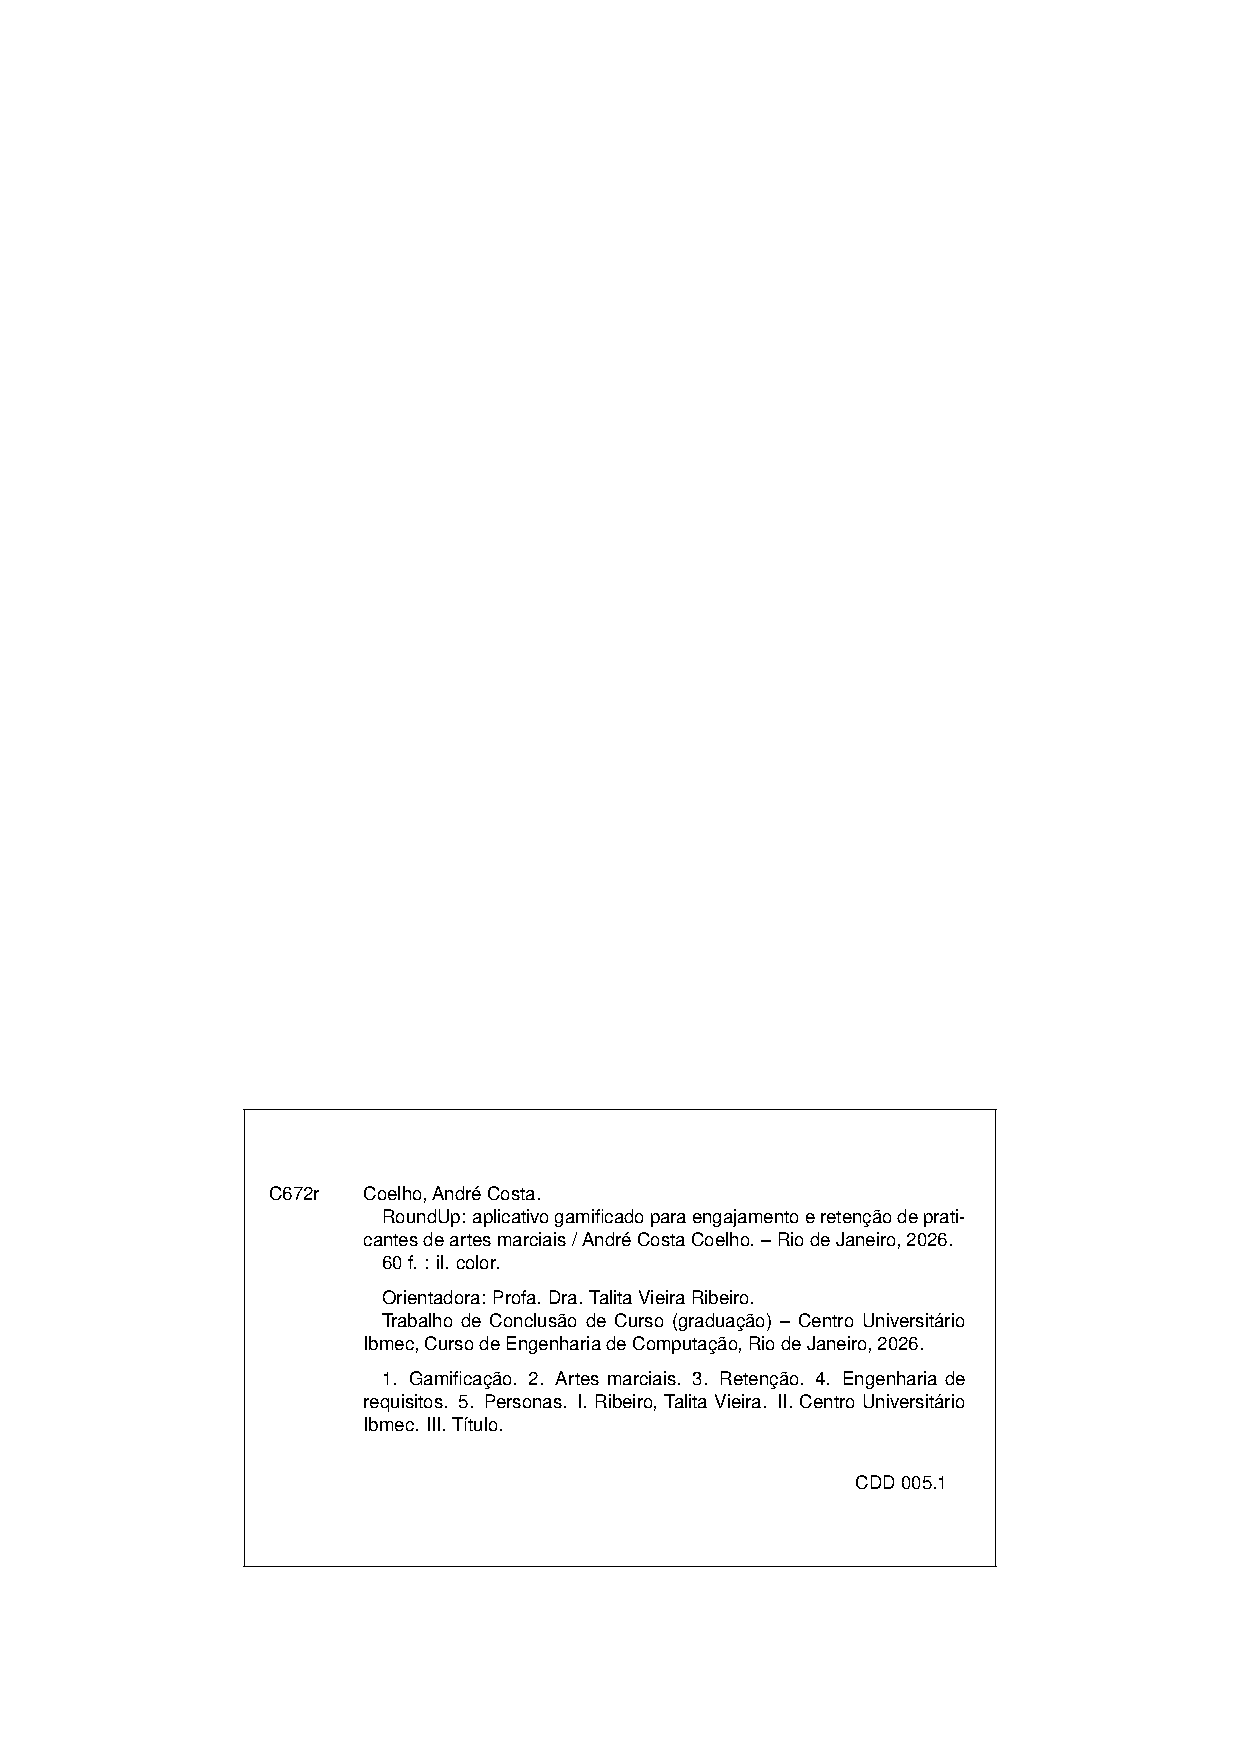
\includepdf[pages=1, pagecommand={\thispagestyle{empty}}]{ficha/ficha-catalografica.pdf}%
}{%
  \begin{fichacatalografica}
    \vspace*{\fill}
    \begin{center}
      \fbox{\begin{minipage}[c][7cm][c]{12.5cm}
        \centering\footnotesize
        \textbf{FICHA CATALOGRÁFICA}\\[8pt]
        Este espaço é o verso da folha de rosto.\\
        Na versão final, gere a ficha catalográfica e salve o PDF\\
        como \texttt{ficha/ficha-catalografica.pdf}.\\
        Ela substituirá este quadro automaticamente.
      \end{minipage}}
    \end{center}
  \end{fichacatalografica}
}

% No modo "oneside" o verso ocupa uma página própria no PDF, mas não é
% uma nova folha -- por isso não deve ser contado (Manual, 3.6).
\makeatletter
\if@twoside\else\addtocounter{page}{-1}\fi
\makeatother
    % obrigatório (+ ficha catalográfica no verso)
% % =====================================================================
%  ERRATA (opcional) -- Manual, seção 2.1.3
%  Só use se, depois de impresso/entregue, você encontrar erros.
%  Para ativar, retire o % da linha % =====================================================================
%  ERRATA (opcional) -- Manual, seção 2.1.3
%  Só use se, depois de impresso/entregue, você encontrar erros.
%  Para ativar, retire o % da linha % =====================================================================
%  ERRATA (opcional) -- Manual, seção 2.1.3
%  Só use se, depois de impresso/entregue, você encontrar erros.
%  Para ativar, retire o % da linha \input{pretextuais/errata} no main.tex.
% =====================================================================
\begin{errata}
  \SingleSpacing
  \noindent\MakeTextUppercase{\imprimirautor}. \textbf{\imprimirtitulo}.
  \imprimirdata. Trabalho de Conclusão de Curso (\imprimirgrau) --
  \imprimirinstituicao, \imprimirlocal, \imprimirdata.

  \vspace{\baselineskip}
  \begin{table}[htb]
    \centering
    \begin{tabular}{cccc}
      \toprule
      \textbf{Folha} & \textbf{Linha} & \textbf{Onde se lê} & \textbf{Leia-se} \\
      \midrule
      10 & 2  & degau   & degrau   \\
      34 & 23 & atólogo & autólogo \\
      \bottomrule
    \end{tabular}
  \end{table}
\end{errata}
 no main.tex.
% =====================================================================
\begin{errata}
  \SingleSpacing
  \noindent\MakeTextUppercase{\imprimirautor}. \textbf{\imprimirtitulo}.
  \imprimirdata. Trabalho de Conclusão de Curso (\imprimirgrau) --
  \imprimirinstituicao, \imprimirlocal, \imprimirdata.

  \vspace{\baselineskip}
  \begin{table}[htb]
    \centering
    \begin{tabular}{cccc}
      \toprule
      \textbf{Folha} & \textbf{Linha} & \textbf{Onde se lê} & \textbf{Leia-se} \\
      \midrule
      10 & 2  & degau   & degrau   \\
      34 & 23 & atólogo & autólogo \\
      \bottomrule
    \end{tabular}
  \end{table}
\end{errata}
 no main.tex.
% =====================================================================
\begin{errata}
  \SingleSpacing
  \noindent\MakeTextUppercase{\imprimirautor}. \textbf{\imprimirtitulo}.
  \imprimirdata. Trabalho de Conclusão de Curso (\imprimirgrau) --
  \imprimirinstituicao, \imprimirlocal, \imprimirdata.

  \vspace{\baselineskip}
  \begin{table}[htb]
    \centering
    \begin{tabular}{cccc}
      \toprule
      \textbf{Folha} & \textbf{Linha} & \textbf{Onde se lê} & \textbf{Leia-se} \\
      \midrule
      10 & 2  & degau   & degrau   \\
      34 & 23 & atólogo & autólogo \\
      \bottomrule
    \end{tabular}
  \end{table}
\end{errata}
          % opcional -- retire o % se precisar
% =====================================================================
%  FOLHA DE APROVAÇÃO (obrigatório) -- Manual, seção 2.1.4
%  Os nomes da banca vêm de config/dados.tex.
%  Leve esta folha impressa no dia da defesa para colher as assinaturas
%  (Regulamento, Art. 15, III). Na versão final, você pode substituir
%  esta página pela folha assinada e digitalizada (veja o LEIA-ME).
% =====================================================================
\IfFileExists{ficha/folha-aprovacao-assinada.pdf}{%
  \includepdf[pages=1, pagecommand={\thispagestyle{empty}}]{ficha/folha-aprovacao-assinada.pdf}%
}{%
\begin{folhadeaprovacao}
  \centering

  {\bfseries\MakeTextUppercase{\imprimirautor}\par}
  \vspace*{1.5cm}

  {\bfseries\OnehalfSpacing\imprimirtitulocompleto\par}
  \vspace*{1.5cm}

  \hspace{.45\textwidth}%
  \begin{minipage}{.55\textwidth}
    \SingleSpacing\raggedright
    \imprimirnatureza
  \end{minipage}
  \vspace*{1cm}

  \begin{flushleft}
    Aprovado em: \dataaprovacao
  \end{flushleft}

  \vspace*{0.5cm}
  {\bfseries BANCA EXAMINADORA\par}

  \membrobanca{\bancaorientador\ (\imprimirrotuloorientador)}{\bancaorientadorinst}
  \membrobanca{\bancaexaminadorum}{\bancaexaminadoruminst}
  \membrobanca{\bancaexaminadordois}{\bancaexaminadordoisinst}

  \vfill
  {\bfseries\MakeTextUppercase{\imprimirlocal}\par\imprimirdata\par}
\end{folhadeaprovacao}
}
% obrigatório
% =====================================================================
%  DEDICATÓRIA (opcional) -- Manual, seção 2.1.5
%  Texto curto, no pé da página, alinhado à direita. Não leva título.
%  Para remover: coloque % na linha % =====================================================================
%  DEDICATÓRIA (opcional) -- Manual, seção 2.1.5
%  Texto curto, no pé da página, alinhado à direita. Não leva título.
%  Para remover: coloque % na linha % =====================================================================
%  DEDICATÓRIA (opcional) -- Manual, seção 2.1.5
%  Texto curto, no pé da página, alinhado à direita. Não leva título.
%  Para remover: coloque % na linha \input{pretextuais/dedicatoria} do main.tex.
% =====================================================================
\begin{dedicatoria}
  \vspace*{\fill}
  \hspace{.5\textwidth}%
  \begin{minipage}{.5\textwidth}
    \raggedright
    À minha família e aos meus amigos,\\
    que caminharam comigo até aqui\\
    e tornaram cada etapa mais leve.
  \end{minipage}
\end{dedicatoria}
 do main.tex.
% =====================================================================
\begin{dedicatoria}
  \vspace*{\fill}
  \hspace{.5\textwidth}%
  \begin{minipage}{.5\textwidth}
    \raggedright
    À minha família e aos meus amigos,\\
    que caminharam comigo até aqui\\
    e tornaram cada etapa mais leve.
  \end{minipage}
\end{dedicatoria}
 do main.tex.
% =====================================================================
\begin{dedicatoria}
  \vspace*{\fill}
  \hspace{.5\textwidth}%
  \begin{minipage}{.5\textwidth}
    \raggedright
    À minha família e aos meus amigos,\\
    que caminharam comigo até aqui\\
    e tornaram cada etapa mais leve.
  \end{minipage}
\end{dedicatoria}
       % opcional -- coloque % na frente para remover
% =====================================================================
%  AGRADECIMENTOS (opcional) -- Manual, seção 2.1.6
%  Linguagem clara, direta e concisa, com os NOMES COMPLETOS das pessoas.
%  Para remover: coloque % na linha correspondente do main.tex.
% =====================================================================
\begin{agradecimentos}
À minha orientadora, Profa. Dra. Talita Vieira Ribeiro, pela orientação,
paciência e pelas contribuições que deram forma a este trabalho.

Aos meus pais, Andréa Costa e Júlio César Coelho, pelo apoio incondicional
ao longo de toda a graduação.

Aos meus avós, Carlos Moraes Costa, Ada Helena Costa, Jomar Coelho e
Jandira Coelho,
pelo carinho e pelo apoio, inclusive financeiro, que tornaram possível a
minha formação.

Aos alunos da academia GFTEAM, que abriram as portas e dedicaram seu tempo
à validação do RoundUp.

Aos professores e colegas do curso de Engenharia de Computação do Centro
Universitário Ibmec, pelos conhecimentos compartilhados durante a graduação.
\end{agradecimentos}
    % opcional
% =====================================================================
%  EPÍGRAFE (opcional) -- Manual, seção 2.1.7
%  Uma citação relacionada ao tema, seguida da indicação de autoria.
%  Fica no pé da página, alinhada à direita. Não leva título.
%  Lembre-se: o autor citado também deve estar nas Referências.
% =====================================================================
\begin{epigrafe}
  \vspace*{\fill}
  \noindent\hspace{.45\textwidth}%
  \begin{minipage}{.55\textwidth}
    \raggedright
    \textit{Nós somos aquilo que fazemos repetidamente. Excelência,
    então, não é um ato, mas um hábito.}

    \begin{flushright}\cite[tradução nossa]{durant1926}\end{flushright}
  \end{minipage}
\end{epigrafe}
          % opcional
% =====================================================================
%  RESUMO EM LÍNGUA PORTUGUESA (obrigatório) -- Manual, seção 2.1.8
% ---------------------------------------------------------------------
%  Regras (ABNT NBR 6028:2021):
%   - UM ÚNICO parágrafo, sem recuo, espaço simples;
%   - entre 150 e 500 palavras;
%   - frases concisas e afirmativas; terceira pessoa do singular e voz
%     ativa ("Este trabalho analisa...", e não "Neste trabalho eu analisei...");
%   - deve apresentar: OBJETIVO, MÉTODO, RESULTADOS e CONCLUSÕES;
%   - sem citações, figuras, tabelas ou equações;
%   - palavras-chave logo abaixo, separadas por ponto e vírgula (;) e
%     terminadas com ponto final (.).
%  DICA: escreva o resumo por último, quando o trabalho estiver pronto.
% =====================================================================
\setlength{\absparsep}{18pt}
\begin{resumo}
\SingleSpacing
\noindent A evasão de praticantes é um problema recorrente em academias de
lutas e artes marciais, e muitos alunos abandonam o treino antes de
perceber os seus benefícios físicos e mentais. Este trabalho apresenta o
RoundUp, um aplicativo móvel gamificado que busca aumentar o engajamento e
a retenção dos alunos e apoiar professores e academias na gestão das
turmas. O projeto foi conduzido como um processo de ideação: treze ideias
de funcionalidades foram convertidas em requisitos, que orientaram a
construção do aplicativo e, ao mesmo tempo, foram avaliados por meio de um
questionário respondido por praticantes e ex-praticantes. Para ampliar a
cobertura dos perfis de usuário, incluindo o de professor, foram
empregadas personas sintéticas e um gerador de respostas desenvolvidos
com apoio de inteligência artificial: a partir de 12 personas, foram
produzidas 65 respostas que permitiram exercitar todo o questionário e o
procedimento de análise, mantidas separadas dos dados reais. O protótipo foi desenvolvido em React
Native com Firebase, com três perfis de usuário (aluno, professor e
academia), e implementa 29 dos 33 requisitos funcionais, entre eles
registro de presença com validação pelo professor, pontos de experiência,
níveis, sequência de treinos, medalhas, classificação, missões, registro
de graduação, relatórios de frequência e consentimento conforme a LGPD. As
regras de negócio que protegem a gamificação foram implementadas nas
regras de segurança do banco de dados e cobertas por testes automatizados.
Na avaliação real, os recursos que tornam o progresso visível, como a
barra de progresso até a graduação e o histórico de presença, tiveram as
melhores notas; lembretes e mensagens automáticas, as piores; e os
comentários apontaram o excesso de notificações e de dados a inserir como
motivos de abandono do aplicativo, o que levou a tornar as notificações
configuráveis e a classificação opcional. Conclui-se que a gamificação
centrada no progresso visível é a direção mais promissora para o
aplicativo, que parte da evasão tem causas externas que um aplicativo não
resolve e que os requisitos de gestão ainda precisam ser avaliados por
professores reais.

\vspace{\onelineskip}
\noindent\textbf{Palavras-chave}: gamificação; artes marciais; retenção; engenharia de requisitos; personas.
\end{resumo}
            % obrigatório
% =====================================================================
%  RESUMO EM LÍNGUA ESTRANGEIRA -- ABSTRACT (obrigatório) -- Manual, 2.1.8.2
%  É a TRADUÇÃO FIEL do resumo em português, incluindo as palavras-chave
%  (Keywords). Mesmas regras de formatação do resumo.
% =====================================================================
\begin{resumo}[Abstract]
\begin{otherlanguage*}{english}
\SingleSpacing
\noindent Dropout is a recurring problem in martial arts and combat sports
gyms, and many students quit before perceiving the physical and mental
benefits of training. This work presents RoundUp, a gamified mobile
application that aims to increase student engagement and retention and to
support instructors and gyms in managing their classes. The project was
conducted as an ideation process: thirteen feature ideas were converted
into requirements, which guided the development of the application and,
at the same time, were evaluated through a questionnaire answered by current
and former practitioners. To broaden the coverage of user profiles,
including the instructor profile, synthetic personas and a response
generator developed with the support of artificial intelligence were
employed: from 12 personas, 65 responses were produced, which made it
possible to exercise the entire questionnaire and the analysis procedure,
and were kept separate from the real data. The prototype was developed with React Native and Firebase, has
three user profiles (student, instructor and gym) and implements 29 of the 33 functional requirements, including attendance check-in validated by
the instructor, experience points, levels, training streaks, badges,
leaderboard, missions, belt promotion records, attendance reports and
consent in compliance with the Brazilian data protection law (LGPD). The
business rules that protect the gamification were implemented in the
database security rules and covered by automated tests. In the real
evaluation, the features that make progress visible, such as the progress
bar toward the next belt and the attendance history, received the highest
scores; reminders and automatic messages, the lowest; and the comments
pointed to excessive notifications and data entry as reasons to abandon
the app, which led to making notifications configurable and the
leaderboard optional. It is concluded that gamification centered on
visible progress is the most promising direction for the application,
that part of the dropout has external causes that an app cannot solve,
and that the next step is to validate the management requirements with
instructors in the field.

\vspace{\onelineskip}
\noindent\textbf{Keywords}: gamification; martial arts; retention; requirements engineering; personas.
\end{otherlanguage*}
\end{resumo}
          % obrigatório
% =====================================================================
%  LISTAS -- Manual, seções 2.1.9 a 2.1.12
% ---------------------------------------------------------------------
%  São OPCIONAIS, mas tornam-se OBRIGATÓRIAS quando houver MAIS DE 5
%  itens do tipo no trabalho. Se tiver 5 ou menos, você pode remover a
%  lista colocando % no início da(s) linha(s) correspondente(s).
%
%  As listas de ilustrações, quadros, tabelas e códigos são geradas
%  AUTOMATICAMENTE a partir dos \caption{} do texto.
%  As listas de siglas e de símbolos são escritas À MÃO, logo abaixo.
% =====================================================================

% --- Lista de ilustrações (figuras, gráficos, fluxogramas, fotos...) ---
\pdfbookmark[0]{\listfigurename}{lof}
\listoffigures*
\cleardoublepage

% --- Lista de quadros (quadro = conteúdo textual, com bordas fechadas) ---
\pdfbookmark[0]{\listofquadrosname}{loq}
\listofquadros*
\cleardoublepage

% --- Lista de tabelas (tabela = dados numéricos, bordas laterais abertas) ---
\pdfbookmark[0]{\listtablename}{lot}
\listoftables*
\cleardoublepage

% --- Lista de códigos (útil no relatório técnico) ---------------------
\ifrelatorio
  \pdfbookmark[0]{\listofcodigosname}{loc}
  \listofcodigos*
  \cleardoublepage
\fi

% --- Lista de abreviaturas e siglas (em ORDEM ALFABÉTICA) -------------
% Na primeira vez que a sigla aparece no texto, escreva o nome completo
% seguido da sigla entre parênteses: "Associação Brasileira de Normas
% Técnicas (ABNT)". Depois, use apenas a sigla.
\begin{siglas}
  \item[ABNT] Associação Brasileira de Normas Técnicas
  \item[CT] Caso de Teste
  \item[IA] Inteligência Artificial
  \item[LGPD] Lei Geral de Proteção de Dados Pessoais
  \item[LLM] \textit{Large Language Model} (modelo de linguagem de grande porte)
  \item[MoSCoW] \textit{Must, Should, Could, Won't} (método de priorização)
  \item[NoSQL] \textit{Not only SQL} (banco de dados não relacional)
  \item[RF] Requisito Funcional
  \item[RN] Regra de Negócio
  \item[RNF] Requisito Não Funcional
  \item[TCC] Trabalho de Conclusão de Curso
  \item[UC] Caso de Uso (\textit{Use Case})
  \item[UML] \textit{Unified Modeling Language}
  \item[WCAG] \textit{Web Content Accessibility Guidelines}
  \item[XP] Pontos de experiência (\textit{experience points})
\end{siglas}

% --- Lista de símbolos (na ORDEM em que aparecem no texto) ------------
% Este trabalho não usa símbolos matemáticos; lista desativada.
% \begin{simbolos}
%   \item[$ \sigma $] Tensão normal
%   \item[$ F $] Força aplicada
%   \item[$ A $] Área da seção transversal
%   \item[$ \in $] Pertence
% \end{simbolos}
            % listas de ilustrações, tabelas, siglas, símbolos
% =====================================================================
%  SUMÁRIO (obrigatório) -- Manual, seção 2.1.13
%  Gerado AUTOMATICAMENTE a partir dos títulos de capítulos e seções.
%  É o último elemento pré-textual. Não precisa editar.
%  Se o sumário aparecer desatualizado, compile o documento mais uma vez.
% =====================================================================
\pdfbookmark[0]{\contentsname}{toc}
\tableofcontents*
\cleardoublepage
           % obrigatório

% ---------------------------------------------------------------------
% ELEMENTOS TEXTUAIS  (a numeração de página começa a aparecer aqui)
% ---------------------------------------------------------------------
\textual

\ifrelatorio
  % ===== PROJETO APLICADO: RELATÓRIO TÉCNICO (Regulamento, Art. 9º) =====
  % =====================================================================
%  CAPÍTULO 1 -- INTRODUÇÃO
%  Formato: PROJETO APLICADO (relatório técnico + protótipo)
%
%  O Manual recomenda texto corrido, sem dividir a introdução em seções.
% =====================================================================

\chapter{Introdução e objetivos}
\label{cap:introducao}

% (a) Contexto e problema
A prática regular de lutas e artes marciais está associada a benefícios
que vão além do condicionamento físico. Em revisão sistemática com
meta-análise, \citeonline{moore2020} encontraram efeitos positivos do
treinamento em artes marciais sobre o bem-estar e a saúde mental dos
praticantes, incluindo a redução de sintomas de ansiedade e depressão.
Esses benefícios, porém, só aparecem com a continuidade do treino. Na
prática das academias, uma parte expressiva dos alunos abandona a
atividade antes de consolidar o hábito, seja pela percepção lenta da
própria evolução, pela falta de metas claras, pelo distanciamento do
professor ou por mudanças na rotina. Para o aluno, o abandono interrompe
o ciclo em que os ganhos se tornariam perceptíveis; para a academia e o
professor, representa perda de receita e de vínculo com a turma.

% (b) Solução proposta
Para enfrentar esse problema, este projeto propõe o \textbf{RoundUp}, um
aplicativo móvel que aplica \textbf{gamificação} -- o uso de elementos de
design de jogos em contextos que não são jogos \cite{deterding2011} -- ao
acompanhamento dos treinos. Para o aluno, o aplicativo oferece mecânicas
como pontos de experiência, sequências de treino, medalhas e uma barra de
progresso rumo à próxima graduação. Para o professor, oferece apoio à
gestão: registro de presença, criação de missões para a turma e alertas
sobre alunos com queda de frequência. O sistema distingue três perfis de
usuário: o \textbf{aluno}, o \textbf{professor}, que pode atuar de forma
autônoma, e a \textbf{academia}, que reúne professores, turmas e alunos.
O protótipo resultante é de natureza \textbf{digital} (Regulamento,
Art.~10): um aplicativo funcional em React Native com \textit{back-end}
no Firebase.

% Natureza de ideação do projeto
Por se tratar de um domínio em que o valor de cada mecânica de jogo para
o público ainda é pouco conhecido, o projeto foi conduzido como um
\textbf{projeto de ideação}. Em vez de partir de requisitos fechados, o
autor elaborou um conjunto de ideias de funcionalidades e as converteu em
\textbf{requisitos iniciais}. Esses mesmos requisitos tiveram dois usos
simultâneos: orientaram a construção do aplicativo e se tornaram os itens
de um questionário de avaliação de ideias (\textit{survey}), respondido
por praticantes e ex-praticantes reais. Como houve poucos respondentes
(seis) e nenhum professor entre eles, foram construídas 12 personas
sintéticas e, a partir delas, geradas 65 \textbf{respostas sintéticas} ao
questionário, com apoio de um modelo de linguagem de grande porte (LLM).
Essas respostas foram usadas para testar o instrumento e o procedimento
de análise, e não como evidência da percepção de usuários. A \autoref{fig:ciclo-ideacao}, no
\autoref{cap:requisitos}, ilustra esse ciclo.

% (c) Objetivos
O objetivo geral deste projeto é \textbf{idear, desenvolver e avaliar o
RoundUp, um aplicativo gamificado para academias de lutas e artes
marciais, voltado a aumentar o engajamento e a retenção dos alunos e a
apoiar o professor na gestão da turma}. Os objetivos específicos são:

\begin{enumerate}
  \item identificar fatores de motivação e de evasão de praticantes de
        lutas e artes marciais;
  \item elaborar ideias de mecânicas de gamificação e de apoio ao
        professor e convertê-las em requisitos iniciais rastreáveis;
  \item avaliar a percepção de valor dessas ideias com usuários reais,
        por meio de um questionário;
  \item construir personas sintéticas e usá-las como insumo
        complementar da ideação e para gerar respostas de teste que
        verifiquem o questionário e o procedimento de análise, sem
        misturá-las aos dados reais;
  \item modelar e implementar um protótipo do aplicativo com os
        requisitos priorizados;
  \item considerar, desde a concepção, a conformidade com a Lei Geral de
        Proteção de Dados Pessoais (LGPD), inclusive no tratamento de dados
        de menores de idade \cite{lgpd2018}.
\end{enumerate}

% (d) Justificativa
O projeto tem relevância social, por contribuir para a permanência de
alunos em uma atividade associada à saúde física e mental; relevância
técnica, por articular engenharia de requisitos, gamificação,
desenvolvimento móvel e proteção de dados pessoais em uma solução
prática; e relevância metodológica, por documentar o uso de personas e
respostas sintéticas como insumo complementar da ideação e como dados de
teste de um instrumento de pesquisa, deixando explícito o que elas podem
e o que não podem mostrar. Soma-se a isso a vivência do autor
com as artes marciais, que facilita o acesso a praticantes e professores.

% (e) Escopo
O escopo do projeto concentra-se em academias de lutas e artes marciais
no Brasil e em duas perspectivas de uso: a do aluno (engajamento) e a do
professor (gestão). Ficam fora do escopo: outras modalidades esportivas,
prescrição de treinos ou orientação nutricional, integração com
dispositivos vestíveis, análise de movimentos por visão computacional e
aspectos comerciais, como monetização e escalabilidade em produção. A
avaliação do impacto de longo prazo sobre a evasão também ultrapassa o
prazo do TCC.

O recorte abrange lutas e artes marciais em geral: o aplicativo não depende de
uma modalidade específica, e o usuário escolhe a sua no cadastro.

% (f) Estrutura do relatório
Este relatório está organizado da seguinte forma: o
\autoref{cap:requisitos} apresenta os fundamentos que orientaram a
ideação, o processo de ideação e os requisitos do projeto; o
\autoref{cap:modelagem}, as modelagens funcional, estática e dinâmica; o
\autoref{cap:implementacao}, as estratégias de implementação do
protótipo; o \autoref{cap:testes}, os procedimentos de avaliação das
ideias com usuários reais, o teste do questionário com respostas
sintéticas e os testes do protótipo; e o \autoref{cap:resultados}, os resultados e as
considerações finais.

  % =====================================================================
%  CAPÍTULO 2 -- IDEAÇÃO E REQUISITOS DO PROJETO
%  (Regulamento, Art. 9º, item ii)
% ---------------------------------------------------------------------
%  Neste projeto, o capítulo de requisitos também descreve o PROCESSO DE
%  IDEAÇÃO, pois os requisitos iniciais nasceram das ideias e foram,
%  depois, avaliados no survey com usuarios reais (ver Capítulo 5).
%
%  Linha do raciocínio (para o aluno não se perder):
%    IDEIA (I01...)  ->  REQUISITO (RF01...)  ->  ITEM DO SURVEY
%                                       ->  NOTA DOS USUÁRIOS REAIS
%                                       ->  DECISÃO (manter, ajustar, adiar)
% =====================================================================

\chapter{Requisitos funcionais e não funcionais}
\label{cap:requisitos}

\section{Fundamentos que orientaram a ideação}
\label{sec:fundamentos}

\subsection{Gamificação}

\citeonline{deterding2011} definem gamificação como o uso de elementos de
design de jogos em contextos que não são jogos. Em saúde e bem-estar, a
revisão sistemática de \citeonline{johnson2016} indica que sistemas
gamificados podem favorecer o engajamento com hábitos saudáveis,
principalmente quando tornam o progresso visível e recompensador, embora
os efeitos variem conforme o desenho da intervenção. Obras de referência
da área \cite{zichermann2011,kapp2012} alertam que as mecânicas devem
servir a objetivos de comportamento bem definidos; caso contrário, viram
apenas uma camada visual sem efeito real.

Para escolher as mecânicas, adotou-se o \textit{framework} Octalysis
\cite{chou2015}, que organiza a motivação humana em oito impulsos
(\textit{core drives}), como o sentido de progresso e realização, a
influência social e o medo de perder algo conquistado. Complementarmente,
a Teoria da Autodeterminação \cite{ryan2000} lembra que a motivação mais
duradoura depende da sensação de competência, de autonomia e de
pertencimento -- e que recompensas externas mal aplicadas podem enfraquecer
a motivação interna. Essa ressalva é especialmente relevante para
mecânicas competitivas, como \textit{rankings}.

\subsection{Personas}

Uma \textbf{persona} é um personagem fictício, porém fundamentado em
dados, que representa um grupo de usuários com objetivos e
comportamentos semelhantes \cite{cooper1999,pruitt2006}. Neste projeto,
além de orientar o design, as personas serviram de base para gerar
\textbf{respostas sintéticas} ao questionário, usadas como dados de teste
do instrumento e da análise. Estudos recentes mostram que modelos de
linguagem conseguem reproduzir, em alguma medida, padrões de resposta de
grupos humanos \cite{argyle2023,aher2023}, mas também apontam distorções,
como respostas mais homogêneas e estereotipadas do que as de pessoas
reais. Por isso, as personas e as respostas derivadas delas foram
tratadas como \textbf{insumo complementar da ideação}, nunca como
substitutas da opinião de usuários reais: ao representar perfis ausentes
da amostra, como o professor e o dono de academia, elas levaram o autor
a revisitar os requisitos, mas a decisão sobre cada um se apoiou nos
dados reais e na literatura.

\section{Processo de ideação}
\label{sec:processo-ideacao}

O projeto seguiu um modelo iterativo e incremental combinado com
prototipação \cite{sommerville2019,pressman2021}, adequado quando parte
dos requisitos é desconhecida no início -- aqui, sobretudo, o valor que
cada mecânica de jogo tem para alunos e professores. A
\autoref{fig:ciclo-ideacao} resume o ciclo seguido.

\begin{figure}[!htb]
  \centering
  \caption{Ciclo de ideação adotado no projeto}
  \label{fig:ciclo-ideacao}
  \begin{tikzpicture}[
      font=\footnotesize,
      etapa/.style={draw, rounded corners=3pt, align=center,
                    minimum width=3.0cm, minimum height=1.0cm, fill=white},
      seta/.style={-{Stealth[length=2.5mm]}, thick},
      node distance=0.6cm and 0.9cm]
    \node[etapa] (ideias) {1. Ideias de\\funcionalidades};
    \node[etapa, right=of ideias] (req) {2. Requisitos\\iniciais (RF/RNF)};
    \node[etapa, above right=0.3cm and 0.9cm of req] (app) {3a. Construção\\do aplicativo};
    \node[etapa, right=of req] (survey) {3b. \textit{Survey} com\\usuários reais};
    \node[etapa, below right=0.3cm and 0.9cm of req] (pers) {3c. Personas e\\respostas sintéticas};
    \node[etapa, right=4.6cm of req] (cons) {4. Consolidação\\e priorização};
    \draw[seta] (ideias) -- (req);
    \draw[seta] (req) -- (app);
    \draw[seta] (req) -- (survey);
    \draw[seta] (req) -- (pers);
    \draw[seta] (survey) -- (cons);
    \draw[seta, dashed] (pers.east) -| node[pos=0.8, right, font=\scriptsize, align=left]{insumo\\complementar} (cons.south);
    \draw[seta, dashed] (cons.north) -- ++(0,1.55) -| node[pos=0.25, above]{requisitos revisados} (app.north);
  \end{tikzpicture}
  \fonte{Elaborado pelo autor (2026).}
\end{figure}

As etapas foram as seguintes:

\begin{enumerate}
  \item \textbf{Geração de ideias.} A partir da vivência do autor como
        praticante, da literatura
        (\autoref{sec:fundamentos}) e da observação de aplicativos que
        mantêm hábitos com pontos, metas e sequências (como o Duolingo) e
        de plataformas brasileiras de gestão de academias de luta, foram
        listadas ideias de funcionalidades para o aluno e para o
        professor.
  \item \textbf{Conversão em requisitos iniciais.} Cada ideia recebeu um
        código (I01, I02\ldots) e deu origem a um ou mais requisitos
        funcionais verificáveis (\autoref{sec:rf}). Os requisitos foram
        registrados em uma base no Notion, com descrição, ator, ciclo de
        desenvolvimento, origem, prioridade (MoSCoW) e situação.
  \item \textbf{Uso duplo dos requisitos.} Os requisitos iniciais
        guiaram a construção do aplicativo (\autoref{cap:implementacao}) e,
        em paralelo, viraram itens do questionário de avaliação, em que o
        respondente atribui uma nota de 1 (pouco útil) a 5 (muito útil) a
        cada recurso.
  \item \textbf{Avaliação por usuários reais e teste com respostas
        sintéticas.} O questionário foi respondido por praticantes e
        ex-praticantes em 18 e 19 de setembro de 2026. Em 26 de outubro
        de 2026, 65 respostas sintéticas, geradas a partir de personas,
        foram registradas em uma cópia separada do formulário para testar
        o instrumento e a análise (\autoref{cap:testes}). As personas e
        essas respostas entraram na consolidação como insumo
        complementar, para repensar os requisitos; as notas que definiram
        a situação de cada um vieram só das respostas reais.
  \item \textbf{Consolidação.} As notas e os comentários foram usados
        para revisar a situação de cada requisito ligado a uma ideia e
        para reforçar requisitos não funcionais de privacidade, de
        controle de notificações e de baixo esforço de registro.
\end{enumerate}

Durante a ideação, uma decisão de modelagem alterou o conjunto de
requisitos: além do aluno e do professor, a \textbf{academia} passou a ser
um perfil próprio, que gerencia professores e turmas, enquanto o professor
pode atuar vinculado a uma academia ou de forma autônoma. Essa decisão
originou os requisitos de vínculo (RF07 a RF09) e as regras RN05 a RN07,
que não correspondem a nenhuma ideia do questionário, mas são condição
para que as ideias funcionem nos dois arranjos encontrados na prática.

\section{Ideias iniciais}
\label{sec:ideias}

O \autoref{qua:ideias} apresenta as ideias iniciais, o perfil a que se
destinam, o impulso motivacional do Octalysis \cite{chou2015} a que cada
uma se relaciona e os requisitos funcionais que ela originou
(\autoref{sec:rf}).

\begin{quadro}[!htb]
  \caption{Ideias iniciais de funcionalidades}
  \label{qua:ideias}
  \centering
  \footnotesize
  \begin{tabular}{|c|p{4.6cm}|c|p{3.9cm}|p{2.0cm}|}
    \hline
    \textbf{ID} & \textbf{Ideia} & \textbf{Perfil} & \textbf{Impulso (Octalysis)} & \textbf{Requisitos} \\ \hline
    I01 & Pontos de experiência (XP) a cada treino & Aluno & Desenvolvimento e realização & RF16 \\ \hline
    I02 & Registro rápido de presença (\textit{check-in}) & Ambos & -- (base do sistema) & RF13, RF22 \\ \hline
    I03 & Contador de dias treinados e frequência semanal & Ambos & Desenvolvimento e realização & RF15, RF24 \\ \hline
    I04 & Ofensiva: sequência de treinos sem falhar & Aluno & Perda e evitação & RF21 \\ \hline
    I05 & Missões e desafios semanais criados pelo professor & Ambos & Empoderamento da criatividade e \textit{feedback} & RF18, RF23 \\ \hline
    I06 & \textit{Ranking} de frequência da turma & Aluno & Influência social e pertencimento & RF20 \\ \hline
    I07 & Medalhas por marcos (100 treinos, 1 ano) & Aluno & Desenvolvimento e realização & RF19 \\ \hline
    I08 & Barra de progresso até a próxima graduação & Aluno & Desenvolvimento e realização & RF17, RF25 \\ \hline
    I09 & Histórico de presença e evolução pessoal & Aluno & Propriedade e posse & RF15 \\ \hline
    I10 & Mural (\textit{feed}) com conquistas da turma & Aluno & Influência social e pertencimento & -- \\ \hline
    I11 & Lembretes nos dias habituais de treino & Aluno & -- (gatilho externo) & RF31 \\ \hline
    I12 & Alerta ao professor e mensagem após ausência & Ambos & Influência social e pertencimento & RF32 \\ \hline
    I13 & Relatório de frequência e evolução da turma & Professor & -- (gestão) & RF26, RF27 \\ \hline
  \end{tabular}
  \fonte{Elaborado pelo autor (2026).}
\end{quadro}

A ideia I10 (mural da turma) foi a única que não originou requisito: ela
ficou fora do escopo definido para esta versão e, na avaliação
(\autoref{cap:testes}), recebeu nota média de 2,5 entre os
ex-praticantes reais, o que reforçou a decisão de não incorporá-la nesta
versão.

\section{Requisitos funcionais}
\label{sec:rf}

Os requisitos funcionais foram escritos no formato ``O sistema deve\ldots'',
priorizados pelo método MoSCoW (\textit{Must}, \textit{Should},
\textit{Could}, \textit{Won't}) e distribuídos em quatro ciclos de
desenvolvimento: Ciclo~1, contas, vínculos e treinos; Ciclo~2,
gamificação; Ciclo~3, gestão; e Ciclo~4, conformidade e retenção. Para
caber na página, as descrições abaixo estão resumidas; o texto integral de
cada requisito está na base de requisitos do projeto.

Nos quadros a seguir, a coluna ``Ideia'' liga o requisito à ideia que o
originou (``--'' indica requisito de base, sem ideia correspondente no
questionário), e a coluna ``Situação'' registra a decisão tomada após a
avaliação descrita no \autoref{cap:testes}, com a seguinte legenda:
\textit{Mantido}, nota média igual ou superior a 3,5 entre os usuários
reais, sem objeções nos comentários; \textit{Ajustado}, mantido, mas com
mudança motivada pelas notas, pelos comentários ou pela literatura;
\textit{A revisar}, nota média abaixo de 3,5 ou avaliação dividida entre
praticantes e ex-praticantes; \textit{Sem dados}, recurso voltado ao
professor, sem respondentes reais desse perfil; \textit{Base}, requisito
estrutural que não foi submetido à avaliação. As personas e as respostas
sintéticas (\autoref{sec:val-personas}) ajudaram a repensar os
requisitos, mas não entraram no cálculo das notas que definem essa
situação.

\begin{quadro}[!htb]
  \caption{Requisitos funcionais dos Ciclos 1 e 2}
  \label{qua:rf}
  \centering
  \footnotesize
  \begin{tabular}{|c|p{7.3cm}|c|c|c|p{1.6cm}|}
    \hline
    \textbf{ID} & \textbf{Descrição resumida} & \textbf{Ideia} & \textbf{Ciclo} & \textbf{Prior.} & \textbf{Situação} \\ \hline
    RF01 & O sistema deve permitir o cadastro escolhendo o perfil Aluno, Professor ou Academia. & -- & 1 & M & Base \\ \hline
    RF02 & O sistema deve permitir login, encerramento de sessão e recuperação de senha. & -- & 1 & M & Base \\ \hline
    RF03 & O sistema deve liberar a cada perfil apenas as funcionalidades correspondentes. & -- & 1 & M & Base \\ \hline
    RF04 & O sistema deve permitir que a academia mantenha seu perfil institucional. & -- & 1 & M & Base \\ \hline
    RF05 & O sistema deve permitir que o professor mantenha seu perfil e indique se é autônomo. & -- & 1 & M & Base \\ \hline
    RF06 & O sistema deve permitir que o aluno edite seu perfil (nome, modalidade, faixa, foto). & -- & 1 & M & Base \\ \hline
    RF07 & O sistema deve permitir vincular professor a academia, com solicitação e aceite. & -- & 1 & M & Base \\ \hline
    RF08 & O sistema deve permitir vincular o aluno a uma academia ou a um professor autônomo. & -- & 1 & M & Base \\ \hline
    RF10 & O sistema deve permitir criar e manter turmas (nome, modalidade, nível, responsável). & -- & 1 & M & Base \\ \hline
    RF11 & O sistema deve permitir matricular o aluno em turmas do seu vínculo ativo. & -- & 1 & M & Base \\ \hline
    RF12 & O sistema deve permitir criar sessões de treino, inclusive a partir de grade semanal. & -- & 1 & M & Base \\ \hline
    RF13 & O sistema deve permitir que o aluno faça \textit{check-in} em uma sessão da sua turma. & I02 & 1 & M & Ajustado \\ \hline
    RF14 & O sistema deve exibir ao aluno a agenda das próximas sessões. & -- & 1 & M & Base \\ \hline
    RF15 & O sistema deve exibir ao aluno o histórico de \textit{check-ins} validados. & I03, I09 & 1 & M & Mantido \\ \hline
    RF16 & O sistema deve creditar XP por \textit{check-ins} validados e missões concluídas. & I01 & 2 & M & Mantido \\ \hline
    RF17 & O sistema deve exibir o nível atual, o XP acumulado e o quanto falta para o próximo nível. & I08 & 2 & M & Ajustado \\ \hline
    RF18 & O sistema deve exibir ao aluno as missões ativas e o progresso em cada uma. & I05 & 2 & M & A revisar \\ \hline
    RF19 & O sistema deve conceder medalhas ao atingir marcos predefinidos. & I07 & 2 & M & Mantido \\ \hline
    RF20 & O sistema deve exibir a classificação por pontos, no escopo do vínculo do aluno. & I06 & 2 & M & Ajustado \\ \hline
    RF21 & O sistema deve contabilizar e exibir a sequência de treinos consecutivos. & I04 & 2 & S & Mantido \\ \hline
  \end{tabular}
  \fonte{Elaborado pelo autor (2026). Prior.: M = \textit{Must}; S = \textit{Should}.}
\end{quadro}

\begin{quadro}[!htb]
  \caption{Requisitos funcionais dos Ciclos 3 e 4}
  \label{qua:rf2}
  \centering
  \footnotesize
  \begin{tabular}{|c|p{7.3cm}|c|c|c|p{1.6cm}|}
    \hline
    \textbf{ID} & \textbf{Descrição resumida} & \textbf{Ideia} & \textbf{Ciclo} & \textbf{Prior.} & \textbf{Situação} \\ \hline
    RF09 & O sistema deve permitir que a academia aceite e encerre vínculos com professores. & -- & 3 & S & Base \\ \hline
    RF22 & O sistema deve permitir que o responsável valide ou rejeite os \textit{check-ins}. & I02 & 3 & M & Sem dados \\ \hline
    RF23 & O sistema deve permitir criar missões personalizadas (critério, recompensa, vigência). & I05 & 3 & M & A revisar \\ \hline
    RF24 & O sistema deve exibir os alunos sob responsabilidade do gestor e sua frequência recente. & I03 & 3 & M & Sem dados \\ \hline
    RF25 & O sistema deve permitir registrar a graduação de faixa ou grau do aluno. & I08 & 3 & M & Ajustado \\ \hline
    RF26 & O sistema deve apresentar relatório de frequência por turma e por período. & I13 & 3 & S & Sem dados \\ \hline
    RF27 & O sistema deve apresentar à academia uma visão consolidada com indicadores agregados. & I13 & 3 & S & Sem dados \\ \hline
    RF33 & O sistema deve permitir ao gestor personalizar pontuação, níveis e faixas. & -- & 3 & S & Base \\ \hline
    RF28 & O sistema deve registrar o consentimento LGPD no cadastro. & -- & 4 & M & Base \\ \hline
    RF29 & O sistema deve permitir que o usuário solicite a exclusão da conta e dos dados. & -- & 4 & M & Base \\ \hline
    RF30 & O sistema deve registrar o responsável legal de alunos menores de 18 anos. & -- & 4 & M & Base \\ \hline
    RF31 & O sistema deve enviar notificações de sessão, nova missão e conquista. & I11 & 4 & S & Ajustado \\ \hline
    RF32 & O sistema deve sinalizar ao gestor os alunos com queda relevante de frequência. & I12 & 4 & S & Ajustado \\ \hline
  \end{tabular}
  \fonte{Elaborado pelo autor (2026). Prior.: M = \textit{Must}; S = \textit{Should}.}
\end{quadro}

Os ajustes indicados nos quadros foram os seguintes. Em RF13, o
\textit{check-in} teve média de 3,2, e um respondente citou ``inserir muitos
dados constantemente'' como motivo para desinstalar o aplicativo; por ser a
base do sistema, ele foi mantido, mas com a exigência de baixo esforço
(RNF01). Em RF17 e RF25, a ``barra de progresso até a próxima graduação''
(I08) passou a ser exibida como progresso de nível por XP, porque a troca
de faixa é sempre uma decisão do professor (RN03), e não um limiar
automático. Em RF20, o \textit{ranking} teve média de 3,7, mas a
disposição a usar o aplicativo com dados visíveis só para o aluno e o
professor variou de 1 a 4, e a literatura alerta para o efeito de
recompensas competitivas sobre a motivação interna; por isso, a
classificação ganhou a exigência de adesão opcional (RNF11) e de janela de
tempo (RN04). Em RF31, os lembretes tiveram a menor média entre as ideias
apresentadas a todos (3,0), e as notificações em excesso foram citadas
como motivo de abandono; as notificações passaram a ser configuráveis por
tipo. Em RF32, a mensagem automática após ausência foi a ideia pior
avaliada pelos ex-praticantes (2,5); manteve-se apenas o alerta ao
professor, cuja utilidade ainda precisa ser avaliada por professores
reais. As missões (RF18 e RF23) ficaram ``a revisar'' porque tiveram média
de 3,2 e foram mal avaliadas pelos ex-praticantes (2,5). Os requisitos
voltados à gestão (RF22, RF24, RF26 e RF27) ficaram ``sem dados'', pois
nenhum professor real respondeu ao questionário.

\section{Regras de negócio}
\label{sec:rn}

As regras de negócio (\autoref{qua:rn}) restringem o comportamento dos
requisitos funcionais. Várias delas protegem a credibilidade da
gamificação, impedindo que o aluno acumule pontos sem ter treinado.

\begin{quadro}[!htb]
  \caption{Regras de negócio}
  \label{qua:rn}
  \centering
  \footnotesize
  \begin{tabular}{|c|p{11.6cm}|c|}
    \hline
    \textbf{ID} & \textbf{Regra} & \textbf{Ciclo} \\ \hline
    RN01 & Pontos só são creditados após o \textit{check-in} ser validado pelo responsável da sessão. & 2 \\ \hline
    RN02 & É permitido no máximo um \textit{check-in} por aluno por sessão de treino. & 1 \\ \hline
    RN03 & A graduação de faixa é sempre decisão do professor ou da academia, nunca automática por pontos. & 3 \\ \hline
    RN04 & A classificação considera apenas os pontos do período vigente. & 2 \\ \hline
    RN05 & Todo aluno precisa de ao menos um vínculo ativo, com academia ou professor autônomo. & 1 \\ \hline
    RN06 & O vínculo entre professor e academia é opcional e depende do aceite das duas partes. & 1 \\ \hline
    RN07 & Toda turma tem um único responsável, e toda sessão pertence a uma turma. & 1 \\ \hline
    RN08 & O \textit{check-in} só é permitido dentro da janela de tempo da sessão. & 1 \\ \hline
    RN09 & A classificação segue o escopo do vínculo: academia, turma ou alunos do professor autônomo. & 2 \\ \hline
  \end{tabular}
  \fonte{Elaborado pelo autor (2026).}
\end{quadro}

\section{Requisitos não funcionais}
\label{sec:rnf}

O \autoref{qua:rnf} apresenta os requisitos não funcionais, classificados
segundo as características de qualidade da ISO/IEC 25010 e os requisitos
organizacionais e legais do projeto. Os comentários dos respondentes do
questionário reforçaram três deles: RNF01 (esforço de registro), RNF11
(adesão opcional à classificação) e, indiretamente, o controle de
notificações previsto em RF31.

\begin{quadro}[!htb]
  \caption{Requisitos não funcionais}
  \label{qua:rnf}
  \centering
  \footnotesize
  \begin{tabular}{|c|p{2.3cm}|p{7.0cm}|p{3.6cm}|}
    \hline
    \textbf{ID} & \textbf{Categoria} & \textbf{Descrição} & \textbf{Critério de aceitação} \\ \hline
    RNF01 & Usabilidade & O \textit{check-in} deve exigir pouco esforço. & Até 3 toques a partir da tela inicial. \\ \hline
    RNF02 & Desempenho & As telas principais devem carregar rapidamente em rede móvel. & Até 3 s em conexão 4G. \\ \hline
    RNF03 & Segurança & Senhas armazenadas de forma criptografada, com gestão delegada ao Firebase Authentication. & Nenhuma senha gravada no banco do app. \\ \hline
    RNF04 & Segurança & Dados de uma academia ou professor não acessíveis por outro; aluno não acessa dados de outro aluno, exceto a classificação. & Regras de segurança do banco cobertas por testes. \\ \hline
    RNF05 & Compatibilidade & Funcionar em Android e iOS. & Android 8.0+ e iOS 14+. \\ \hline
    RNF06 & Confiabilidade & Preservar ações feitas sem conexão e sincronizá-las depois. & Ação concluída após reconexão. \\ \hline
    RNF07 & Organizacional & Desenvolvimento em React Native com Expo e Firebase. & Pilha adotada no repositório. \\ \hline
    RNF08 & Organizacional & Código versionado em Git com repositório remoto. & Histórico de \textit{commits} por ciclo. \\ \hline
    RNF09 & Organizacional & Modelagem UML e protótipo no Figma antes da codificação. & Diagramas e protótipo produzidos. \\ \hline
    RNF10 & Legal & Tratamento de dados conforme a LGPD, com coleta limitada à finalidade \cite{lgpd2018}. & Consentimento registrado; minimização de dados. \\ \hline
    RNF11 & Ético & Participação na classificação opcional para o aluno. & Aluno pode sair do \textit{ranking}. \\ \hline
  \end{tabular}
  \fonte{Elaborado pelo autor (2026).}
\end{quadro}


  % =====================================================================
%  CAPÍTULO 3 -- MODELAGEM DA SOLUÇÃO
%  (Regulamento, Art. 9º, item iii)
% ---------------------------------------------------------------------
%  Três "olhares" complementares:
%   - FUNCIONAL: O QUE o sistema faz para cada usuário (casos de uso);
%   - ESTÁTICO:  DE QUE o sistema é feito (modelo de dados);
%   - DINÂMICO:  COMO o sistema se comporta ao longo do tempo.
%  Os diagramas deste capítulo são desenhados em TikZ, direto no LaTeX.
% =====================================================================

\chapter{Modelagem funcional, estática e dinâmica}
\label{cap:modelagem}

O RoundUp é composto por um aplicativo móvel, usado pelos três perfis, e
por serviços gerenciados do Firebase: autenticação (Firebase
Authentication), banco de dados de documentos (Cloud Firestore),
armazenamento de arquivos (Cloud Storage) e funções executadas no servidor
(Cloud Functions). As regras de acesso aos dados ficam nas regras de
segurança do Firestore, e as regras de gamificação (pontos, níveis,
sequência e medalhas) são aplicadas a partir dos registros de presença
validados.

\section{Modelagem funcional}
\label{sec:modelagem-funcional}

O sistema possui três atores. O \textbf{aluno} registra presença e
acompanha a própria evolução. O \textbf{professor} gerencia turmas,
sessões, presenças, missões e graduações. A \textbf{academia} pode fazer
tudo o que o professor faz e, além disso, gerencia os professores
vinculados a ela e consulta uma visão consolidada. Por isso, nos
diagramas de casos de uso, a academia aparece como especialização do
professor: ela herda os casos de uso de gestão e acrescenta os seus. Essa
generalização foi uma correção feita durante o projeto, que antes tratava
apenas dois atores, e se refletiu em todos os artefatos seguintes:
requisitos, modelo de dados, regras de segurança e protótipo de telas,
cujas visões de professor e academia compartilham a mesma estrutura de
``gestor''.

Os requisitos funcionais originaram 30 casos de uso (UC01 a UC30),
organizados nas mesmas sete categorias da base de requisitos. A
\autoref{fig:casos-uso} mostra a visão geral, com os pacotes e os atores
que participam de cada um, e as figuras seguintes detalham os casos de
uso de cada pacote. Os diagramas foram modelados em PlantUML, e o código
de cada um acompanha o projeto.

\begin{figure}[!htb]
  \centering
  \caption{Visão geral dos casos de uso do RoundUp, por pacote}
  \label{fig:casos-uso}
  \begin{tikzpicture}[
      font=\scriptsize,
      pac/.style={draw, minimum width=3.6cm, minimum height=0.75cm, align=center, fill=black!5},
      ator/.style={align=center},
      lig/.style={thin},
      ger/.style={-{Triangle[open,length=2.5mm,width=2.5mm]}, thin}]
    \node[draw, rounded corners=2pt, minimum width=5.2cm, minimum height=8.6cm] (sis) at (0,0) {};
    \node[anchor=north west] at (sis.north west) {\textbf{RoundUp}};
    \node[pac] (con) at (0, 3.1) {Contas (UC01--UC05)};
    \node[pac] (vin) at (0, 2.0) {Vínculos (UC06--UC08)};
    \node[pac] (ges) at (0, 0.9) {Gestão (UC20--UC25)};
    \node[pac] (tre) at (0,-0.2) {Treinos (UC09--UC15)};
    \node[pac] (cnf) at (0,-1.3) {Conformidade (UC26--UC28)};
    \node[pac] (ret) at (0,-2.4) {Retenção (UC29--UC30)};
    \node[pac] (gam) at (0,-3.5) {Gamificação (UC16--UC19)};
    \node[ator] (al) at (-5.2,-0.3) {\Large$\bigcirc$\\[-1pt]\textbf{Aluno}};
    \node[ator] (pr) at (5.2,-0.9) {\Large$\bigcirc$\\[-1pt]\textbf{Professor}};
    \node[ator] (ac) at (5.2, 2.7) {\Large$\bigcirc$\\[-1pt]\textbf{Academia}};
    \foreach \p in {con,vin,tre,cnf,ret,gam} \draw[lig] (al.east) -- (\p.west);
    \foreach \p in {con,vin,ges,tre,cnf,ret} \draw[lig] (pr.west) -- (\p.east);
    \foreach \p in {con,vin,ges} \draw[lig] (ac.west) -- (\p.east);
    \draw[ger] (ac.south) -- (pr.north);
  \end{tikzpicture}
  \fonte{Elaborado pelo autor (2026). A academia herda os pacotes do
         professor; as linhas da academia indicam os pacotes com casos de
         uso exclusivos dela.}
\end{figure}

\begin{figure}[!htb]
  \centering
  \caption{Casos de uso do pacote Contas}
  \label{fig:uc-contas}
  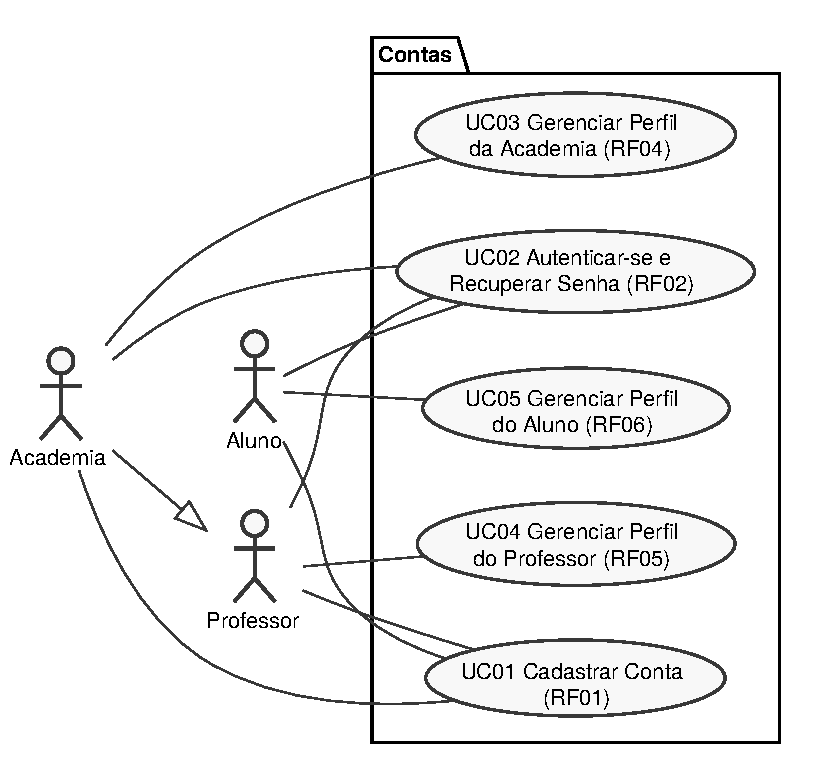
\includegraphics[width=0.62\textwidth]{figuras/uc-1-contas.pdf}
  \fonte{Elaborado pelo autor (2026).}
\end{figure}

\begin{figure}[!htb]
  \centering
  \caption{Casos de uso do pacote Vínculos}
  \label{fig:uc-vinculos}
  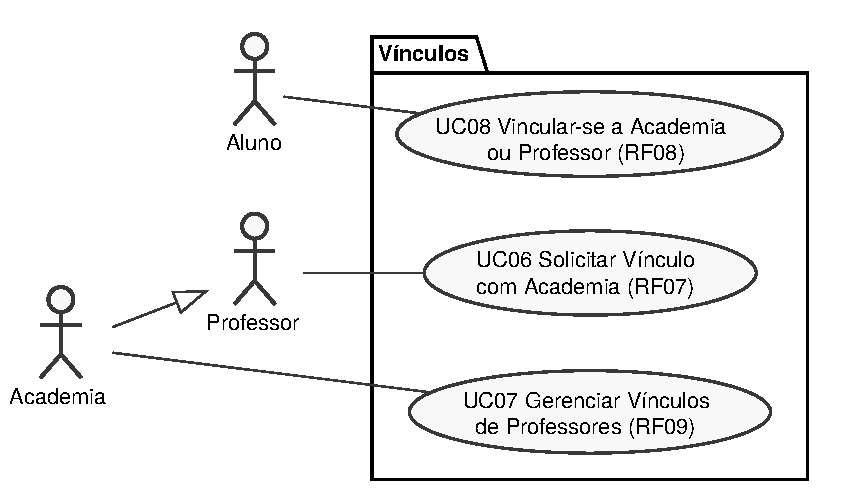
\includegraphics[width=0.62\textwidth]{figuras/uc-2-vinculos.pdf}
  \fonte{Elaborado pelo autor (2026).}
\end{figure}

\begin{figure}[!htb]
  \centering
  \caption{Casos de uso do pacote Treinos}
  \label{fig:uc-treinos}
  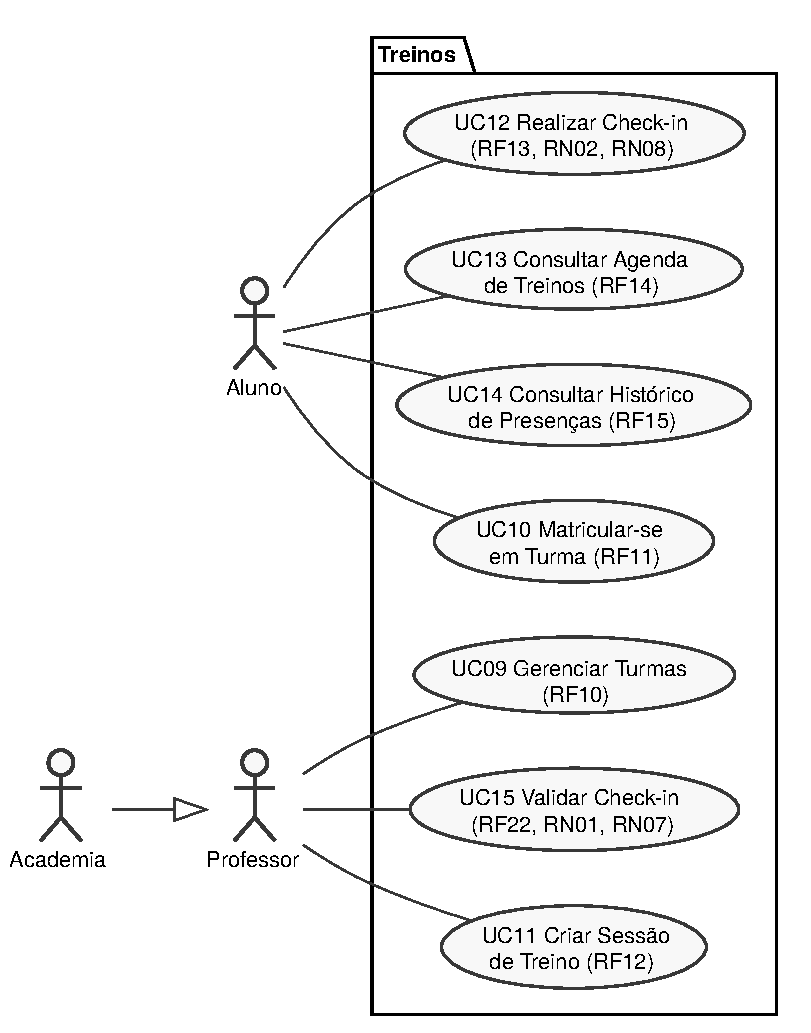
\includegraphics[width=0.62\textwidth]{figuras/uc-3-treinos.pdf}
  \fonte{Elaborado pelo autor (2026).}
\end{figure}

\begin{figure}[!htb]
  \centering
  \caption{Casos de uso do pacote Gamificação}
  \label{fig:uc-gamificacao}
  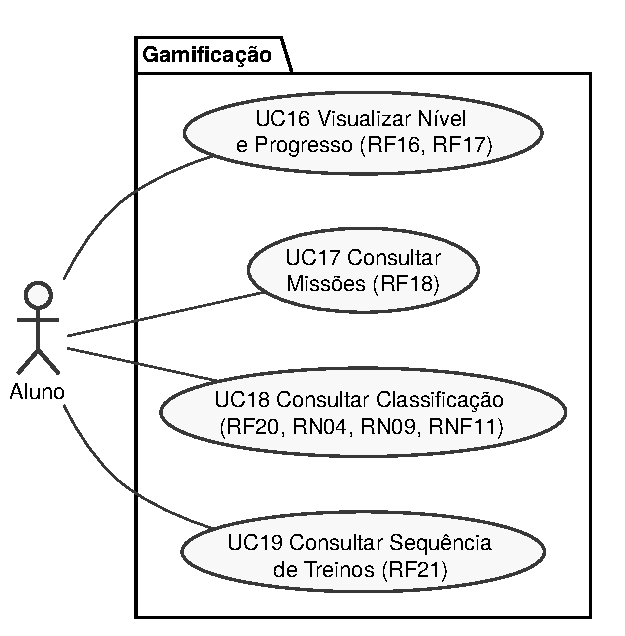
\includegraphics[width=0.5\textwidth]{figuras/uc-4-gamificacao.pdf}
  \fonte{Elaborado pelo autor (2026).}
\end{figure}

\begin{figure}[!htb]
  \centering
  \caption{Casos de uso do pacote Gestão}
  \label{fig:uc-gestao}
  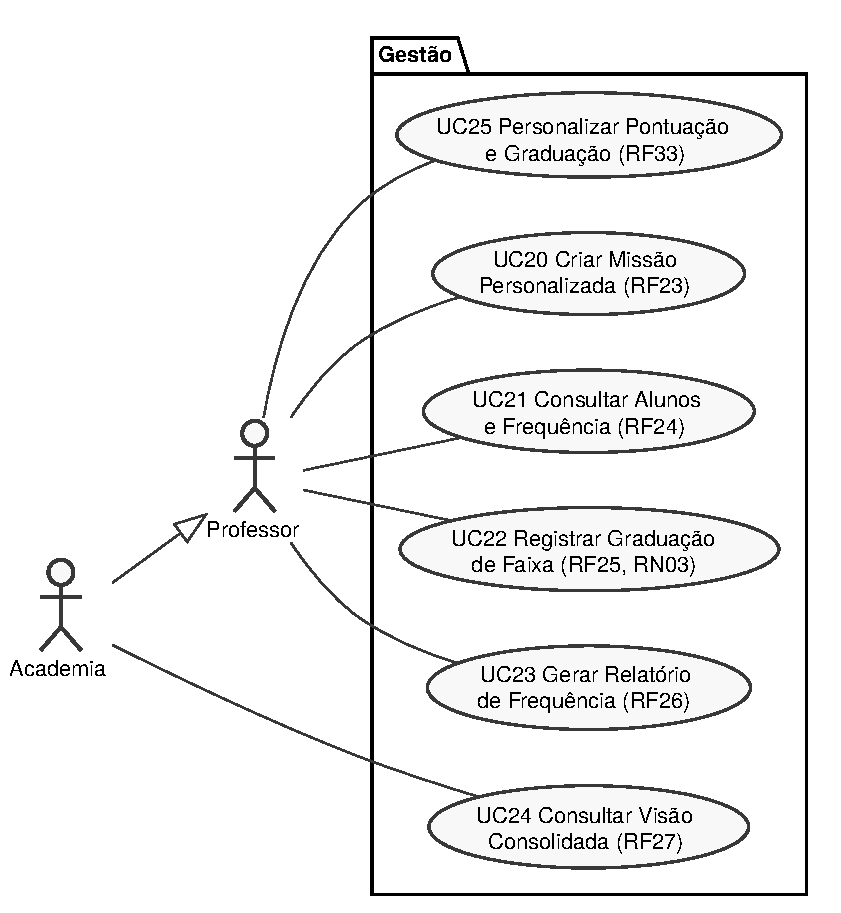
\includegraphics[width=0.62\textwidth]{figuras/uc-5-gestao.pdf}
  \fonte{Elaborado pelo autor (2026).}
\end{figure}

\begin{figure}[!htb]
  \centering
  \caption{Casos de uso do pacote Conformidade}
  \label{fig:uc-conformidade}
  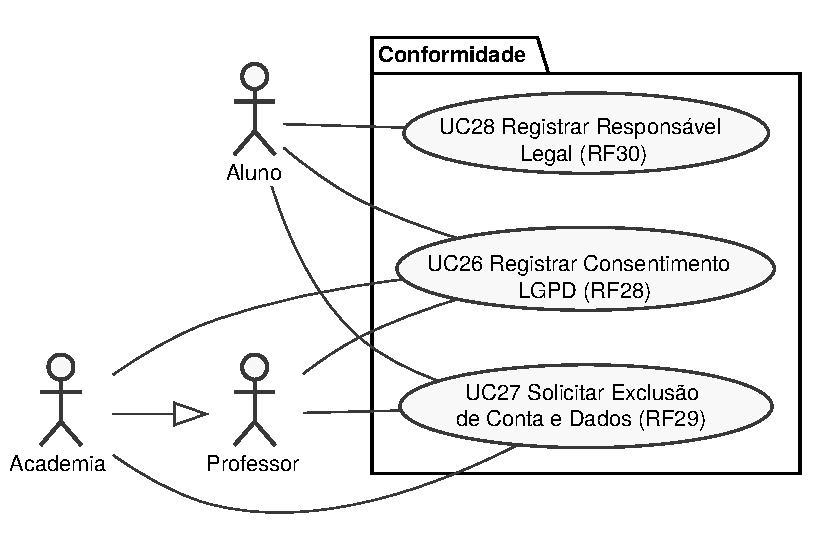
\includegraphics[width=0.62\textwidth]{figuras/uc-6-conformidade.pdf}
  \fonte{Elaborado pelo autor (2026).}
\end{figure}

\begin{figure}[!htb]
  \centering
  \caption{Casos de uso do pacote Retenção}
  \label{fig:uc-retencao}
  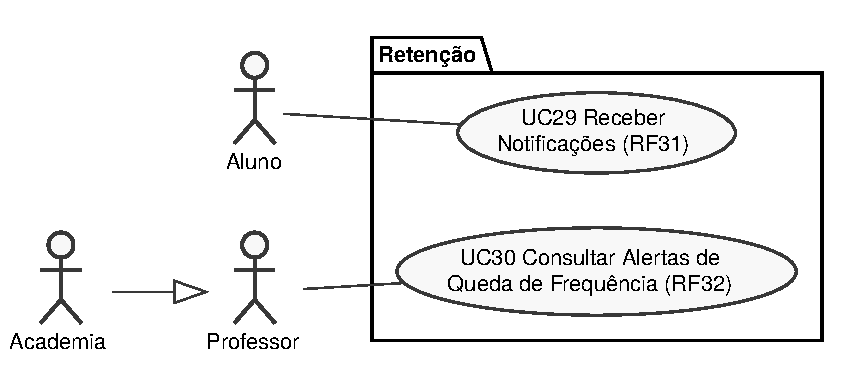
\includegraphics[width=0.62\textwidth]{figuras/uc-7-retencao.pdf}
  \fonte{Elaborado pelo autor (2026).}
\end{figure}

Cada caso de uso traz, no próprio diagrama, os requisitos que atende. A
especificação textual completa de cada um, com atores, pré-condições,
fluxos e pós-condições, está no repositório do projeto (\autoref{ap:artefatos}). A situação de
implementação de cada requisito está na
\autoref{sec:situacao-implementacao}.

\subsection{Descrição dos casos de uso principais}

O caso de uso central do aplicativo é o registro de presença (UC12),
porque dele derivam pontos, sequência, medalhas, missões e relatórios. O
\autoref{qua:uc12-uc15} descreve esse caso de uso e o que o completa, a
validação da presença (UC15), de acordo com o comportamento implementado.

\begin{quadro}[!htb]
  \caption{Descrição dos casos de uso UC12 e UC15}
  \label{qua:uc12-uc15}
  \centering
  \footnotesize
  \begin{tabular}{|p{2.7cm}|p{10.6cm}|}
    \hline
    \textbf{Caso de uso} & \textbf{UC12 -- Realizar \textit{check-in}} (ator: Aluno; RF13, RN02, RN08, RNF01) \\ \hline
    Pré-condições & Aluno autenticado, com vínculo ativo e matrícula ativa na turma da sessão. \\ \hline
    Fluxo principal & 1. O aluno abre a tela inicial, que destaca a próxima sessão. 2. O aluno toca em ``Fazer \textit{check-in}''. 3. O sistema verifica a sessão, a matrícula, a janela de tempo e a inexistência de \textit{check-in} anterior. 4. O sistema grava o \textit{check-in} com situação ``pendente'' e atualiza o botão. \\ \hline
    Fluxos alternativos & 3a. Janela ainda não aberta ou já encerrada: o sistema informa o motivo e não grava (RN08). 3b. \textit{Check-in} já existente: o sistema informa e não grava (RN02). 3c. Sessão cancelada ou aluno sem matrícula ativa: o sistema recusa. \\ \hline
    Pós-condição & \textit{Check-in} pendente de validação; nenhum ponto creditado ainda (RN01). \\ \hline\hline
    \textbf{Caso de uso} & \textbf{UC15 -- Validar \textit{check-in}} (ator: Professor, herdado pela Academia; RF22, RN01, RN07) \\ \hline
    Pré-condições & Existem \textit{check-ins} em sessões sob responsabilidade do gestor. \\ \hline
    Fluxo principal & 1. O gestor abre a chamada da sessão do dia. 2. O sistema lista os alunos matriculados e os \textit{check-ins} feitos. 3. O gestor confirma a presença de cada aluno que fez \textit{check-in}. 4. Ao confirmar, o sistema credita o XP no \textit{check-in} e na classificação do aluno, na mesma transação. \\ \hline
    Fluxos alternativos & 3a. O gestor desfaz uma confirmação: o \textit{check-in} volta a ``pendente'' e o sistema estorna os pontos. 3b. Aluno sem \textit{check-in}: aparece como ausente, e o gestor não pode registrar presença em nome dele. \\ \hline
    Pós-condição & Presença confirmada e pontuação atualizada, ou \textit{check-in} mantido como pendente. \\ \hline
  \end{tabular}
  \fonte{Elaborado pelo autor (2026).}
\end{quadro}

\section{Modelagem estática}
\label{sec:modelagem-estatica}

Como o Cloud Firestore é um banco de dados NoSQL orientado a documentos,
a modelagem estática é apresentada como um modelo de coleções, e não como
um diagrama de classes de um banco relacional. A \autoref{fig:modelo-dados}
mostra as coleções principais, seus campos mais relevantes e as relações
entre elas. Os identificadores de alguns documentos são
\textbf{determinísticos}, isto é, formados a partir de outros
identificadores: o \textit{check-in} tem identificador
\texttt{sessaoId\_alunoId}, o que garante por construção a regra RN02
(um \textit{check-in} por aluno por sessão); a matrícula usa
\texttt{turmaId\_alunoId}; o progresso de missão,
\texttt{missaoId\_alunoId}; e a classificação,
\texttt{alunoId\_responsavelId\_AAAA-MM}, que separa a pontuação por escopo
de vínculo (RN09) e por mês (RN04). A medalha usa o identificador do
marco (por exemplo, \texttt{treinos-10}), o que impede concedê-la duas
vezes ao mesmo aluno (RF19), e a estrutura de faixas usa o do
responsável, que tem uma única estrutura (RF33).

\begin{figure}[!htb]
  \centering
  \caption{Modelo de dados do RoundUp no Cloud Firestore}
  \label{fig:modelo-dados}
  \begin{tikzpicture}[
      font=\tiny,
      col/.style={draw, rectangle split, rectangle split parts=2, align=left,
                  text width=3.55cm, inner sep=2.5pt, rectangle split part fill={black!12,white}},
      rel/.style={thin}]
    \node[col, anchor=north] (usu) at (0,0) {\textbf{usuarios}
      \nodepart{second} id, nome\\ perfil: aluno $|$ professor $|$ academia\\ modalidades, faixaOuGrau\\ graduacoes (por modalidade)\\ faixasEstruturadas (por modalidade)\\ autonomo (só professor)\\ preferenciasNotificacao\\ participaClassificacao};
    \node[col, anchor=north] (vin) at (4.8,0) {\textbf{vinculos}
      \nodepart{second} id: solicitante\_destinatario\\ solicitanteId, destinatarioId\\ tipo (derivado dos perfis)\\ status: pendente $|$ aceito $|$\\ \quad recusado $|$ encerrado};
    \node[col, anchor=north] (tur) at (9.6,0) {\textbf{turmas}
      \nodepart{second} id, nome, modalidade, nivel\\ responsavelId, professorId\\ diasSemana, horários\\ ativa};
    \node[col, anchor=north] (chk) at (0,-4.3) {\textbf{checkins}
      \nodepart{second} id: sessao\_aluno\\ sessaoId, alunoId\\ responsavelId, dataHora\\ status: pendente $|$ validado $|$\\ \quad rejeitado\\ pontos, validadoPor\\ classificacaoId, professorId};
    \node[col, anchor=north] (ses) at (4.8,-4.3) {\textbf{sessoes}
      \nodepart{second} id, turmaId, responsavelId\\ inicio, fim\\ janelaCheckInInicio, janelaCheckInFim\\ status\\ leitoresIds[\,]};
    \node[col, anchor=north] (mat) at (9.6,-4.3) {\textbf{matriculas}
      \nodepart{second} id: turma\_aluno\\ turmaId, alunoId, responsavelId\\ professorId\\ status: ativa $|$ inativa};
    \node[col, anchor=north] (cla) at (0,-8.2) {\textbf{classificacoes}
      \nodepart{second} id: aluno\_responsavel\_AAAA-MM\\ alunoId, responsavelId\\ periodo, pontos\\ leitoresIds[\,], origemCheckinId};
    \node[col, anchor=north] (mis) at (4.8,-8.2) {\textbf{missoes} e \textbf{missoesProgresso}
      \nodepart{second} titulo, tipo, meta, pontos\\ responsavelId, ativa\\ publicoAlvo: todos $|$ turma $|$ alunos\\ turmaId, alunosAlvoIds[\,]\\ vigenciaInicio, vigenciaFim\\ leitoresIds[\,], situacao\\ id: missao\_aluno, progressoAtual\\ concluida, pontosCreditados};
    \node[col, anchor=north] (gra) at (9.6,-8.2) {\textbf{configuracoesGamificacao}
      \nodepart{second} id: responsavelId\\ pontosPorCheckin\\ pontosPorMissao, niveisXp};
        \node[col, anchor=north] (med) at (0,-12.6) {\textbf{usuarios/\{id\}/medalhas}
      \nodepart{second} id: marco (ex.: treinos-10)\\ tipo, quantidade, rotulo\\ conquistadaEm, origem\\ registradaEm};
    \node[col, anchor=north] (grd) at (4.8,-12.6) {\textbf{graduacoes}
      \nodepart{second} alunoId, responsavelId\\ modalidade, grau (texto)\\ faixaId, faixaNome, faixaCor\\ grauNumero, dataGraduacao};
    \node[col, anchor=north] (est) at (9.6,-12.6) {\textbf{estruturasFaixas}
      \nodepart{second} id: responsavelId\\ modalidades: mapa de\\ \quad modalidade $\rightarrow$ faixas[\,]\\ \quad (id, nome, cor, graus)};
    \draw[rel] (usu.east |- 0,-0.9) -- node[above]{1 : N} (vin.west |- 0,-0.9);
    \draw[rel] (vin.east |- 0,-0.9) -- node[above]{escopo} (tur.west |- 0,-0.9);
    \draw[rel] (tur.south) -- node[right]{1 : N} (mat.north);
    \draw[rel] (tur.south west) -- node[above, sloped]{1 : N} (ses.north east);
    \draw[rel] (ses.west |- 0,-5.2) -- node[above]{1 : N} (chk.east |- 0,-5.2);
    \draw[rel] (chk.south) -- node[right]{credita (RN01)} (cla.north);
        \draw[rel] (gra.west) -- node[above]{valores} (mis.east);
    \draw[rel] (est.west) -- node[above]{faixas} (grd.east);
  \end{tikzpicture}
  \fonte{Elaborado pelo autor (2026), a partir de \texttt{src/types/index.ts}.
         Omitidas da figura: \texttt{consentimentosLGPD}
         (registros imutáveis), \texttt{notificacoes} (registro de envios,
         escrito só pelas Cloud Functions) e os subdocumentos privados de
         \texttt{usuarios}, legíveis só pelo dono: \texttt{privado/dados}
         (e-mail, data de nascimento e responsável legal, RNF04),
         \texttt{privado/vinculos} e \texttt{privado/notificacoes}.}
\end{figure}

Duas decisões de modelagem merecem destaque, porque nasceram de
limitações do motor de regras do Firestore descobertas durante os testes
automatizados (\autoref{sec:testes-prototipo}):

\begin{itemize}
  \item \textbf{Lista de leitores na sessão.} O Firestore só autoriza uma
        consulta de lista quando consegue provar, pelo formato do filtro,
        que todos os documentos retornáveis são permitidos. Uma regra do
        tipo ``o aluno está matriculado na turma desta sessão'' exigiria
        consultar outra coleção e não pode ser usada em listas. Por isso,
        cada sessão guarda um campo \texttt{leitoresIds} com o responsável,
        o professor e os alunos matriculados, e a regra de leitura apenas
        verifica se o usuário está nessa lista. A manutenção da lista,
        quando uma matrícula é criada, cancelada ou reativada, é feita por
        Cloud Functions. O mesmo padrão foi usado na classificação: cada
        documento guarda os alunos do mesmo escopo que participam do
        \textit{ranking}, e quem desativa a participação (RNF11) sai das
        listas dos colegas. Nas missões, a lista de leitores reflete o
        público-alvo e a vigência (RF23); como a regra de uma consulta de
        lista também não consegue comparar a vigência com a hora atual,
        uma Cloud Function agendada atualiza essa lista todos os dias, às
        00h05.
  \item \textbf{Vínculos em documento privado.} Para que as regras possam
        verificar se um aluno tem vínculo ativo com um responsável sem
        expor o grafo de vínculos a todos os usuários, essa informação foi
        movida para um subdocumento privado de cada usuário
        (\texttt{usuarios/\{uid\}/privado/vinculos}), legível pelas regras,
        mas fechado para os demais clientes (RNF04).
\end{itemize}

\section{Modelagem dinâmica}
\label{sec:modelagem-dinamica}

A \autoref{fig:sequencia-checkin} apresenta o diagrama de sequência do
ciclo completo de uma presença: o aluno registra o \textit{check-in}
(UC12), o professor o valida (UC15) e o sistema credita os pontos. Como
os pontos só existem depois da validação (RN01), o aluno não consegue
acumular XP sem ter, de fato, comparecido ao treino.

\begin{figure}[!htb]
  \centering
  \caption{Diagrama de sequência do registro e da validação de presença}
  \label{fig:sequencia-checkin}
  \begin{tikzpicture}[font=\scriptsize,
      obj/.style={draw, minimum width=2.3cm, minimum height=0.6cm, fill=black!8},
      msg/.style={-{Stealth[length=2mm]}},
      ret/.style={-{Stealth[length=2mm]}, dashed}]
    \node[obj] (a) at (0,0) {Aluno (app)};
    \node[obj] (c) at (3.6,0) {Serviço de check-in};
    \node[obj] (f) at (7.2,0) {Firestore};
    \node[obj] (p) at (10.8,0) {Professor (app)};
    \foreach \n in {a,c,f,p} \draw[dotted] (\n.south) -- ++(0,-9.0);
    \draw[msg] (0,-0.8) -- node[above]{realizarCheckIn(sessao)} (3.6,-0.8);
    \draw[msg] (3.6,-1.4) -- node[above]{transação: ler sessão e matrícula} (7.2,-1.4);
    \draw[ret] (7.2,-2.0) -- node[above]{dados} (3.6,-2.0);
    \node[draw, fill=white, align=left, text width=3.4cm, font=\tiny, anchor=west] at (3.75,-2.6) {verifica janela (RN08), matrícula ativa e duplicidade (RN02)};
    \draw[msg] (3.6,-3.95) -- node[above]{gravar check-in ``pendente''} (7.2,-3.95);
    \draw[ret] (3.6,-4.5) -- node[above]{confirmação} (0,-4.5);
    \draw[msg] (10.8,-5.2) -- node[above]{listar check-ins da sessão} (7.2,-5.2);
    \draw[msg] (10.8,-5.9) -- node[above]{validarCheckIn(id, ``validado'')} (3.6,-5.9);
    \draw[msg] (3.6,-6.6) -- node[above]{transação: check-in.pontos = valor configurado} (7.2,-6.6);
    \draw[msg] (3.6,-7.2) -- node[above]{classificação do mês += pontos (RN01)} (7.2,-7.2);
    \draw[ret] (3.6,-7.8) -- node[above]{validado} (10.8,-7.8);
    \draw[ret] (7.2,-8.6) -- node[above]{novo XP, nível, sequência e medalhas} (0,-8.6);
  \end{tikzpicture}
  \fonte{Elaborado pelo autor (2026).}
\end{figure}

O nível e a sequência não são gravados no banco: eles são calculados no
aplicativo, a cada carregamento, a partir dos \textit{check-ins} validados
e da pontuação acumulada, o que evita manter dados derivados
sincronizados. As medalhas seguem outro caminho: são gravadas por uma
Cloud Function no momento em que o marco é atingido, para registrar a data
da conquista (RF19), e não são retiradas se a contagem cair depois.


  % =====================================================================
%  CAPÍTULO 4 -- ESTRATÉGIAS DE IMPLEMENTAÇÃO
%  (Regulamento, Art. 9º, item iv; Art. 10 -- protótipo)
% ---------------------------------------------------------------------
%  Fonte: repositório andreccoelho/roundup_app (branch dev), incluindo
%  docs/decisoes-tecnicas.md e docs/DECISOES_PENDENTES.md.
% =====================================================================

\chapter{Estratégias de implementação}
\label{cap:implementacao}

O protótipo do RoundUp é um aplicativo \textbf{codificado e funcional},
e não apenas um protótipo navegável. Antes da codificação, as telas
principais foram desenhadas como \textit{wireframes} de baixa fidelidade
(17 telas) e organizadas no Figma em três páginas: visão do aluno, visão
do gestor (professor e academia) e cadastro inicial, atendendo ao RNF09.
A implementação aconteceu \textbf{em paralelo} à avaliação das ideias,
entre setembro e novembro de 2026, e os resultados do questionário com
usuários reais foram usados para revisar a situação dos requisitos
(\autoref{sec:rf}).

\section{Tecnologias e ferramentas}

O \autoref{qua:tecnologias} apresenta as tecnologias adotadas e a
justificativa de cada escolha.

\begin{quadro}[!htb]
  \caption{Tecnologias e ferramentas}
  \label{qua:tecnologias}
  \centering
  \footnotesize
  \begin{tabular}{|p{3.2cm}|p{4.0cm}|p{6.0cm}|}
    \hline
    \textbf{Finalidade} & \textbf{Tecnologia} & \textbf{Justificativa} \\ \hline
    Aplicativo móvel & React Native com Expo (SDK 58) e TypeScript & Base de código única para Android 7.0+, iOS 16.4+ e web (RNF05); tipagem estática reduz erros entre telas e serviços. \\ \hline
    Navegação & React Navigation & Abas e pilhas de telas separadas por perfil. \\ \hline
    Autenticação & Firebase Authentication & Senhas tratadas pelo provedor, sem armazenamento próprio (RNF03). \\ \hline
    Banco de dados & Cloud Firestore & Banco de documentos gerenciado, com regras de segurança declarativas (RNF04). \\ \hline
    Arquivos & Cloud Storage & Fotos de perfil (RF06), com regras próprias. \\ \hline
    Lógica no servidor & Cloud Functions & Tarefas que o cliente não pode fazer com segurança: listas de leitores, público e progresso de missões, registro de medalhas, exclusão de conta e envio de notificações. \\ \hline
    Notificações & Expo Notifications & Registro do aparelho e envio de notificações \textit{push} (RF31). \\ \hline
    Interface & Expo Blur e Expo System UI & Barras translúcidas e acompanhamento do tema claro ou escuro do aparelho. \\ \hline
    Testes & Jest e Firebase Emulator Suite & Testes unitários e testes das regras de segurança e das funções em emulador local. \\ \hline
    Prototipação & Figma & Validação de telas e fluxos antes da codificação (RNF09). \\ \hline
    Modelagem & PlantUML & Diagramas UML versionáveis como texto. \\ \hline
    Gestão do projeto & Notion e Git/GitHub & Base de requisitos e \textit{backlog}; histórico de alterações por ciclo (RNF08). \\ \hline
    Respostas sintéticas & Claude (\texttt{claude-opus-5-5}), Python e Google Apps Script & Apoio à criação das personas e do gerador de respostas; envio das respostas de teste a uma cópia do formulário (\autoref{sec:val-personas}). \\ \hline
  \end{tabular}
  \fonte{Elaborado pelo autor (2026).}
\end{quadro}

\section{Arquitetura do aplicativo}

O código foi organizado em camadas. As \textbf{telas}
(\texttt{src/screens}), separadas por perfil (aluno, gestor, academia e
telas compartilhadas), cuidam apenas da apresentação e do estado da
interface. Os \textbf{serviços} (\texttt{src/services}), um por coleção do
banco, concentram o acesso ao Firestore e as transações. As
\textbf{regras de gamificação} ficam em funções puras
(\texttt{src/utils/gamificacao.ts}). Os valores ajustáveis, como pontos
por presença e tabela de níveis, podem ser configurados por cada professor
ou academia (RF33); quando não há configuração, valem os valores-padrão
de \texttt{src/config/gamificacao.ts}. As tarefas que dependem de dados de
vários usuários, como manter as listas de leitores, atualizar o público e o
progresso das missões, registrar medalhas, excluir uma conta em cascata e
enviar notificações, ficam em
\textbf{Cloud Functions} (\texttt{functions/src}). O código-fonte
completo, com as regras de segurança, as suítes de testes e a
documentação das decisões técnicas, está no repositório público
\url{https://github.com/andreccoelho/roundup_app}. A segurança não depende do
aplicativo: as \textbf{regras do Firestore} (\texttt{firestore.rules})
validam cada leitura e escrita no servidor, de modo que um cliente
modificado não consegue, por exemplo, creditar pontos a si mesmo.

As telas de professor e de academia compartilham a mesma estrutura de
navegação de ``gestor'' (turmas, alunos e missões), e a academia recebe
abas adicionais para gerenciar professores e consultar a visão
consolidada. Isso reproduz no código a generalização entre os atores
descrita no \autoref{cap:modelagem}.

\section{Etapas de desenvolvimento}

O desenvolvimento seguiu os quatro ciclos definidos nos requisitos, do
núcleo para os recursos complementares:

\begin{enumerate}
  \item \textbf{Ciclo 1 -- base} (início de setembro de 2026): cadastro e
        autenticação dos três perfis, vínculos com solicitação e aceite,
        turmas, matrículas, sessões, \textit{check-in} com janela de tempo,
        agenda e histórico (RF01 a RF08, RF10 a RF15), além das regras de
        segurança e da primeira suíte de testes em emulador;
  \item \textbf{Ciclo 2 -- gamificação}: crédito de XP após validação,
        nível e progresso, medalhas, sequência, missões e classificação
        (RF16 a RF21);
  \item \textbf{Ciclo 3 -- gestão}: validação de presença (chamada),
        criação de missões, lista de alunos com frequência, registro de
        graduação, relatório de frequência, visão consolidada e
        encerramento de vínculos (RF09, RF22 a RF27);
  \item \textbf{Ciclo 4 -- conformidade e retenção} (meados de setembro):
        consentimento LGPD no cadastro, exclusão de conta, responsável
        legal para menores, preferências de notificação e sinalização de
        queda de frequência (RF28 a RF32);
  \item \textbf{Fechamento} (início de novembro): conclusão dos itens
        que tinham ficado parciais, como a exclusão de conta em cascata, a
        classificação mensal com adesão opcional, o progresso das missões,
        a personalização da pontuação, o envio de notificações e a
        sequência contada por sessões. Na reta final, os dados pessoais
        (e-mail, data de nascimento e responsável legal) foram movidos
        para um documento privado do usuário (RNF04), a política de
        privacidade ganhou texto definitivo (RF28), a graduação passou a
        ser registrada por modalidade, escolhida em lista e alterada só
        pelo professor ou pela academia depois do cadastro (RF06, RF25,
        RN03), o gestor passou a alterar o horário e excluir turmas
        (RF10, RF12), e aluno e professor passaram a encerrar vínculos e
        o aluno a sair de turmas (RF07, RF08, RF11);
  \item \textbf{Conclusão dos requisitos parciais} (meados de novembro):
        medalhas persistidas com data de conquista (RF19), público-alvo e
        vigência das missões (RF23), estrutura de faixas personalizável
        por modalidade, com barra de progresso até a próxima graduação
        (RF33 e RF25), e preparação do envio de notificações para teste em
        aparelho (RF31). Nessa etapa, o Expo SDK foi atualizado da versão
        57 para a 58, e a execução do aplicativo em um iPhone revelou
        defeitos que foram corrigidos
        (\autoref{sec:defeitos-testes});
  \item \textbf{Refinamento de interface} (outubro e novembro): três
        rodadas de \textit{redesign}. A última seguiu as diretrizes de
        interface da Apple (\textit{Human Interface Guidelines}), com temas
        claro e escuro que acompanham o aparelho, fonte e escala tipográfica
        do sistema, listas agrupadas, barras translúcidas e anel de
        progresso, preservando a marca, o vermelho de destaque e um fundo
        discreto de lona de ringue nos cartões principais.
\end{enumerate}

A \autoref{fig:telas} mostra seis telas do protótipo na versão final
da interface.

\begin{figure}[!htb]
  \centering
  \caption{Telas do protótipo: (a) acesso; (b) início do aluno; (c) classificação; (d) perfil do aluno; (e) missões; (f) chamada do professor}
  \label{fig:telas}
  \setlength{\fboxsep}{0pt}\setlength{\fboxrule}{0.3pt}
  \begin{tabular}{ccc}
    \fbox{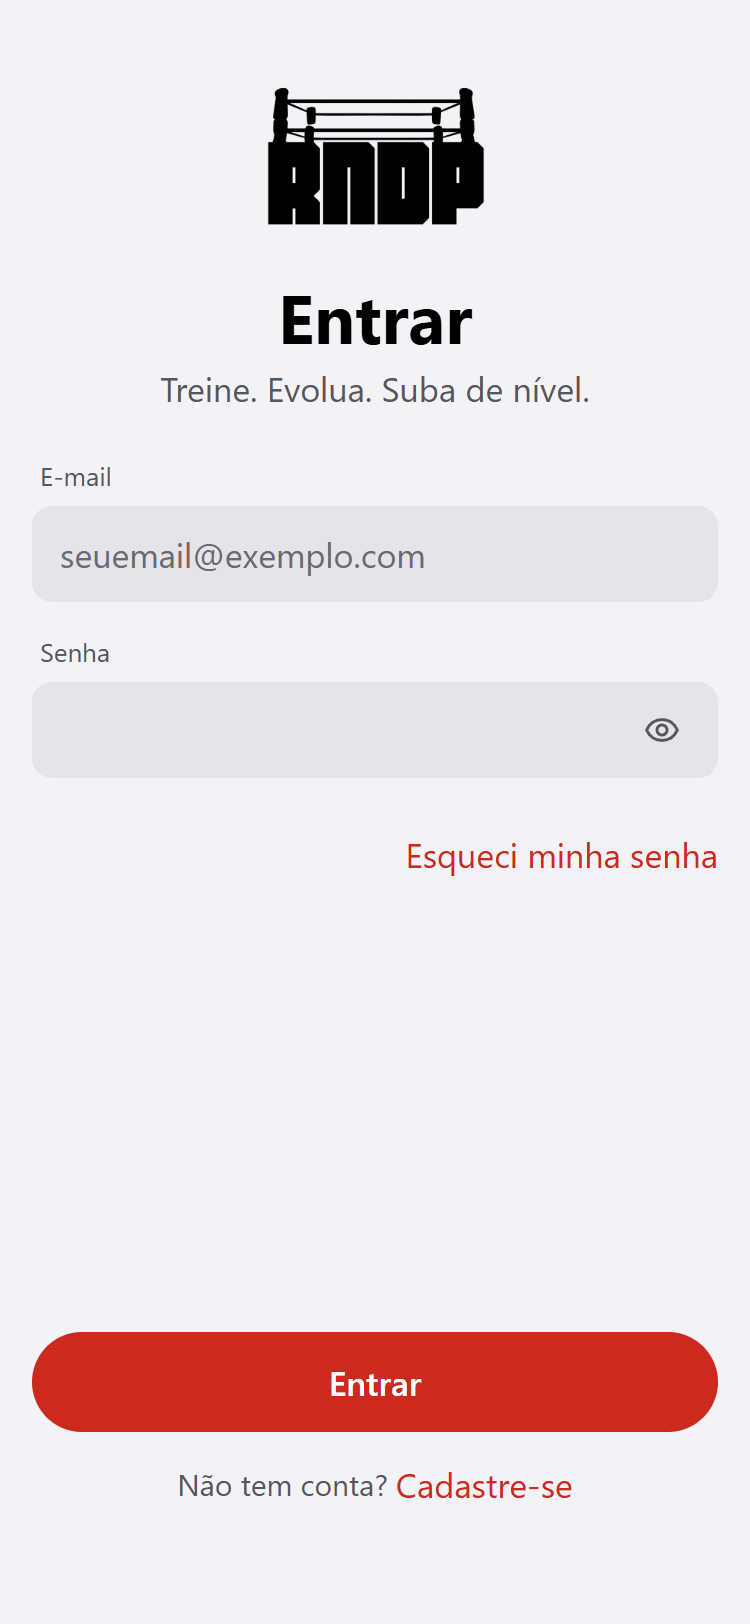
\includegraphics[width=0.27\textwidth]{figuras/tela-login.png}} &
    \fbox{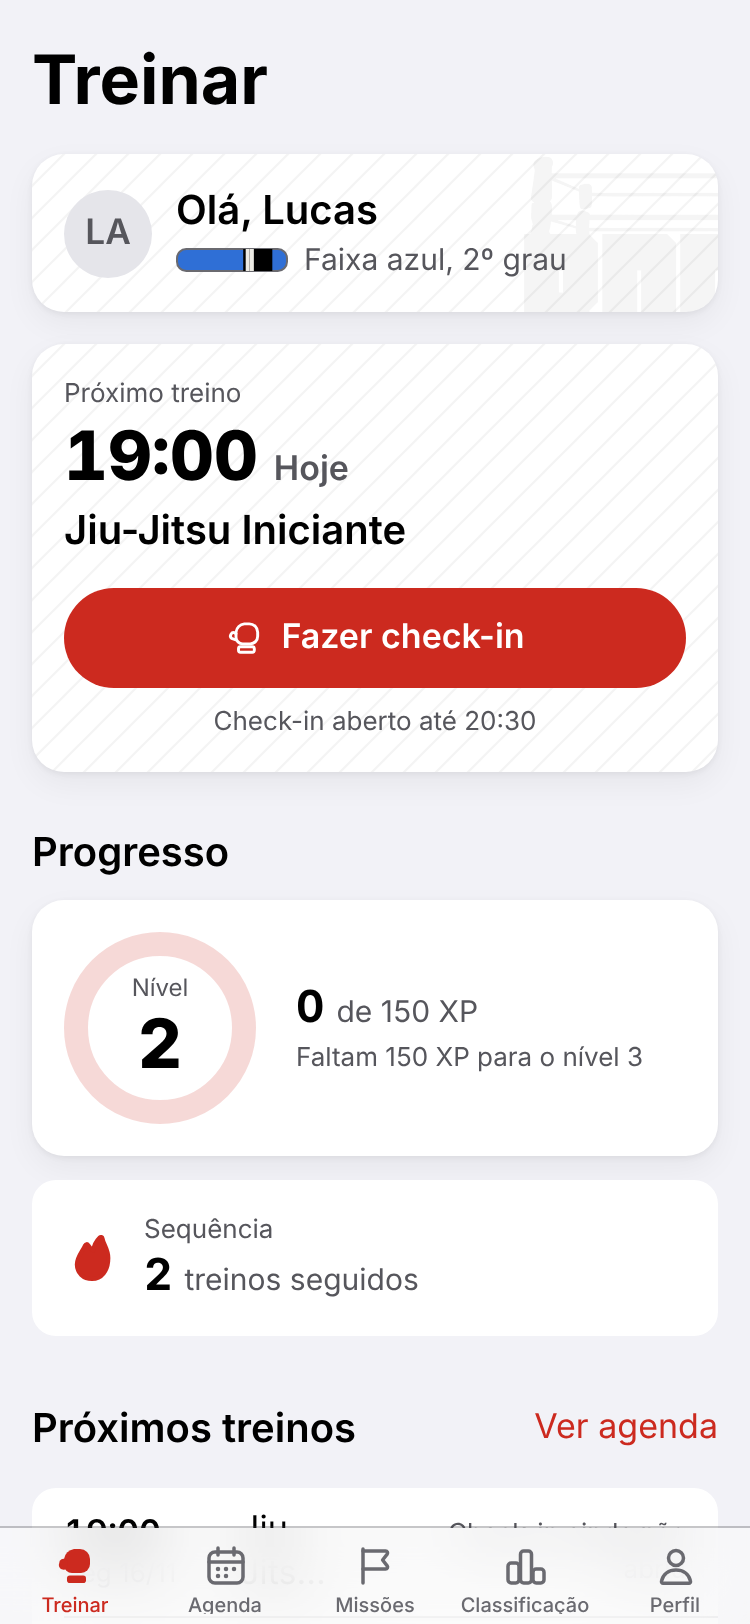
\includegraphics[width=0.27\textwidth]{figuras/tela-aluno-inicio.png}} &
    \fbox{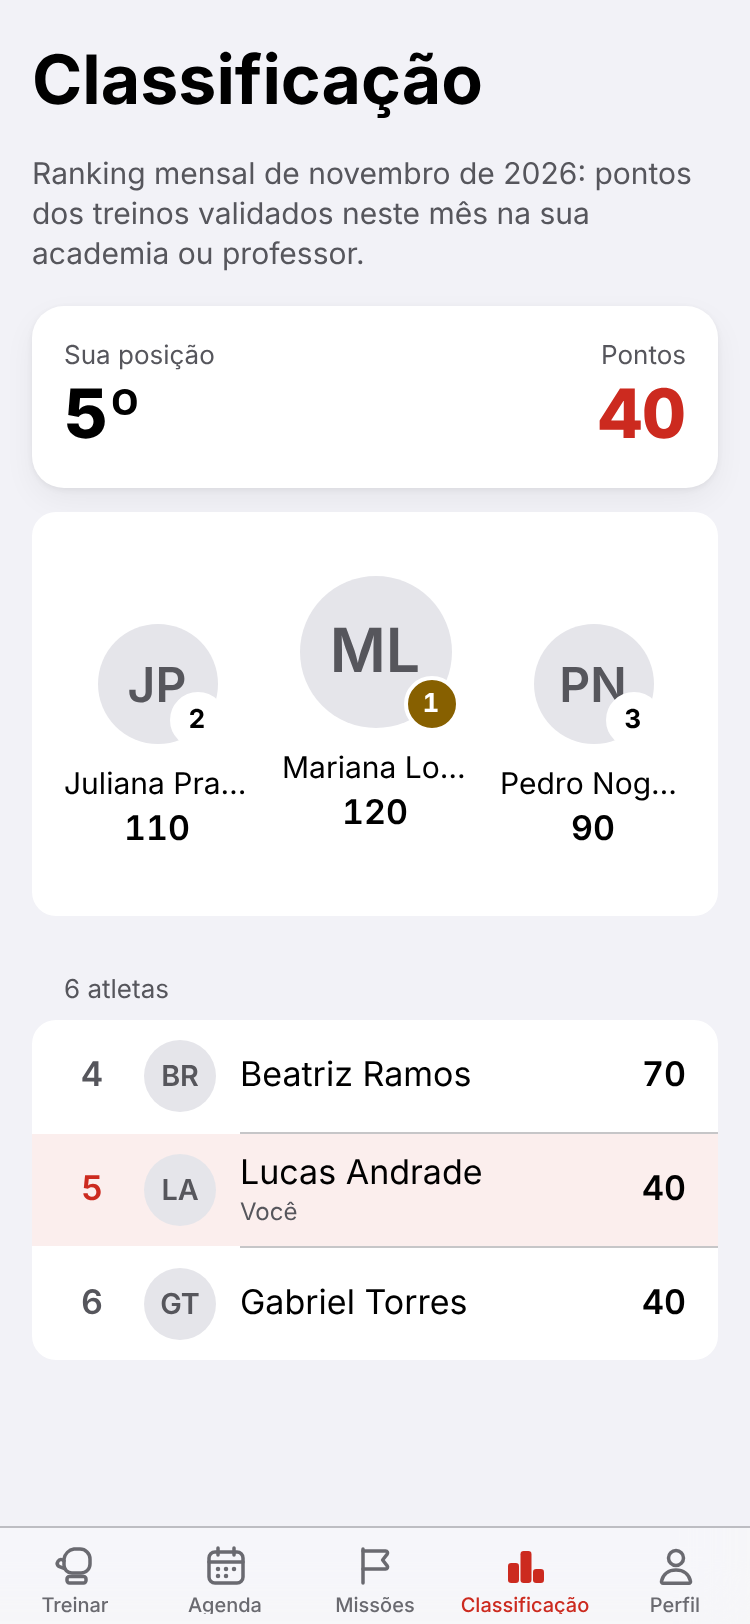
\includegraphics[width=0.27\textwidth]{figuras/tela-aluno-classificacao.png}} \\
    \footnotesize (a) & \footnotesize (b) & \footnotesize (c) \\[6pt]
    \fbox{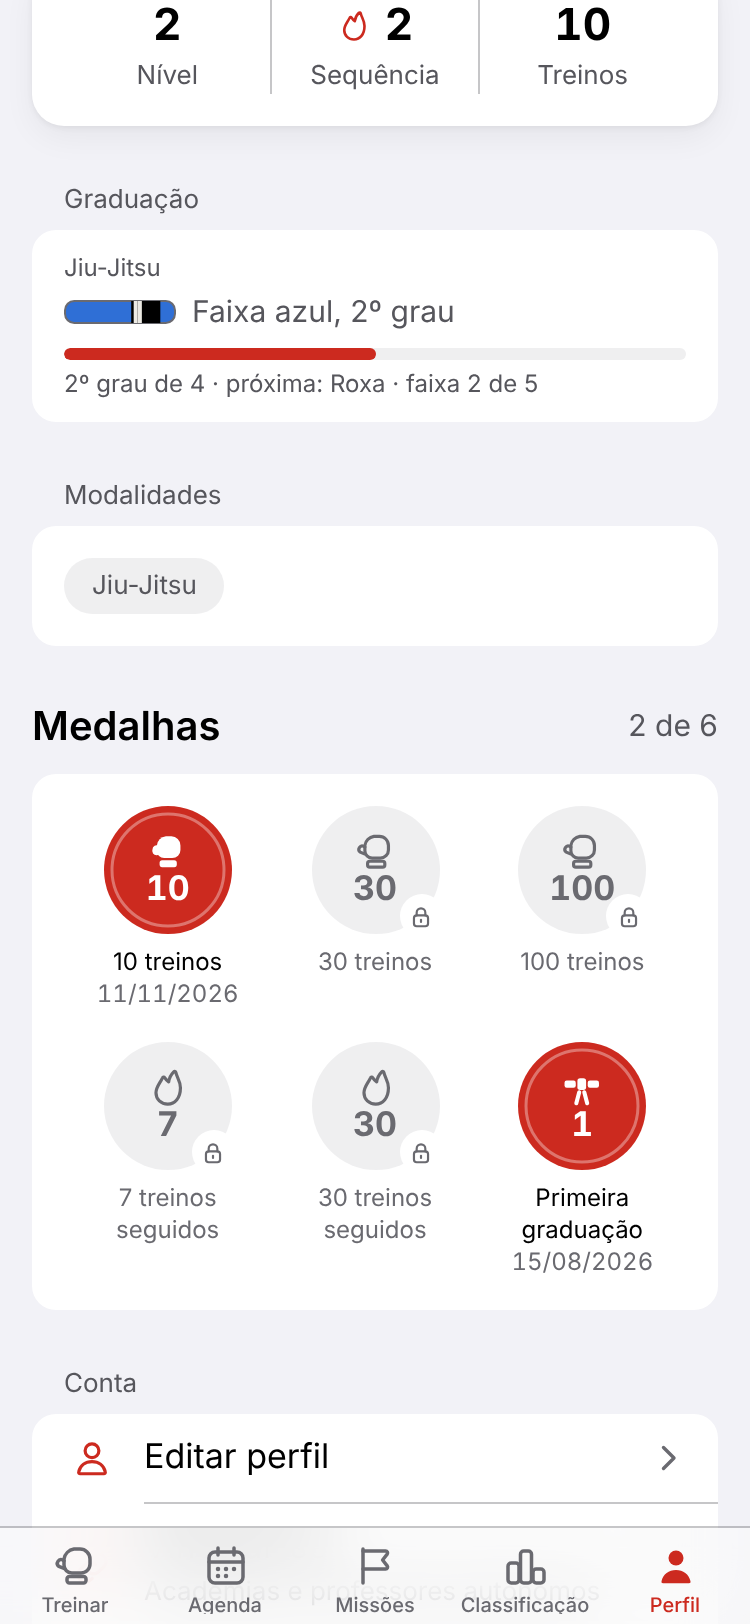
\includegraphics[width=0.27\textwidth]{figuras/tela-aluno-perfil.png}} &
    \fbox{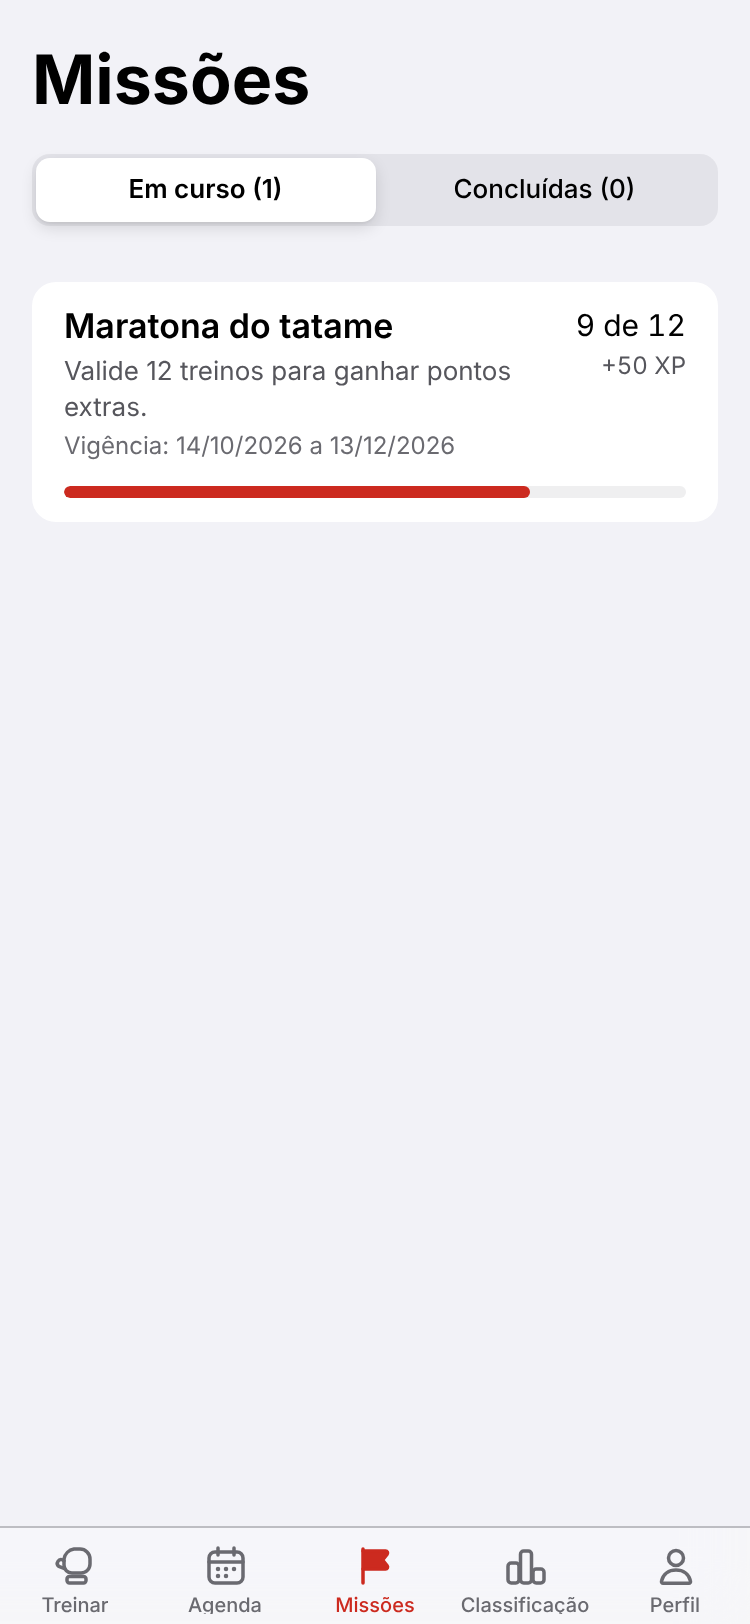
\includegraphics[width=0.27\textwidth]{figuras/tela-aluno-missoes.png}} &
    \fbox{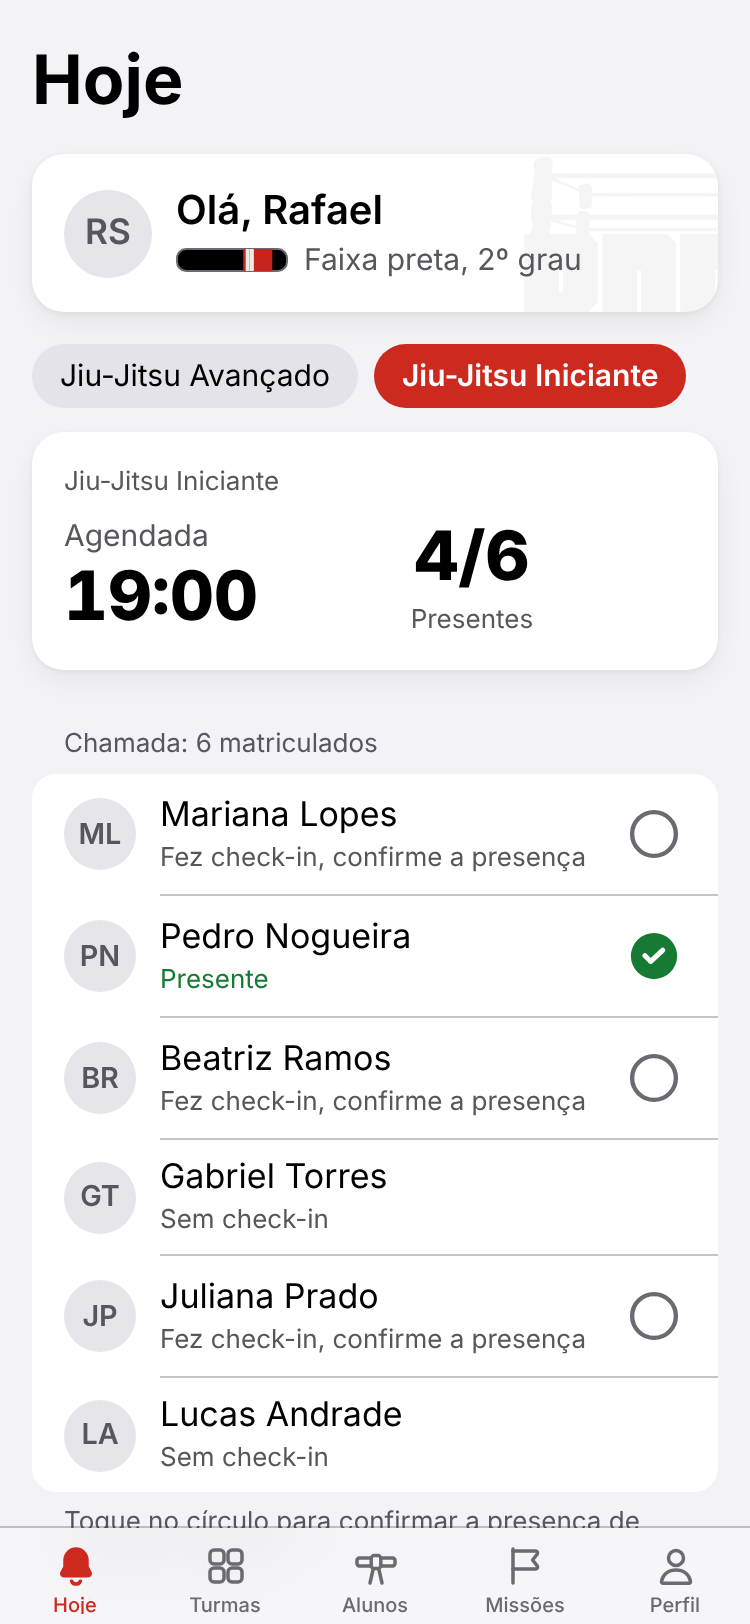
\includegraphics[width=0.27\textwidth]{figuras/tela-professor-chamada.png}} \\
    \footnotesize (d) & \footnotesize (e) & \footnotesize (f)
  \end{tabular}
  \fonte{Elaborado pelo autor (2026). Tema claro; as telas (b) a (f) foram
         capturadas na versão web, com dados fictícios.}
\end{figure}

Na tela inicial do aluno (b), o cartão do próximo treino traz o botão de
\textit{check-in} a um toque de distância, o que atende ao RNF01; logo
abaixo aparecem o anel de progresso, com o nível e o XP que falta para o
próximo, e a sequência de treinos. Na classificação (c), o aluno vê a sua
posição no mês e a linha dele aparece destacada. No perfil (d), a barra
de graduação mostra o grau atual dentro da faixa e a próxima faixa da
estrutura do responsável (RF33), e as medalhas conquistadas exibem a data
da conquista (RF19). Nas missões (e), cada missão mostra o progresso, a
recompensa e o período de vigência (RF23). Na chamada do professor (f),
cada aluno que fez \textit{check-in} tem a presença confirmada com um
toque no círculo.

\section{Situação de implementação dos requisitos}
\label{sec:situacao-implementacao}

O \autoref{qua:implementacao} resume o que foi implementado. As
limitações remanescentes foram registradas no repositório como decisões
pendentes, para que fiquem explícitas, e não escondidas na interface. O
critério de compatibilidade do RNF05 foi revisado de iOS 14 para iOS
16.4, versão mínima exigida pelo Expo SDK 58, adotado na etapa final; no
Android, o mínimo do SDK (Android 7.0) já atende ao critério original.

\begin{quadro}[!htb]
  \caption{Situação de implementação dos requisitos}
  \label{qua:implementacao}
  \centering
  \footnotesize
  \begin{tabular}{|p{2.2cm}|p{4.2cm}|p{7.0cm}|}
    \hline
    \textbf{Situação} & \textbf{Requisitos} & \textbf{Observação} \\ \hline
            Implementado & RF01--RF33; RN01--RN09; RNF01--RNF05, RNF07--RNF11 & Funcionalidades disponíveis nas telas e cobertas, na parte de segurança e de servidor, por testes em emulador. RF19, RF23, RF31 e RF33 também foram verificados em um iPhone, e o tempo de carregamento (RNF02) foi medido em 4G (\autoref{sec:testes-prototipo}). \\ \hline
    Não implementado & RNF06 & Decisão de projeto: o \textit{check-in} e a validação de presença são gravados em transações que exigem conexão, porque o servidor precisa garantir a janela de horário (RN08) e o limite de um \textit{check-in} por sessão (RN02). Um registro feito sem conexão poderia ser recusado depois, quando o aluno já acreditasse ter treinado com pontos garantidos. \\ \hline
  \end{tabular}
  \fonte{Elaborado pelo autor (2026), a partir do repositório do projeto.}
\end{quadro}

Os valores de gamificação têm um padrão, usado quando o professor ou a
academia não configuram os seus: 10 pontos por presença validada, dez
níveis com limiares crescentes (100, 250, 450\ldots{} até 3.250 pontos) e
medalhas para 10, 30 e 100 treinos, para sequências de 7 e 30 sessões e
para a primeira graduação. Esses valores permitiram construir e testar a
interface, mas ainda precisam ser calibrados com uso real.

Na conclusão dos requisitos que estavam parciais, quatro decisões
merecem registro:

\begin{itemize}
  \item \textbf{Medalhas (RF19).} Cada medalha é gravada em
        \texttt{usuarios/\{aluno\}/medalhas}, com a data de conquista,
        somente por Cloud Function; o aplicativo não consegue escrevê-la.
        O estorno de um \textit{check-in} não retira uma medalha já
        conquistada, e um \textit{script} de migração reconstruiu, a partir
        do histórico, a data das medalhas dos alunos existentes.
  \item \textbf{Missões (RF23).} O gestor define o público (todos os alunos
        vinculados, uma turma ou alunos escolhidos) e a vigência. A regra
        vale no banco de dados, não só na tela: só o público lê a missão,
        a conclusão manual só é aceita dentro da vigência, o progresso
        automático só conta treinos do período e o aviso de nova missão
        (RF31) vai só para o público, uma vez por aluno. Depois do fim da
        vigência, a missão continua no histórico de quem a concluiu.
  \item \textbf{Faixas (RF33).} O gestor personaliza, por modalidade, a
        ordem, o nome, a cor e o número de graus de cada faixa; sem
        personalização, vale a lista anterior como padrão. O registro de
        graduação (RF25) passou a gravar a faixa de forma estruturada, e o
        perfil do aluno ganhou a barra de progresso até a próxima
        graduação, medida pelos graus da faixa atual (por exemplo, ``2º
        grau de 4 · próxima: Roxa''). Graduações antigas, registradas como
        texto livre, foram convertidas por um \textit{script} que reconhece
        o nome da faixa; os textos sem correspondência permanecem como
        texto.
  \item \textbf{Notificações (RF31).} O projeto foi preparado para gerar
        versões instaláveis pelo EAS, e a tela de preferências de
        notificação ganhou botões para enviar uma notificação de teste ao
        próprio aparelho, o que permitiu validar o envio em um iPhone.
\end{itemize}

\section{Detalhes de implementação}

\subsection{Crédito de pontos com validação humana}

O \autoref{cod:validar} mostra o núcleo da função que confirma uma
presença. A confirmação e o crédito acontecem em uma única transação: o
\textit{check-in} recebe os pontos configurados pelo responsável e a
classificação do aluno, no escopo daquele responsável e no mês da sessão,
é atualizada. Se o professor desfizer a confirmação, os pontos são
estornados. A regra de segurança confere o \textit{check-in} e a
classificação na mesma transação: o crédito só pode ser o valor
configurado, e o estorno só pode devolver o que o \textit{check-in}
recebeu. Isso impede créditos arbitrários mesmo que alguém altere o
aplicativo.

\begin{codigo}[!htb]
  \caption{Validação de presença e crédito de pontos (TypeScript, trecho)}
  \label{cod:validar}
\begin{lstlisting}
await runTransaction(db, async (transacao) => {
  const checkin = (await transacao.get(checkinRef)).data() as CheckIn;
  const vaiCreditar = novoStatus === 'validado' && checkin.pontos === 0;
  const vaiEstornar = novoStatus === 'pendente' && checkin.pontos > 0;
  const periodo = periodoDe(checkin.dataHora.toDate());          // AAAA-MM
  const classificacaoId = vaiEstornar && checkin.classificacaoId
    ? checkin.classificacaoId
    : `${checkin.alunoId}_${checkin.responsavelId}_${periodo}`;
  const classificacaoRef = doc(db, 'classificacoes', classificacaoId);
  let pontosAtuais = 0, pontosDoCheckin = 0;
  if (vaiCreditar || vaiEstornar) {
    const snap = await transacao.get(classificacaoRef);
    pontosAtuais = snap.exists() ? snap.data().pontos : 0;
  }
  if (vaiCreditar) {                    // valor configurado ou padrao (RF33)
    const config = await transacao.get(doc(db, 'configuracoesGamificacao',
                                           checkin.responsavelId));
    pontosDoCheckin = config.exists() ? config.data().pontosPorCheckin
                                      : XP_POR_CHECKIN_VALIDADO;
  }
  transacao.update(checkinRef, {
    status: novoStatus, validadoPor: responsavelId,
    pontos: vaiCreditar ? pontosDoCheckin : vaiEstornar ? 0 : checkin.pontos,
    ...(vaiCreditar || vaiEstornar ? { classificacaoId } : {}),
  });
  if (vaiCreditar || vaiEstornar) {
    const delta = vaiCreditar ? pontosDoCheckin : -checkin.pontos;
    transacao.set(classificacaoRef, { pontos: pontosAtuais + delta,
      periodo: classificacaoId.slice(-7), origemCheckinId: checkinId },
      { merge: true });
  }
});
\end{lstlisting}

  \fonte{Elaborado pelo autor (2026), adaptado de \texttt{src/services/checkins.ts}.}
\end{codigo}

\subsection{Cálculo da sequência de treinos}

A sequência (RF21) conta as \textbf{sessões consecutivas} das turmas do
aluno em que ele teve presença validada, da mais recente para a mais
antiga (\autoref{cod:sequencia}). Sessões canceladas não contam, e uma
sessão com a janela de \textit{check-in} ainda aberta, ou com
\textit{check-in} aguardando validação, é ignorada, para não interromper a
sequência antes da hora. Assim, um dia sem aula não quebra a sequência:
ela só é interrompida quando houve sessão e o aluno não compareceu. O
mesmo critério é usado no aplicativo e nas Cloud Functions que avaliam as
missões de sequência.

\begin{codigo}[!htb]
  \caption{Cálculo da sequência de treinos por sessão (TypeScript)}
  \label{cod:sequencia}
\begin{lstlisting}
export function calcularSequencia(sessoes: Sessao[], checkins: CheckIn[],
                                  agora: Date = new Date()): number {
  const statusPorSessao = new Map(checkins.map((c) => [c.sessaoId, c.status]));
  const maisRecentesPrimeiro = sessoes
    .filter((s) => s.status !== 'cancelada')
    .sort((a, b) => b.janelaCheckInFim.toMillis() - a.janelaCheckInFim.toMillis());
  let sequencia = 0;
  for (const sessao of maisRecentesPrimeiro) {
    const status = statusPorSessao.get(sessao.id);
    if (status === 'validado') sequencia += 1;
    else if (sessao.janelaCheckInFim.toDate() > agora || status === 'pendente') continue;
    else break;                         // houve sessao e o aluno nao foi
  }
  return sequencia;
}
\end{lstlisting}
  \fonte{Elaborado pelo autor (2026), adaptado de \texttt{src/utils/gamificacao.ts}.}
\end{codigo}


  % =====================================================================
%  CAPÍTULO 5 -- PROCEDIMENTOS DE TESTES E VALIDAÇÃO
%  (Regulamento, Art. 9º, item v)
% ---------------------------------------------------------------------
%  Em linguagem simples:
%   - TESTAR  = verificar se o aplicativo foi construído CORRETAMENTE
%               (faz o que foi especificado, sem falhas?).
%   - VALIDAR = verificar se foi construído o aplicativo CERTO
%               (as ideias resolvem o problema do usuário?).
%  Num projeto de ideação, a VALIDAÇÃO DAS IDEIAS vem antes e acontece
%  em paralelo à construção. Por isso este capítulo começa por ela.
%
%  A tabela de notas (tab-survey.tex) e a figura do survey são GERADAS
%  pelo script scripts/analise_survey.py. Se os dados mudarem, rode o
%  script de novo em vez de editar os números à mão.
% =====================================================================

\chapter{Procedimentos de testes e validação}
\label{cap:testes}

A avaliação do RoundUp ocorreu em três frentes: (i) a avaliação das
ideias por usuários reais, por meio de um questionário; (ii) o teste do
questionário e do procedimento de análise com respostas sintéticas; e
(iii) os testes do protótipo em relação aos requisitos. Apenas a primeira
frente \textbf{valida as ideias}, isto é, verifica se as funcionalidades
propostas fazem sentido para o público; as outras duas \textbf{testam}
instrumentos e software, verificando se fazem o que foi especificado.

\section{Avaliação das ideias com usuários reais}
\label{sec:val-survey}

\subsection{Instrumento e aplicação}

O questionário foi elaborado no Google Forms, com termo de consentimento
na primeira página, e recebeu respostas em 18 e 19 de setembro de 2026.
Após as perguntas de perfil, o respondente era encaminhado a uma de três
seções, conforme sua relação atual com as lutas: \textbf{professor},
\textbf{praticante} (treina atualmente) ou \textbf{ex-praticante} (já
treinou, mas parou). Cada seção combinava:

\begin{itemize}
  \item perguntas sobre motivação, evasão e acompanhamento dos treinos;
  \item a avaliação de cada ideia do \autoref{qua:ideias}, convertida em
        recurso do aplicativo, em uma escala de 1 (pouco útil) a 5 (muito
        útil);
  \item perguntas abertas sobre funcionalidades desejadas e motivos para
        abandonar o aplicativo.
\end{itemize}

Nem todas as ideias foram apresentadas a todos os perfis: o alerta de
ausência (I12) foi apresentado a professores e ex-praticantes, e o
relatório da turma (I13), apenas a professores. As perguntas completas
estão no \autoref{ap:questionario}.

O link do questionário foi divulgado por WhatsApp, em conversas e grupos
do círculo de contatos do autor. Essa forma de divulgação explica o perfil
da amostra: como o autor pratica Jiu-Jitsu, todos os respondentes vieram
dessa modalidade, e nenhum professor foi alcançado.

\subsection{Perfil dos respondentes}

Foram obtidas \textbf{seis respostas}: quatro de praticantes e duas de
ex-praticantes. \textbf{Nenhum professor respondeu}, o que impede avaliar,
com usuários reais, as ideias voltadas à gestão. A \autoref{tab:perfil}
resume o perfil da amostra. Os dados pessoais de contato informados por
alguns respondentes foram descartados da análise.

\begin{table}[!htb]
  \centering
  \caption{Perfil dos respondentes do questionário}
  \label{tab:perfil}
  \footnotesize
  \begin{tabular}{lcc}
    \toprule
    \textbf{Característica} & \textbf{Praticantes} & \textbf{Ex-praticantes} \\
    \midrule
    Respondentes                    & 4 & 2 \\
    Gênero feminino / masculino     & 2 / 2 & 0 / 2 \\
    Menos de 18 anos                & 1 & 0 \\
    18 a 34 anos                    & 0 & 2 \\
    35 a 44 anos                    & 3 & 0 \\
    Pratica(va) Jiu-Jitsu           & 4 & 2 \\
    Treina(ou) há mais de 3 anos    & 3 & 2 \\
    \bottomrule
  \end{tabular}
  \fonte{Dados da pesquisa (2026).}
\end{table}

\subsection{Como os dados foram analisados}

Com apenas seis respostas, não faz sentido usar testes estatísticos para
afirmar que uma ideia é ``melhor'' que outra: qualquer diferença pode ser
fruto do acaso. Por isso, a análise é \textbf{descritiva}. Para cada
ideia foram calculadas duas medidas:

\begin{itemize}
  \item a \textbf{média}: soma das notas dividida pelo número de notas. É
        fácil de interpretar, mas muda bastante quando uma única pessoa
        dá notas muito altas ou muito baixas;
  \item a \textbf{mediana}: o valor do meio quando as notas são
        colocadas em ordem. Ela é menos afetada por respostas extremas e,
        por isso, ajuda a conferir se a média está ``puxada'' por alguém.
\end{itemize}

Por exemplo, se três pessoas dão as notas 1, 4 e 5, a média é 3,3, mas a
mediana é 4: a nota 1 puxa a média para baixo, enquanto a mediana mostra
que a maioria avaliou bem.

\subsection{Resultados quantitativos}

A \autoref{tab:survey-notas} apresenta as notas atribuídas a cada ideia.

\begin{table}[!htb]
  \centering
  \caption{Notas atribuídas às ideias (escala de 1 a 5)}
  \label{tab:survey-notas}
  \footnotesize
  \begin{tabular}{clccccc}
    \toprule
    & & \multicolumn{3}{c}{\textbf{Média}} & & \\
    \cmidrule(lr){3-5}
    \textbf{ID} & \textbf{Ideia} & \textbf{Prat.} & \textbf{Ex-prat.} & \textbf{Geral} & \textbf{Mediana} & \textbf{n} \\
    \midrule
% Gerado por scripts/analise_survey.py -- nao edite a mao
    I01 & Pontos de experiência (XP) & 3,5 & 4,0 & 3,7 & 4,0 & 6 \\
    I02 & Check-in de presença & 3,5 & 2,5 & 3,2 & 3,5 & 6 \\
    I03 & Contador de frequência & 3,0 & 4,0 & 3,3 & 4,0 & 6 \\
    I04 & Ofensiva (sequência) & 3,5 & 4,0 & 3,7 & 4,0 & 6 \\
    I05 & Missões e desafios semanais & 3,5 & 2,5 & 3,2 & 3,5 & 6 \\
    I06 & Ranking de frequência & 3,5 & 4,0 & 3,7 & 4,0 & 6 \\
    I07 & Medalhas por marcos & 3,5 & 4,0 & 3,7 & 4,0 & 6 \\
    I08 & Barra de progresso da graduação & 3,8 & 4,0 & 3,8 & 4,0 & 6 \\
    I09 & Histórico de presença e evolução & 4,0 & 3,5 & 3,8 & 4,0 & 6 \\
    I10 & Mural/feed da turma & 3,8 & 2,5 & 3,3 & 4,0 & 6 \\
    I11 & Lembretes nos dias de treino & 3,2 & 2,5 & 3,0 & 3,5 & 6 \\
    I12 & Alerta/mensagem após ausência & -- & 2,5 & 2,5 & 2,5 & 2 \\
    I13 & Relatório da turma (professor) & -- & -- & -- & -- & 0 \\
    \bottomrule
% (inclui o \bottomrule)
  \end{tabular}
  \fonte{Dados da pesquisa (2026). Prat. = praticantes (n = 4);
         Ex-prat. = ex-praticantes (n = 2); ``--'' = ideia não apresentada ao perfil.}
\end{table}

De modo geral, as ideias receberam avaliação moderadamente positiva: onze
das doze ideias avaliadas têm mediana igual ou superior a 3,5. As mais
bem avaliadas foram a \textbf{barra de progresso até a próxima
graduação} (I08) e o \textbf{histórico de presença e evolução} (I09),
ambas com média 3,8 -- coerentes com o eixo ``progresso visível'' da
literatura sobre gamificação. As menos bem avaliadas foram a mensagem
automática após ausência (I12, média 2,5, avaliada apenas pelos dois
ex-praticantes), os lembretes (I11, média 3,0), o \textit{check-in}
(I02) e as missões semanais (I05), ambos com média 3,2.

Dois cuidados são necessários na leitura desses números. Primeiro, as
respostas foram muito heterogêneas: uma respondente atribuiu nota máxima
a todas as ideias, e outro atribuiu notas 1 ou 2 à maioria delas. Com
seis pessoas, cada uma dessas respostas desloca bastante as médias.
Segundo, as diferenças entre ideias são pequenas (quase todas entre 3,0
e 3,8) e não devem ser lidas como uma classificação definitiva.

\subsection{Resultados qualitativos}

As respostas abertas e de múltipla escolha trouxeram indícios que não
aparecem nas notas:

\begin{itemize}
  \item \textbf{Motivação}: todos os praticantes apontaram a saúde mental
        e o alívio do estresse como motivo para continuar treinando; três
        de quatro citaram também a saúde física e o convívio com a turma.
  \item \textbf{Frequência}: nenhum praticante registra a própria
        frequência (dois acompanham ``só mentalmente'' e dois não
        acompanham), e dois deles apontaram a frequência como a
        informação que hoje ``se perde''. Isso reforça RF15 e RF24.
  \item \textbf{Graduação}: o praticante com menos tempo de treino (3 a 6
        meses) declarou não fazer ideia do que precisa para a próxima
        graduação, justamente a fase em que a evasão tende a ser maior.
        Isso reforça RF17 e RF25.
  \item \textbf{Evasão}: os dois ex-praticantes pararam por falta de tempo
        ou conflito com a rotina; ambos foram procurados pelo professor e
        ambos afirmaram que o aplicativo não teria mudado sua decisão.
        Isso sugere um limite importante: parte da evasão tem causas
        externas que um aplicativo não resolve.
  \item \textbf{Riscos de abandono do aplicativo}: os respondentes citaram
        ``muitas notificações'' e ``inserir muitos dados constantemente''.
        Esses comentários reforçaram o RNF01 (\textit{check-in} em até três
        toques) e levaram a tornar as notificações configuráveis por tipo
        (RF31).
  \item \textbf{Privacidade}: a disposição a usar o aplicativo caso os
        dados ficassem visíveis apenas para o aluno e o professor variou
        de 1 a 4, o que reforçou a adesão opcional à classificação (RNF11)
        e a decisão de não incorporar o mural da turma.
\end{itemize}

\section{Teste do instrumento com respostas sintéticas}
\label{sec:val-personas}

Como a coleta real teve seis respostas e nenhuma de professor, parte do
questionário, incluindo toda a seção do professor e as ideias I12 e I13,
nunca havia sido processada. Para testar o formulário e o procedimento de
análise sem misturar dados sintéticos com a coleta real, foram geradas
\textbf{65 respostas sintéticas} a partir de personas. Esta seção
descreve como elas foram produzidas e o que o teste verificou.

\subsection{Personas e geração das respostas}

Foram construídas \textbf{12 personas sintéticas}: seis alunos ativos,
quatro ex-alunos e dois professores, um deles dono de academia,
distribuídos pelas faixas etárias do próprio formulário. As fichas, que estão
no repositório do projeto (\autoref{ap:artefatos}), descrevem idade, modalidade, rotina, motivações,
riscos de evasão e postura diante da gamificação, e trazem respostas-modelo
ao questionário. Elas foram escritas a partir do padrão observado nas seis
respostas reais, como respostas abertas curtas, recusas de uma palavra,
acentos faltando e três padrões de uso da escala (notas iguais em tudo,
variação estreita e discriminação forte).

As respostas foram geradas por um \textit{script} em Python, escrito com
apoio do Claude (Anthropic, identificador \texttt{claude-opus-5-5}) em
26 de outubro de 2026. O \textit{script} combina bancos de respostas
curtas por pergunta com regras por perfil e faixa etária, e sorteia as
combinações com semente fixa (\texttt{random.seed(26102026)}), o que
torna a geração reproduzível. \textbf{Não houve um \textit{prompt} por
resposta}: as 12 fichas orientaram as regras, e as 65 linhas não
correspondem uma a uma às fichas. A \autoref{tab:perfil-personas} mostra
a distribuição resultante, definida para cobrir os perfis ausentes da
amostra real; entre os dez professores, quatro são donos de academia, e
os ex-alunos têm doze motivos principais de abandono diferentes.

\begin{table}[!htb]
  \centering
  \caption{Perfil das respostas sintéticas}
  \label{tab:perfil-personas}
  \footnotesize
  \begin{tabular}{lccc}
    \toprule
    \textbf{Característica} & \textbf{Alunos ativos} & \textbf{Ex-alunos} & \textbf{Professores} \\
    \midrule
    Respostas                           & 32 & 23 & 10 \\
    Gênero feminino / masculino         & 8 / 24 & 8 / 14 & 1 / 9 \\
    Menos de 18 anos                    & 8 & 2 & 0 \\
    18 a 24 anos                        & 9 & 6 & 0 \\
    25 a 34 anos                        & 6 & 6 & 3 \\
    35 a 44 anos                        & 6 & 5 & 3 \\
    45 anos ou mais                     & 3 & 4 & 4 \\
    Jiu-Jitsu / outras modalidades      & 11 / 21 & 12 / 11 & 6 / 4 \\
    \bottomrule
  \end{tabular}
  \fonte{Elaborado pelo autor (2026). Uma resposta de ex-aluno não
         informa o gênero. As outras modalidades incluem Boxe, Muay Thai,
         Judô, Taekwondo, Karatê e MMA.}
\end{table}

O envio foi feito por Google Apps Script, no editor de uma
\textbf{cópia} do formulário (``RoundUp (Personas IA)''), sem planilha de
respostas vinculada à pesquisa: cada resposta foi primeiro validada contra
as alternativas do formulário e depois registrada pela API do Google
Forms, sem passar pelo link público. As 65 respostas foram enviadas em 26
de outubro de 2026, entre 13h12 e 13h14, cada uma com o marcador
\texttt{sintetico-<ID>} no campo de contato (A01 a A32 para alunos, E01 a
E23 para ex-alunos e P01 a P10 para professores). A conferência da
exportação confirmou as 65 respostas com o marcador e nenhuma resposta
sintética na base da pesquisa real.

\subsection{O que o teste verificou}

O teste confirmou que:

\begin{itemize}
  \item o formulário aceita as combinações de alternativas previstas, já
        que todas as 65 respostas passaram pela validação contra as
        alternativas antes do registro;
  \item o roteamento por perfil leva às três seções, inclusive a do
        professor, que nunca havia recebido respostas, com os itens das
        ideias I12 e I13;
  \item o procedimento de análise (\texttt{scripts/analise\_personas.py})
        lê a exportação do formulário, identifica as colunas de cada perfil,
        trata variações de acento e espaços e gera as tabelas desta seção.
        O mesmo procedimento poderá ser usado em uma nova coleta real que
        inclua professores;
  \item os dois conjuntos de dados ficaram separados: as respostas
        sintéticas não entraram na \autoref{tab:survey-notas} nem nas
        decisões sobre os requisitos.
\end{itemize}

\subsection{Resultados descritivos do teste}

A \autoref{tab:personas-comparacao} apresenta as médias das respostas
sintéticas ao lado das médias reais. Ela é mostrada apenas para documentar
a saída da análise e verificar o gerador: \textbf{os valores sintéticos
refletem as regras escritas pelo autor e pelo modelo, e não a percepção de
usuários}.

\begin{table}[!htb]
  \centering
  \caption{Notas médias das respostas sintéticas e das respostas reais}
  \label{tab:personas-comparacao}
  \footnotesize
  \begin{tabular}{clcccccc}
    \toprule
    & & \multicolumn{3}{c}{\textbf{Sintéticas}} & \multicolumn{2}{c}{\textbf{Alunos e ex-alunos}} & \\
    \cmidrule(lr){3-5}\cmidrule(lr){6-7}
    \textbf{ID} & \textbf{Ideia} & \textbf{Alunos} & \textbf{Ex-al.} & \textbf{Prof.} & \textbf{Sintét.} & \textbf{Reais} & \textbf{Dif.} \\
    \midrule
% Gerado por scripts/analise_personas.py -- nao edite a mao
    I01 & Pontos de experiência (XP) & 3,7 & 4,0 & 4,1 & 3,8 & 3,7 & +0,2 \\
    I02 & Check-in de presença & 4,2 & 4,0 & 5,0 & 4,1 & 3,2 & +0,9 \\
    I03 & Contador de frequência & 3,8 & 4,0 & 4,8 & 3,9 & 3,3 & +0,6 \\
    I04 & Ofensiva (sequência) & 3,9 & 4,1 & -- & 4,0 & 3,7 & +0,3 \\
    I05 & Missões e desafios semanais & 4,1 & 4,2 & 2,5 & 4,1 & 3,2 & +0,9 \\
    I06 & Ranking de frequência & 3,4 & 3,5 & 2,4 & 3,4 & 3,7 & $-$0,2 \\
    I07 & Medalhas por marcos & 3,8 & 4,0 & 3,5 & 3,9 & 3,7 & +0,2 \\
    I08 & Barra de progresso da graduação & 4,1 & 4,0 & 4,5 & 4,1 & 3,8 & +0,2 \\
    I09 & Histórico de presença e evolução & 4,1 & 4,0 & -- & 4,0 & 3,8 & +0,2 \\
    I10 & Mural/feed da turma & 3,6 & 3,2 & -- & 3,4 & 3,3 & +0,1 \\
    I11 & Lembretes nos dias de treino & 3,2 & 3,4 & -- & 3,3 & 3,0 & +0,3 \\
    I12 & Alerta/mensagem após ausência & -- & 3,6 & 5,0 & 3,6 & 2,5 & +1,1 \\
    I13 & Relatório da turma (professor) & -- & -- & 4,5 & -- & -- & -- \\
    \bottomrule
% (inclui o \bottomrule)
  \end{tabular}
  \fonte{Elaborado pelo autor (2026). Sintéticas: 32 alunos, 23 ex-alunos,
         10 professores; reais: 6. Dif. = sintéticas menos reais. ``--'' =
         ideia não apresentada ao perfil.}
\end{table}

Nas ideias de progresso visível (I01, I04, I07, I08 e I09), as médias
sintéticas ficaram a no máximo 0,3 ponto das reais. Isso era esperado,
porque as regras do gerador foram escritas a partir das respostas reais, e
não confirma nada sobre as ideias; mostra apenas que o gerador reproduziu
o padrão que lhe deu origem. As maiores diferenças, no \textit{check-in}
(I02), nas missões (I05), no contador de frequência (I03) e no alerta após
ausência (I12), indicam onde as regras do gerador se afastaram dos dados
reais e devem ser recalibradas se ele for reutilizado. O gerador também produziu menos notas extremas do que os respondentes
reais, e as respostas abertas sintéticas repetem frases idênticas entre
linhas diferentes, efeito dos bancos de respostas que não seria esperado
de pessoas reais.

\subsection{Limitação}

As respostas sintéticas reproduzem padrões supostos pelo pesquisador e
pelo modelo de linguagem. Elas servem como insumo complementar da
ideação, para repensar os requisitos, e para testar o instrumento e a
análise, mas \textbf{não servem como evidência de validação das ideias
nem da percepção de usuários}
\cite{argyle2023,aher2023}. As respostas de professor e de dono de
academia são as mais frágeis, porque a base real não tinha nenhuma
resposta desse perfil: as dez linhas de professor derivam de apenas duas
fichas e funcionam como hipóteses a validar e como dados de teste da
seção do professor.

\section{Testes do protótipo}
\label{sec:testes-prototipo}

Os testes do protótipo verificam se o software faz o que foi
especificado. Eles foram organizados em três níveis: testes automatizados
de unidade, testes automatizados das regras de segurança e das funções
de servidor, executados em emulador local, e um roteiro de teste manual
da interface para o Ciclo 1.

\subsection{Testes automatizados}

A \autoref{tab:suites} resume as suítes de testes do repositório. Os
testes das regras de segurança são os mais importantes do projeto,
porque é nas regras que estão garantidas as regras de negócio que
protegem a credibilidade da gamificação (RN01, RN02 e RN08) e o
isolamento de dados (RNF04).

\begin{table}[!htb]
  \centering
  \caption{Suítes de testes automatizados}
  \label{tab:suites}
  \footnotesize
  \begin{tabular}{p{3.6cm}p{6.6cm}cc}
    \toprule
    \textbf{Suíte} & \textbf{O que verifica} & \textbf{Casos} & \textbf{Aprovados} \\
    \midrule
    Unidade (\texttt{src/utils}) & Datas e janelas de sessão, sequência, níveis e validação da configuração & 37 & 37 \\
    Regras do Firestore (\texttt{tests/rules}) & Usuários, vínculos, turmas, matrículas, sessões, \textit{check-ins}, classificação, missões, configuração, notificações e coleções bloqueadas & 124 & 124 \\
    Cloud Functions (\texttt{tests/functions}) & Leitores de sessões e classificações, progresso e pontos de missões, exclusão de conta, graduações e notificações & 33 & 33 \\
    \bottomrule
  \end{tabular}
  \fonte{Elaborado pelo autor (2026). Todas as suítes executadas em 12 nov. 2026.}
\end{table}

As três suítes foram executadas em 12 de novembro de 2026, sobre a versão entregue do código. Os testes de
regras e de Cloud Functions rodaram nos emuladores do Firebase
(\texttt{firebase-tools} 15.29.0), que exigem Java 21 ou superior; foi
usado o OpenJDK 22, e as funções rodaram no Node 21, embora o projeto
declare o Node 22. A suíte de Cloud Functions usa também os emuladores de
autenticação e de armazenamento, necessários para testar a exclusão de
conta. Todas as suítes passaram integralmente na versão final
do código, depois da correção descrita na
\autoref{sec:defeitos-testes}.

A \autoref{tab:testes} relaciona os principais casos de teste aos
requisitos.

\begin{table}[!htb]
  \centering
  \caption{Casos de teste do protótipo}
  \label{tab:testes}
  \footnotesize
  \begin{tabular}{ccp{6.0cm}p{3.2cm}}
    \toprule
    \textbf{Caso} & \textbf{Requisito} & \textbf{Descrição} & \textbf{Esperado} \\
    \midrule
    CT01 & RF13, RN08 & Aluno matriculado faz \textit{check-in} dentro da janela & Aceito \\
    CT02 & RN02 & Segundo \textit{check-in} na mesma sessão & Negado \\
    CT03 & RN08 & \textit{Check-in} antes da abertura ou depois do fim da janela & Negado \\
    CT04 & RN05 & \textit{Check-in} de aluno não matriculado & Negado \\
    CT05 & RN01 & Aluno tenta marcar o próprio \textit{check-in} como validado & Negado \\
    CT06 & RF22 & Responsável pela sessão valida o \textit{check-in} & Aceito \\
    CT07 & RF16, RN01 & Crédito do valor configurado e estorno do valor recebido & Aceito \\
    CT08 & RN01 & Alteração arbitrária de pontos na classificação & Negado \\
    CT09 & RNF04 & Aluno de outra turma tenta ler a sessão & Negado \\
    CT10 & RF11 & Matrícula nova inclui o aluno nas sessões futuras & Aluno incluído \\
    CT11 & RF28 & Alteração de consentimento LGPD já registrado & Negado \\
    CT12 & RF29 & Exclusão de conta apaga os dados do usuário e preserva os de outros & Aceito \\
    CT13 & RN09, RNF11 & Aluno lê a classificação de outro escopo ou de quem não participa & Negado \\
    CT14 & RF18 & Aluno grava o próprio progresso de missão & Negado \\
    CT15 & RNF01 & \textit{Check-in} a partir da tela inicial (roteiro manual) & $\leq$ 3 toques \\
    \bottomrule
  \end{tabular}
  \fonte{Elaborado pelo autor (2026), a partir de \texttt{tests/} e
         \texttt{docs/roteiro-teste-ciclo1.md}.}
\end{table}

Os casos CT01 a CT09, CT11, CT13 e CT14 correspondem a testes da suíte
de regras; o CT10 e o CT12, à suíte de Cloud Functions; e o CT15, ao
roteiro manual, segundo o
qual o \textit{check-in} exige dois toques na agenda e um toque na tela
inicial da versão final da interface.

\subsection{Verificações de qualidade da interface}

Na última rodada de refinamento da interface, o código passou pela
verificação de tipos do TypeScript em modo estrito sem erros, e nove
telas foram analisadas, nos temas claro e escuro, com a ferramenta de
acessibilidade axe-core (critérios WCAG 2.1, níveis A e AA), sem violações
registradas. As cores de texto foram ajustadas para atingir a razão
mínima de contraste de 4,5:1 nos dois temas; por isso, o vermelho de
destaque e os cinzas de texto ficaram um pouco mais escuros que os
padrões do iOS no tema claro. A interface foi conferida na versão web; o
comportamento exclusivo dos aparelhos, como as barras translúcidas, os
gestos das folhas e o retorno tátil, ainda precisa ser verificado em
dispositivo.

\subsection{Defeitos encontrados pelos testes}
\label{sec:defeitos-testes}

Os testes automatizados revelaram defeitos que não apareceriam em uma
avaliação apenas visual. O mais relevante foi a descoberta de que o
motor de regras do Firestore recusa consultas de lista cuja permissão
dependa de dados de outra coleção, o que levou às decisões de modelagem
da \autoref{sec:modelagem-estatica}. Também foi encontrado um caso em que
a gravação do vínculo e do documento privado, feita na mesma transação,
era negada porque a regra lia o estado anterior à transação; a correção
foi usar as funções que leem o estado posterior.

Na primeira execução da suíte de Cloud Functions, só um dos quatro testes
passou: os três que esperavam a sincronização de \texttt{leitoresIds} na
matrícula, no cancelamento e na reativação pararam pelo limite de tempo,
e o único aprovado era justamente o que espera que nada aconteça. A causa
era de configuração, e não de lógica: o emulador subia no projeto
padrão do Firebase (\texttt{roundup-app-a5a82}), enquanto os testes
gravavam no projeto de demonstração \texttt{demo-roundup-app}, de modo
que os gatilhos das funções escutavam o projeto errado. A correção
(\textit{commit} \texttt{6098f4e}) fixou o projeto
\texttt{demo-roundup-app} nos dois comandos de teste, o que também impede
o emulador de acessar o projeto de produção, e aumentou o limite de tempo
da suíte de 5 para 20 segundos, já que a espera dentro do teste pode
chegar a 10 segundos. Depois da correção, as quatro passaram.

  % =====================================================================
%  CAPÍTULO 6 -- RESULTADOS E CONSIDERAÇÕES FINAIS
%  (Regulamento, Art. 9º, item vi; Manual, seção 2.2.3)
%  O Manual recomenda que a parte conclusiva NÃO contenha citações.
% =====================================================================

\chapter{Resultados e considerações finais}
\label{cap:resultados}

Este projeto conduziu a concepção do RoundUp como um processo de
ideação, no qual as ideias de funcionalidades foram convertidas em
requisitos e esses requisitos foram usados, ao mesmo tempo, para
construir o aplicativo e para avaliar as ideias com usuários reais. Essa estratégia permitiu rastrear cada
funcionalidade desde a ideia até a decisão de mantê-la, ajustá-la ou
revisá-la, e daí até o código e os testes.

\section{Resultados alcançados}

Os objetivos específicos apresentados no \autoref{cap:introducao} foram
atingidos da seguinte forma:

\begin{enumerate}
  \item \textbf{Fatores de motivação e evasão.} Atingido de forma
        exploratória e limitada. Os praticantes reais indicaram a saúde
        mental, a saúde física e o convívio com a turma como motivos para
        continuar treinando, e os dois ex-praticantes pararam por falta de
        tempo ou conflito com a rotina. Ambos afirmaram que um aplicativo
        não teria mudado sua decisão, o que sugere que parte da evasão tem
        causa externa ao treino. A visão dos professores sobre a evasão não
        pôde ser levantada.
  \item \textbf{Ideias convertidas em requisitos rastreáveis.} Atingido.
        Treze ideias originaram, junto com os requisitos de base, 33
        requisitos funcionais, 9 regras de negócio e 11 requisitos não
        funcionais, todos registrados com origem, ciclo, prioridade e
        situação.
  \item \textbf{Avaliação com usuários reais.} Atingido, com amostra
        pequena. Seis respondentes avaliaram as ideias; os recursos de
        progresso visível tiveram as melhores notas, e lembretes e
        mensagens automáticas, as piores. Os comentários reforçaram
        requisitos de baixo esforço de registro, de controle de
        notificações e de privacidade.
  \item \textbf{Personas e teste do instrumento.} Atingido. Doze personas
        sintéticas orientaram a geração de 65 respostas de teste, enviadas
        a uma cópia do formulário. O teste confirmou o roteamento das três
        seções, inclusive a do professor, e o funcionamento do procedimento
        de análise, que fica pronto para uma nova coleta real. Como insumo
        complementar da ideação, as personas levaram o autor a revisitar
        os requisitos, principalmente os voltados a professores e
        academias; as respostas sintéticas foram mantidas separadas dos
        dados reais e não entraram nas notas que definiram a situação de
        cada requisito.
  \item \textbf{Modelagem e implementação do protótipo.} Atingido. O
        protótipo é um aplicativo funcional com três perfis de usuário. Os 33
        requisitos funcionais foram implementados, incluindo a data de
        conquista das medalhas, o público-alvo e a vigência das missões, a
        personalização das faixas e o envio de notificações, verificados
        em um iPhone. As regras de negócio que protegem a gamificação,
        como a validação humana antes do crédito de pontos, foram
        implementadas nas regras de segurança do banco de dados e
        cobertas por 288 testes automatizados.
  \item \textbf{Conformidade com a LGPD.} Atingido. O consentimento no
        cadastro, o registro do responsável legal de alunos menores de
        idade, a guarda dos dados pessoais em documento visível só ao
        próprio usuário, o isolamento dos dados entre academias e professores e a
        exclusão de conta com remoção dos dados em cascata foram
        implementados. Fica em aberto se o registro do consentimento deve
        ser preservado após a exclusão, como prova, o que depende de
        orientação jurídica.
\end{enumerate}

\section{Considerações sobre o uso de respostas sintéticas}

As personas e as respostas sintéticas foram úteis para dois fins: como
insumo complementar da ideação, ao dar voz a perfis que a coleta real não
alcançou e levar o autor a repensar os requisitos, e como dados de teste
do questionário e da análise, principalmente na seção do professor. Elas não substituem a coleta com
usuários reais, porque reproduzem padrões supostos por quem as gerou;
quando ficam próximas dos dados reais, isso mostra apenas que o gerador
copiou bem o padrão que lhe deu origem. A lição prática é manter os dois
conjuntos sempre separados, identificar cada resposta sintética e
registrar o método de geração, para que nenhuma conclusão sobre os
usuários dependa delas.

\section{Limitações}

\begin{itemize}
  \item A amostra real é pequena (seis respondentes), pouco diversa
        (todos de Jiu-Jitsu) e não incluiu professores; seus resultados
        servem para orientar decisões, não para generalizar.
  \item Nenhum professor real respondeu, de modo que os requisitos de
        gestão não foram avaliados; as respostas sintéticas de professor
        servem apenas como dados de teste.
  \item Os valores-padrão de gamificação (pontos por presença, níveis e
        marcos de medalha) não foram calibrados com uso real, e o lembrete
        diário agendado das notificações foi testado apenas em emulador.
  \item O efeito do aplicativo sobre a evasão não pôde ser medido no prazo
        do TCC, e parte da evasão tem causas externas, como falta de tempo
        e lesões, que estão fora do alcance de um aplicativo.
\end{itemize}

\section{Trabalhos futuros}

\begin{itemize}
      \item Validar em aparelho o lembrete diário agendado e fazer o toque
        na notificação levar à tela correspondente (RF31).
  \item Permitir o uso sem conexão (RNF06) nas ações que não dependem de
        validação imediata do servidor, mantendo o \textit{check-in} e a
        validação de presença dependentes de conexão.
  \item Reaplicar o questionário com uma amostra maior, incluindo
        outras modalidades, concentrando a investigação nas ideias marcadas
        como ``a revisar''.
  \item Aplicar o questionário a professores e donos de academia reais,
        para avaliar os requisitos de gestão hoje marcados como ``sem
        dados''.
  \item Realizar um estudo de acompanhamento, medindo a frequência dos
        alunos antes e depois do uso do aplicativo.
\end{itemize}

\else
  % ===== PESQUISA CIENTÍFICA: DISSERTAÇÃO MONOGRÁFICA (Manual, seção 2.2) =====
  \input{capitulos/monografia/01-introducao}
  \input{capitulos/monografia/02-referencial-teorico}
  \input{capitulos/monografia/03-metodologia}
  \input{capitulos/monografia/04-resultados-discussao}
  \input{capitulos/monografia/05-conclusao}
\fi

% ---------------------------------------------------------------------
% ELEMENTOS PÓS-TEXTUAIS
% ---------------------------------------------------------------------
\postextual

% Referências (obrigatório) -- geradas automaticamente a partir do .bib
\bibliography{referencias/referencias}

% % =====================================================================
%  GLOSSÁRIO (opcional) -- Manual, seção 2.3.2
%  Lista, em ORDEM ALFABÉTICA, de termos técnicos ou de sentido pouco
%  conhecido usados no texto, com suas definições.
%  Para ativar: retire o % da linha % =====================================================================
%  GLOSSÁRIO (opcional) -- Manual, seção 2.3.2
%  Lista, em ORDEM ALFABÉTICA, de termos técnicos ou de sentido pouco
%  conhecido usados no texto, com suas definições.
%  Para ativar: retire o % da linha % =====================================================================
%  GLOSSÁRIO (opcional) -- Manual, seção 2.3.2
%  Lista, em ORDEM ALFABÉTICA, de termos técnicos ou de sentido pouco
%  conhecido usados no texto, com suas definições.
%  Para ativar: retire o % da linha \input{postextuais/glossario} no main.tex.
% =====================================================================
\chapter*{Glossário}
\addcontentsline{toc}{chapter}{GLOSSÁRIO}

\begin{description}[leftmargin=0pt, labelsep=0.5em, itemsep=0.5\baselineskip]
  \item[Protótipo] -- versão inicial e funcional de uma solução, usada para
        demonstrar e testar seu funcionamento.
  \item[Requisito] -- condição ou capacidade que uma solução deve atender.
\end{description}
 no main.tex.
% =====================================================================
\chapter*{Glossário}
\addcontentsline{toc}{chapter}{GLOSSÁRIO}

\begin{description}[leftmargin=0pt, labelsep=0.5em, itemsep=0.5\baselineskip]
  \item[Protótipo] -- versão inicial e funcional de uma solução, usada para
        demonstrar e testar seu funcionamento.
  \item[Requisito] -- condição ou capacidade que uma solução deve atender.
\end{description}
 no main.tex.
% =====================================================================
\chapter*{Glossário}
\addcontentsline{toc}{chapter}{GLOSSÁRIO}

\begin{description}[leftmargin=0pt, labelsep=0.5em, itemsep=0.5\baselineskip]
  \item[Protótipo] -- versão inicial e funcional de uma solução, usada para
        demonstrar e testar seu funcionamento.
  \item[Requisito] -- condição ou capacidade que uma solução deve atender.
\end{description}
       % opcional -- retire o % se precisar
% =====================================================================
%  APÊNDICES -- Manual, seção 2.3.3
%  APÊNDICE = material ELABORADO PELO AUTOR (questionários, personas,
%  prompts, código-fonte). Pelo Manual, no sumário aparece só "APÊNDICES".
% =====================================================================
\begin{apendicesenv}
\partapendices
\addtocontents{toc}{\protect\setcounter{tocdepth}{-1}}

% ---------------------------------------------------------------------
\chapter{Questionário de avaliação das ideias}
\label{ap:questionario}

Este apêndice reproduz o questionário aplicado aos usuários reais, também
usado na geração das respostas sintéticas. O formulário foi feito no
Google Forms, com tempo estimado de resposta de 6 a 8 minutos, e abria com
o texto de apresentação e consentimento abaixo.

\begin{citacao}
Este questionário faz parte de um Trabalho de Conclusão de Curso em
Engenharia da Computação no Centro Universitário Ibmec. O objetivo é
entender o que motiva as pessoas a continuarem treinando lutas e artes
marciais, o que leva ao abandono da prática, e avaliar a receptividade a
um aplicativo de acompanhamento e engajamento voltado a academias.

As respostas são anônimas e serão utilizadas exclusivamente para fins
acadêmicos, de forma agregada, sem identificação individual. O contato
(quando fornecido) é guardado separadamente das respostas e usado só para
convite a testes. O fornecimento de contato ao final é opcional e serve
apenas para convite a testes futuros do aplicativo. Você pode desistir a
qualquer momento simplesmente fechando a página. O tratamento dos dados
segue a Lei Geral de Proteção de Dados (Lei 13.709/2018).

Em caso de dúvidas, entre em contato pelo e-mail
andreccoelho2004@gmail.com.
\end{citacao}

Depois das perguntas de perfil, o respondente era encaminhado a uma das
três seções conforme a resposta à quarta pergunta, e todos terminavam na
seção de encerramento. As alternativas das perguntas fechadas foram
reconstruídas a partir das respostas registradas no formulário e das
listas do \textit{script} de geração das respostas sintéticas, que
validava cada resposta contra as alternativas do formulário; por isso,
todas as alternativas listadas existem no formulário, mas alguma
alternativa nunca escolhida pode não aparecer.

{\small\SingleSpacing
\setlength{\columnsep}{0.8cm}
\begin{multicols}{2}
% Gerado a partir do cabecalho das planilhas de respostas, com as alternativas observadas.
\section*{Termo de consentimento e perfil (todos os respondentes)}
\begin{enumerate}[leftmargin=*, itemsep=1pt, parsep=0pt]
  \item Li as informações acima e concordo em participar da pesquisa.\\
        {\footnotesize\textit{Escolha única:} Sim, concordo em participar.}
  \item Faixa etária\\
        {\footnotesize\textit{Escolha única:} Menos que 18 anos; 18 a 24 anos; 25 a 34 anos; 35 a 44 anos; 45 a 54 anos; 55 anos ou mais.}
  \item Gênero\\
        {\footnotesize\textit{Escolha única:} Feminino; Masculino; Prefiro não dizer.}
  \item Qual das opções descreve melhor a sua relação com lutas ou artes marciais hoje?\\
        {\footnotesize\textit{Escolha única:} Treino atualmente; Já treinei, mas parei; Sou professor ou instrutor.}
\end{enumerate}

\section*{Seção do professor}
\begin{enumerate}[leftmargin=*, itemsep=1pt, parsep=0pt]
  \item Há quanto tempo você dá aulas de luta ou arte marcial?\\
        {\footnotesize\textit{Escolha única:} De 1 a 3 anos; De 3 a 5 anos; De 5 a 10 anos; Mais de 10 anos.}
  \item Quais modalidades você ensina?\\
        {\footnotesize\textit{Múltipla escolha:} Boxe; Muay Thai; Jiu-Jitsu; Karatê; Taekwondo; Judô; MMA.}
  \item Aproximadamente quantos alunos ativos você tem hoje? (na academia e particulares)\\
        {\footnotesize\textit{Escolha única:} Até 20; De 21 a 50; De 51 a 100; De 101 a 200; Mais de 200.}
  \item De cada 10 alunos que se matriculam, quantos ainda estão treinando depois de 6 meses?\\
        {\footnotesize\textit{Resposta numérica de 0 a 10.}}
  \item Em que momento a desistência costuma ser mais frequente?\\
        {\footnotesize\textit{Escolha única:} No primeiro mês; Entre 1 e 3 meses; Entre 3 e 6 meses; Não há um padrão claro.}
  \item Na sua percepção, quais são os principais motivos que levam os alunos a abandonarem o treino? (Selecione até 3 mais relevantes)\\
        {\footnotesize\textit{Múltipla escolha:} Falta de tempo ou conflito com a rotina; Questões financeiras; Não perceber evolução técnica; Ausência de metas claras; Lesão ou problema de saúde; Vergonha, insegurança ou intimidação; Falta de vínculo com a turma; Horários das aulas; Cansaço e desgaste da rotina de treino.}
  \item Como você acompanha a frequência dos seus alunos atualmente?\\
        {\footnotesize\textit{Escolha única:} Aplicativo de mensagens (WhatsApp); Caderno ou lista em papel; Sistema de gestão da academia; Planilha (Excel, Google Sheets); Não acompanho de forma sistemática.}
  \item Como funciona a graduação ou troca de faixa na sua academia, e como você controla quem está apto a graduar?\\
        {\footnotesize\textit{Resposta aberta.}}
  \item Quando um aluno some por algumas semanas, você costuma entrar em contato?\\
        {\footnotesize\textit{Escolha única:} Sim, sempre; Às vezes, quando percebo; Raramente.}
  \item Qual é hoje a sua maior dificuldade na gestão da turma?\\
        {\footnotesize\textit{Resposta aberta.}}
  \item Avalie de 1 (pouco útil) a 5 (muito útil) cada recurso:
  \begin{enumerate}[label=\alph*)]
    \item Pontos de experiência (XP) atribuídos automaticamente a cada treino
    \item Registro rápido de presença (check-in) a cada treino
    \item Contador de dias treinados e frequência ao longo das semanas
    \item Missões e desafios semanais criados por você para a turma
    \item Ranking de frequência entre os alunos da turma
    \item Medalhas e conquistas por marcos atingidos (100 treinos, 6 meses seguidos)
    \item Barra de progresso rumo à próxima graduação, visível para o aluno
    \item Alerta automático quando um aluno fica mais de 15 dias sem aparecer
    \item Relatório de frequência e evolução da turma
  \end{enumerate}
  \item Que riscos ou problemas você vê no uso de ranking e competição entre alunos dentro da academia?\\
        {\footnotesize\textit{Resposta aberta.}}
  \item Quanto tempo por semana você estaria disposto a dedicar para alimentar um aplicativo desse tipo?\\
        {\footnotesize\textit{Escolha única:} Menos de 5 minutos; De 5 a 15 minutos; De 15 a 30 minutos; Mais de 30 minutos.}
  \item Você utiliza algum sistema ou aplicativo de gestão hoje? Se sim, qual, e o que falta nele?\\
        {\footnotesize\textit{Resposta aberta.}}
  \item Se você pudesse pedir uma única funcionalidade para esse aplicativo, qual seria?\\
        {\footnotesize\textit{Resposta aberta.}}
  \item O que faria você desistir de usar o aplicativo depois de algumas semanas?\\
        {\footnotesize\textit{Resposta aberta.}}
  \item Existe alguma prática da sua academia que hoje funciona bem para segurar aluno e que poderia virar funcionalidade no aplicativo?\\
        {\footnotesize\textit{Resposta aberta.}}
\end{enumerate}

\section*{Seção do praticante}
\begin{enumerate}[leftmargin=*, itemsep=1pt, parsep=0pt]
  \item Qual modalidade você pratica atualmente?\\
        {\footnotesize\textit{Múltipla escolha:} Boxe; Muay Thai; Jiu-Jitsu; Karatê; Taekwondo; Judô; MMA.}
  \item Há quanto tempo você treina?\\
        {\footnotesize\textit{Escolha única:} Menos de 3 meses; De 3 a 6 meses; De 6 meses a 1 ano; De 1 a 3 anos; Mais de 3 anos.}
  \item Quantas vezes por semana você treina, em média?\\
        {\footnotesize\textit{Escolha única:} 1 vez; 2 vezes; 3 vezes; 4 vezes; 5 vezes ou mais.}
  \item O que faz você continuar treinando? (Selecione até 3)\\
        {\footnotesize\textit{Múltipla escolha:} Saúde física e condicionamento; Saúde mental e alívio do estresse; Amizades e convívio com a turma; Defesa pessoal; Disciplina e rotina; Competição; Evolução técnica e aprendizado; Estética e composição corporal; Relação com o professor.}
  \item De 1 a 5, o quanto você consegue perceber a sua própria evolução técnica?\\
        {\footnotesize\textit{Escala de 1 a 5.}}
  \item Você sabe exatamente o que precisa fazer para chegar à próxima graduação ou faixa?\\
        {\footnotesize\textit{Escolha única:} Sim, sei com clareza; Não faço ideia; Tenho uma ideia aproximada; Minha modalidade ou academia não trabalha com graduação.}
  \item Você já pensou em parar de treinar em algum momento? O que quase o/a fez você parar?\\
        {\footnotesize\textit{Resposta aberta.}}
  \item Você já parou de treinar e voltou depois?\\
        {\footnotesize\textit{Escolha única:} Sim; Não.}
  \item Você acompanha a sua frequência de treinos de alguma forma?\\
        {\footnotesize\textit{Escolha única:} Só mentalmente, sem registro; Não acompanho; Sim, em anotações próprias ou planilha; Sim, em aplicativo.}
  \item Avalie de 1 (pouco útil) a 5 (muito útil) cada recurso:
  \begin{enumerate}[label=\alph*)]
    \item Pontos de experiência (XP) ganhos a cada treino
    \item Registro rápido de presença (check-in) a cada treino
    \item Contador de dias treinados e frequência ao longo das semanas
    \item Sequência de dias ou semanas treinadas sem quebrar (ofensiva)
    \item Missões e desafios semanais propostos pelo professor
    \item Ranking de frequência entre os alunos da turma
    \item Medalhas por marcos atingidos (100 treinos, 1 ano de prática)
    \item Barra de progresso mostrando o quanto falta para a próxima graduação
    \item Histórico completo de presença e evolução pessoal
    \item Mural ou feed da turma, com conquistas dos colegas
    \item Lembretes automáticos nos dias em que você costuma treinar
  \end{enumerate}
  \item De 1 a 5, o quanto você usaria um aplicativo assim se os seus dados fossem visíveis apenas para você e para o seu professor?\\
        {\footnotesize\textit{Escala de 1 a 5.}}
  \item Você já usou algum aplicativo com pontos, metas ou sequências que ajudou a manter um hábito? Qual, e o que funcionou nele?\\
        {\footnotesize\textit{Resposta aberta.}}
  \item Se esse aplicativo existisse, que funcionalidade você gostaria que ele tivesse?\\
        {\footnotesize\textit{Resposta aberta.}}
  \item O que faria você desinstalar o aplicativo?\\
        {\footnotesize\textit{Resposta aberta.}}
  \item Que informação sobre o seu treino você gostaria de ver registrada e que hoje se perde?\\
        {\footnotesize\textit{Resposta aberta.}}
\end{enumerate}

\section*{Seção do ex-praticante}
\begin{enumerate}[leftmargin=*, itemsep=1pt, parsep=0pt]
  \item Qual modalidade você praticava?\\
        {\footnotesize\textit{Escolha única:} Boxe; Muay Thai; Jiu-Jitsu; Karatê; Taekwondo; Judô; MMA.}
  \item Por quanto tempo você treinou antes de parar?\\
        {\footnotesize\textit{Escolha única:} Menos de 1 mês; De 1 a 3 meses; De 3 a 6 meses; De 6 meses a 1 ano; De 1 a 3 anos; Mais de 3 anos.}
  \item Há quanto tempo você parou?\\
        {\footnotesize\textit{Escolha única:} Menos de 6 meses; De 6 meses a 1 ano; De 1 a 3 anos; Mais de 3 anos.}
  \item Quantas vezes por semana você treinava, em média?\\
        {\footnotesize\textit{Escolha única:} 1 vez; 2 vezes; 3 vezes; 4 vezes; 5 vezes ou mais.}
  \item Quais fatores contribuíram para você parar de treinar? (Selecione até 3)\\
        {\footnotesize\textit{Múltipla escolha:} Falta de tempo ou conflito com a rotina; Questões financeiras; Não perceber evolução técnica; Ausência de metas claras; Lesão ou problema de saúde; Vergonha, insegurança ou intimidação; Falta de vínculo com a turma; Pouca proximidade com o professor; Horários das aulas; Mudança de cidade ou bairro; Cansaço e desgaste da rotina de treino; Perda de interesse pela modalidade.}
  \item Entre os fatores que você marcou, qual foi o principal?\\
        {\footnotesize\textit{Escolha única:} Falta de tempo ou conflito com a rotina; Questões financeiras; Não perceber evolução técnica; Ausência de metas claras; Lesão ou problema de saúde; Vergonha, insegurança ou intimidação; Falta de vínculo com a turma; Pouca proximidade com o professor; Horários das aulas; Mudança de cidade ou bairro; Cansaço e desgaste da rotina de treino; Perda de interesse pela modalidade.}
  \item Conte com suas palavras como foi o processo até você parar de treinar\\
        {\footnotesize\textit{Resposta aberta.}}
  \item De 1 a 5, o quanto você sentia que estava evoluindo tecnicamente pouco antes de parar?\\
        {\footnotesize\textit{Escala de 1 a 5.}}
  \item Você sabia o que precisava fazer para chegar à próxima graduação?\\
        {\footnotesize\textit{Escolha única:} Sim, sabia com clareza; Tinha uma ideia aproximada; Não fazia ideia.}
  \item Depois que você parou de aparecer, alguém da academia tentou te chamar de volta?\\
        {\footnotesize\textit{Escolha única:} Sim, o professor ou instrutor me chamou de volta; Ninguém entrou em contato; Sim, a administração ou secretaria entrou em contato; Alguém da academia falou comigo, mas apenas socialmente, sem me chamar para voltar.}
  \item Se alguém entrou em contato, isso fez você considerar voltar?\\
        {\footnotesize\textit{Escolha única:} Sim, considerei, mas não voltei; Não fez diferença; Não se aplica, ninguém me chamou de volta; Sim, cheguei a voltar.}
  \item Você tem vontade de voltar a treinar?\\
        {\footnotesize\textit{Escolha única:} Sim, pretendo voltar em breve; Talvez, um dia; Não pretendo voltar.}
  \item O que faria você voltar a treinar hoje?\\
        {\footnotesize\textit{Resposta aberta.}}
  \item Avalie de 1 (pouco útil) a 5 (muito útil) cada recurso:
  \begin{enumerate}[label=\alph*)]
    \item Pontos de experiência (XP) ganhos a cada treino
    \item Registro rápido de presença (check-in) a cada treino
    \item Contador de dias treinados e frequência ao longo das semanas
    \item Sequência de dias ou semanas treinadas sem quebrar (ofensiva)
    \item Missões e desafios semanais propostos pelo professor
    \item Ranking de frequência entre os alunos da turma
    \item Medalhas por marcos atingidos
    \item Barra de progresso mostrando o quanto falta para a próxima graduação
    \item Histórico completo de presença e evolução pessoal
    \item Mural ou feed da turma, com conquistas dos colegas
    \item Mensagem automática do professor após alguns dias de ausência
    \item Lembretes automáticos nos dias de treino
  \end{enumerate}
  \item Sendo sincero, você acredita que um aplicativo assim teria mudado a sua decisão de parar?\\
        {\footnotesize\textit{Escolha única:} Não, o motivo pelo qual parei não tem relação com isso; Talvez, teria ajudado, mas não sei se seria suficiente; Sim, provavelmente eu teria continuado.}
  \item Algum desses recursos teria te incomodado ou te afastado?\\
        {\footnotesize\textit{Escolha única:} Nenhum me incomodaria; Lembretes e notificações; Mural com conquistas dos colegas; Ranking visível para outros alunos; Mensagem do professor cobrando presença.}
  \item Que funcionalidade um aplicativo da academia precisaria ter para fazer você voltar e permanecer?\\
        {\footnotesize\textit{Resposta aberta.}}
  \item O que faria você desinstalar um aplicativo desse tipo?\\
        {\footnotesize\textit{Resposta aberta.}}
\end{enumerate}

\section*{Encerramento (todos os respondentes)}
\begin{enumerate}[leftmargin=*, itemsep=1pt, parsep=0pt]
  \item Deseja acrescentar algum comentário sobre o tema?\\
        {\footnotesize\textit{Resposta aberta.}}
  \item Você aceitaria participar de um teste do aplicativo ou de uma conversa rápida de acompanhamento?\\
        {\footnotesize\textit{Escolha única:} Sim; Não.}
  \item Deixe um e-mail ou telefone para contato (opcional).\\
        {\footnotesize\textit{Resposta aberta.}}
\end{enumerate}


\end{multicols}
}

% ---------------------------------------------------------------------
\chapter{Artefatos técnicos no repositório}
\label{ap:artefatos}

O código-fonte e a documentação técnica do RoundUp estão no repositório
público do projeto, na versão entregue com este relatório, marcada com a
\textit{tag} \texttt{relatorio-v2}:
\url{https://github.com/andreccoelho/roundup_app/tree/relatorio-v2}.
O \autoref{qua:artefatos} indica onde está cada artefato; os caminhos são
relativos à raiz do repositório.

\begin{quadro}[!htb]
  \caption{Artefatos técnicos do projeto no repositório}
  \label{qua:artefatos}
  \centering
  \footnotesize
  \begin{tabular}{|p{4.6cm}|p{5.2cm}|p{3.4cm}|}
    \hline
    \textbf{Artefato} & \textbf{Caminho} & \textbf{Relação com o texto} \\ \hline
    Lista oficial de requisitos (RF, RN e RNF) & \path{docs/requisitos/requisitos-v1-2026-09.csv} & \autoref{cap:requisitos} \\ \hline
    Especificação dos 30 casos de uso & \path{docs/requisitos/especificacao-casos-uso.md} & \autoref{sec:modelagem-funcional} \\ \hline
    Fontes dos diagramas de casos de uso (PlantUML) & \path{docs/relatorio-v2/figuras/uml-fonte/} & \autoref{cap:modelagem} \\ \hline
    Registro das decisões técnicas & \path{docs/decisoes-tecnicas.md} & \autoref{cap:implementacao} \\ \hline
    Código do aplicativo (React Native e Expo) & \path{src/} & \autoref{cap:implementacao} \\ \hline
    Funções de servidor (Cloud Functions) & \path{functions/src/} & \autoref{cap:implementacao} \\ \hline
    Regras de segurança do Firestore e do Storage & \path{firestore.rules}, \path{storage.rules} & \autoref{cap:modelagem} e \autoref{cap:implementacao} \\ \hline
        Testes automatizados (regras, funções e utilitários) & \path{tests/}, \path{src/utils/*.test.ts} & \autoref{cap:testes} \\ \hline
    Roteiro de validação das notificações em aparelho & \path{docs/ROTEIRO_TESTE_NOTIFICACOES.md} & \autoref{cap:implementacao} e \autoref{cap:testes} \\ \hline
    \textit{Scripts} de migração de dados (medalhas, faixas, público das missões e professor atribuído) & \path{scripts/migrar-*.cjs} & \autoref{cap:implementacao} \\ \hline
    Fluxos de publicação e preparação de testes (GitHub Actions) & \path{.github/workflows/} & \autoref{cap:implementacao} \\ \hline
    \textit{Script} das contas de demonstração (academia, professor e aluno) & \path{scripts/seed-demo.cjs} & -- \\ \hline
    Dados anonimizados e \textit{scripts} de análise do questionário & \path{docs/relatorio-v2/dados/}, \path{docs/relatorio-v2/scripts/} & \autoref{cap:testes} \\ \hline
    Fichas das personas sintéticas & \path{docs/pesquisa/personas-sinteticas.md} & \autoref{sec:val-personas} \\ \hline
    Geração e envio das respostas sintéticas & \path{docs/pesquisa/respostas-sinteticas/} & \autoref{sec:val-personas} \\ \hline
  \end{tabular}
  \fonte{Elaborado pelo autor (2026).}
\end{quadro}

\end{apendicesenv}
         % opcional
% % =====================================================================
%  ANEXOS (opcional) -- Manual, seção 2.3.4
% ---------------------------------------------------------------------
%  ANEXO = material NÃO ELABORADO POR VOCÊ, incluído para ilustrar ou
%  comprovar informações (folhas de dados -- datasheets -- de componentes,
%  normas, mapas, documentos de empresas). Identificados por letras:
%  ANEXO A, B, C... Pelo Manual, no sumário aparece somente "ANEXOS".
%
%  Para incluir um PDF inteiro como anexo, use:
%     \includepdf[pages=-]{anexos/arquivo.pdf}
%  Se não tiver anexos, coloque % na linha % =====================================================================
%  ANEXOS (opcional) -- Manual, seção 2.3.4
% ---------------------------------------------------------------------
%  ANEXO = material NÃO ELABORADO POR VOCÊ, incluído para ilustrar ou
%  comprovar informações (folhas de dados -- datasheets -- de componentes,
%  normas, mapas, documentos de empresas). Identificados por letras:
%  ANEXO A, B, C... Pelo Manual, no sumário aparece somente "ANEXOS".
%
%  Para incluir um PDF inteiro como anexo, use:
%     \includepdf[pages=-]{anexos/arquivo.pdf}
%  Se não tiver anexos, coloque % na linha % =====================================================================
%  ANEXOS (opcional) -- Manual, seção 2.3.4
% ---------------------------------------------------------------------
%  ANEXO = material NÃO ELABORADO POR VOCÊ, incluído para ilustrar ou
%  comprovar informações (folhas de dados -- datasheets -- de componentes,
%  normas, mapas, documentos de empresas). Identificados por letras:
%  ANEXO A, B, C... Pelo Manual, no sumário aparece somente "ANEXOS".
%
%  Para incluir um PDF inteiro como anexo, use:
%     \includepdf[pages=-]{anexos/arquivo.pdf}
%  Se não tiver anexos, coloque % na linha \input{postextuais/anexos}
%  do main.tex.
% =====================================================================
\begin{anexosenv}
\partanexos

\chapter{Título do anexo}
\label{an:exemplo}

Insira aqui o documento não elaborado pelo autor, indicando sua fonte.
\end{anexosenv}

%  do main.tex.
% =====================================================================
\begin{anexosenv}
\partanexos

\chapter{Título do anexo}
\label{an:exemplo}

Insira aqui o documento não elaborado pelo autor, indicando sua fonte.
\end{anexosenv}

%  do main.tex.
% =====================================================================
\begin{anexosenv}
\partanexos

\chapter{Título do anexo}
\label{an:exemplo}

Insira aqui o documento não elaborado pelo autor, indicando sua fonte.
\end{anexosenv}
            % opcional

\end{document}
